
% \documentclass{article}
\documentclass[12pt]{scaleai-paper}
\usepackage[square,sort&compress,numbers]{natbib}

% Change the font to Palatino serif
\usepackage{mathpazo}
\renewcommand{\familydefault}{\rmdefault}
\usepackage[scaled=0.92]{helvet} % Sligh
\usepackage{fontawesome5}
\usepackage{subcaption}

% if you need to pass options to natbib, use, e.g.:
%     \PassOptionsToPackage{numbers, compress}{natbib}
% before loading neurips_2024


% ready for submission
% \usepackage[final]{scale}

% to compile a preprint version, e.g., for submission to arXiv, add add the
% [preprint] option:
% \usepackage[preprint]{neurips_2024}
% to compile a camera-ready version, add the [final] option, e.g.:
%     \usepackage[final]{neurips_2024}


% to avoid loading the natbib package, add option nonatbib:
%    \usepackage[nonatbib]{neurips_2024}


\usepackage{hyperref}       % hyperlinks
\hypersetup{
    colorlinks=true,
	linkcolor=blue,
	filecolor=magenta,      
	urlcolor=blue,
	citecolor=black,
	pdfinfo={
        Title={LLM Defenses Are Not Robust to Multi-Turn Human Jailbreaks Yet},
        Subject={ml safety, benchmarks and datasets, adversarial robustness},
        Keywords={ai safety, ml safety, language models, malicious use, misuse, machine unlearning, unlearning, datasets and benchmarks, adversarial robustness, adversarial examples},
    }
}

\usepackage[utf8]{inputenc} % allow utf-8 input
\usepackage[T1]{fontenc}    % use 8-bit T1 fonts
\usepackage{hyperref}       % hyperlinks
\usepackage{url}            % simple URL typesetting
\usepackage{booktabs}       % professional-quality tables
\usepackage{amsfonts}       % blackboard math symbols
\usepackage{nicefrac}       % compact symbols for 1/2, etc.
\usepackage{microtype}      % microtypography

\usepackage{graphicx}
\usepackage{tcolorbox}

\usepackage{amsmath}
\usepackage{soul}
\usepackage{cleveref}
\usepackage{listings}
\usepackage{tikz}
\usepackage{eso-pic}
% \usepackage{draftwatermark}



\lstset{%
  language=[LaTeX]TeX,
  backgroundcolor=\color{gray!25},
  basicstyle=\ttfamily,
  breaklines=true,
  columns=fullflexible
}


\let\svthefootnote\thefootnote
\newcommand\freefootnote[1]{%
  \let\thefootnote\relax%
  \footnotetext{#1}%
  \let\thefootnote\svthefootnote%
}

% \usepackage{color-edits}
% \addauthor[Nat]{nat}{teal}
% \addauthor[Ziwen]{ziwen}{violet}
% \addauthor[Sail]{sail}{blue}

% \addauthor[Hugh]{hugh}{red}
% \addauthor[Willow]{willow}{green}
% \addauthor[Riley]{riley}{orange}
% \addauthor[Summer]{summer}{cyan}


%%% Author edits
% \usepackage[affil-it]{authblk}
\renewcommand\Authands{, } % Remove 'and' between authors
% \renewcommand\Authfont{\normalsize\bfseries\linespread{1.25}} % Adjust author font size
% \renewcommand\Affilfont{\normalsize\normalfont} % Adjust affiliation font size
% \renewcommand\Affilfont{\small\normalfont\linespread{1}}
\makeatletter
\renewcommand\AB@affilsepx{, \protect\Affilfont}
\makeatother


\newcommand\blfootnote[1]{
    \begingroup
    \renewcommand\thefootnote{}\footnote{#1}
    \addtocounter{footnote}{-1}
    \endgroup
}

\newcommand{\fullname}{Multi-Turn Human Jailbreaks}
\newcommand{\name}{MHJ}
\newcommand{\conversationcount}{$537$}
\newcommand{\promptcount}{$2,\!912$}

\newcommand{\methodname}{$J_2$}
\newcommand{\todo}[1]{\textcolor{blue}{TODO: #1}}

\title{Jailbreaking to Jailbreak}% placehoder

% The \author macro works with any number of authors. There are two commands
% used to separate the names and addresses of multiple authors: \And and \AND.
%
% Using \And between authors leaves it to LaTeX to determine where to break the
% lines. Using \AND forces a line break at that point. So, if LaTeX puts 3 of 4
% authors names on the first line, and the last on the second line, try using
% \AND instead of \And before the third author name.

% AUTHOR LIST NOT COMPLETE OR OPTIMIZED YET

\author{Jeremy Kritz}
\author{Vaughn Robinson}
\author{Robert Vacareanu}
\author{Bijan Varjavand}
\author{Michael Choi}
\author{\authorcr Bobby Gogov}
\author{Scale Red Team}
\author{\authorcr Summer Yue}
\author{Willow E. Primack}
\author{Zifan Wang}
% \author[1]{Ziwen Han}
% \author[1]{Ian Steneker}
% \author[1]{Willow Primack}
% \author[1]{Riley Goodside}
% \author[1]{\authorcr Hugh Zhang}
% \author[1]{Zifan Wang}
% \author[1]{Cristina Menghini}
% \author[1]{Summer Yue}

\affil{Scale AI}
% \affil[2]{UC Berkeley}

% \newcommand{\authoremail}{%
%   \vspace{-2em}
%     \texttt{mhj@scale.com}
% }

\newcommand{\authoremail}{%
  \vspace{-1.5em}
    \faEnvelope\  \texttt{zifan.wang@scale.com} \quad 
    % \faDatabase\  \href{https://huggingface.co/datasets/ScaleAI/j2chats}{\texttt{ScaleAI/j2chats}} \quad 
    \faGlobe\  \url{https://scale.com/research/j2}
}

% \newcommand{\authoremail}{%
%   \vspace{-1.5em}
%     \faEnvelope\  \texttt{mhj@scale.com} \quad
%     \faDatabase\  \href{https://huggingface.co/datasets/ScaleAI/mhj}{\texttt{ScaleAI/mhj}} \quad
%     \faGlobe\  \url{https://scale.com/research/mhj}
% }


\begin{document}

\newcommand*\circled[1]{\tikz[baseline=(char.base)]{
            \node[shape=circle,draw,inner sep=1pt] (char) {#1};}}
\newcommand{\watermarktext}{\textbf{Warning: Potentially Harmful Content}}
\newcommand\watermark{%
  \begin{tikzpicture}[remember picture,overlay,scale=3]
    \node[
    rotate=60,
    scale=3,
    opacity=0.3,
    color=red,
    inner sep=0pt
    ]
    at (current page.center) []
    {\watermarktext};
\end{tikzpicture}}%

% \newcommand{\sail}[1]{\textcolor{blue}{Sail: #1}}
% \newcommand{\cristina}[1]{\textcolor{purple}{Cristina: #1}}

\maketitle

\authoremail
\begin{abstract}  
Test time scaling is currently one of the most active research areas that shows promise after training time scaling has reached its limits.
Deep-thinking (DT) models are a class of recurrent models that can perform easy-to-hard generalization by assigning more compute to harder test samples.
However, due to their inability to determine the complexity of a test sample, DT models have to use a large amount of computation for both easy and hard test samples.
Excessive test time computation is wasteful and can cause the ``overthinking'' problem where more test time computation leads to worse results.
In this paper, we introduce a test time training method for determining the optimal amount of computation needed for each sample during test time.
We also propose Conv-LiGRU, a novel recurrent architecture for efficient and robust visual reasoning. 
Extensive experiments demonstrate that Conv-LiGRU is more stable than DT, effectively mitigates the ``overthinking'' phenomenon, and achieves superior accuracy.
\end{abstract}  


\section{Introduction}
\label{sec:introduction}
The business processes of organizations are experiencing ever-increasing complexity due to the large amount of data, high number of users, and high-tech devices involved \cite{martin2021pmopportunitieschallenges, beerepoot2023biggestbpmproblems}. This complexity may cause business processes to deviate from normal control flow due to unforeseen and disruptive anomalies \cite{adams2023proceddsriftdetection}. These control-flow anomalies manifest as unknown, skipped, and wrongly-ordered activities in the traces of event logs monitored from the execution of business processes \cite{ko2023adsystematicreview}. For the sake of clarity, let us consider an illustrative example of such anomalies. Figure \ref{FP_ANOMALIES} shows a so-called event log footprint, which captures the control flow relations of four activities of a hypothetical event log. In particular, this footprint captures the control-flow relations between activities \texttt{a}, \texttt{b}, \texttt{c} and \texttt{d}. These are the causal ($\rightarrow$) relation, concurrent ($\parallel$) relation, and other ($\#$) relations such as exclusivity or non-local dependency \cite{aalst2022pmhandbook}. In addition, on the right are six traces, of which five exhibit skipped, wrongly-ordered and unknown control-flow anomalies. For example, $\langle$\texttt{a b d}$\rangle$ has a skipped activity, which is \texttt{c}. Because of this skipped activity, the control-flow relation \texttt{b}$\,\#\,$\texttt{d} is violated, since \texttt{d} directly follows \texttt{b} in the anomalous trace.
\begin{figure}[!t]
\centering
\includegraphics[width=0.9\columnwidth]{images/FP_ANOMALIES.png}
\caption{An example event log footprint with six traces, of which five exhibit control-flow anomalies.}
\label{FP_ANOMALIES}
\end{figure}

\subsection{Control-flow anomaly detection}
Control-flow anomaly detection techniques aim to characterize the normal control flow from event logs and verify whether these deviations occur in new event logs \cite{ko2023adsystematicreview}. To develop control-flow anomaly detection techniques, \revision{process mining} has seen widespread adoption owing to process discovery and \revision{conformance checking}. On the one hand, process discovery is a set of algorithms that encode control-flow relations as a set of model elements and constraints according to a given modeling formalism \cite{aalst2022pmhandbook}; hereafter, we refer to the Petri net, a widespread modeling formalism. On the other hand, \revision{conformance checking} is an explainable set of algorithms that allows linking any deviations with the reference Petri net and providing the fitness measure, namely a measure of how much the Petri net fits the new event log \cite{aalst2022pmhandbook}. Many control-flow anomaly detection techniques based on \revision{conformance checking} (hereafter, \revision{conformance checking}-based techniques) use the fitness measure to determine whether an event log is anomalous \cite{bezerra2009pmad, bezerra2013adlogspais, myers2018icsadpm, pecchia2020applicationfailuresanalysispm}. 

The scientific literature also includes many \revision{conformance checking}-independent techniques for control-flow anomaly detection that combine specific types of trace encodings with machine/deep learning \cite{ko2023adsystematicreview, tavares2023pmtraceencoding}. Whereas these techniques are very effective, their explainability is challenging due to both the type of trace encoding employed and the machine/deep learning model used \cite{rawal2022trustworthyaiadvances,li2023explainablead}. Hence, in the following, we focus on the shortcomings of \revision{conformance checking}-based techniques to investigate whether it is possible to support the development of competitive control-flow anomaly detection techniques while maintaining the explainable nature of \revision{conformance checking}.
\begin{figure}[!t]
\centering
\includegraphics[width=\columnwidth]{images/HIGH_LEVEL_VIEW.png}
\caption{A high-level view of the proposed framework for combining \revision{process mining}-based feature extraction with dimensionality reduction for control-flow anomaly detection.}
\label{HIGH_LEVEL_VIEW}
\end{figure}

\subsection{Shortcomings of \revision{conformance checking}-based techniques}
Unfortunately, the detection effectiveness of \revision{conformance checking}-based techniques is affected by noisy data and low-quality Petri nets, which may be due to human errors in the modeling process or representational bias of process discovery algorithms \cite{bezerra2013adlogspais, pecchia2020applicationfailuresanalysispm, aalst2016pm}. Specifically, on the one hand, noisy data may introduce infrequent and deceptive control-flow relations that may result in inconsistent fitness measures, whereas, on the other hand, checking event logs against a low-quality Petri net could lead to an unreliable distribution of fitness measures. Nonetheless, such Petri nets can still be used as references to obtain insightful information for \revision{process mining}-based feature extraction, supporting the development of competitive and explainable \revision{conformance checking}-based techniques for control-flow anomaly detection despite the problems above. For example, a few works outline that token-based \revision{conformance checking} can be used for \revision{process mining}-based feature extraction to build tabular data and develop effective \revision{conformance checking}-based techniques for control-flow anomaly detection \cite{singh2022lapmsh, debenedictis2023dtadiiot}. However, to the best of our knowledge, the scientific literature lacks a structured proposal for \revision{process mining}-based feature extraction using the state-of-the-art \revision{conformance checking} variant, namely alignment-based \revision{conformance checking}.

\subsection{Contributions}
We propose a novel \revision{process mining}-based feature extraction approach with alignment-based \revision{conformance checking}. This variant aligns the deviating control flow with a reference Petri net; the resulting alignment can be inspected to extract additional statistics such as the number of times a given activity caused mismatches \cite{aalst2022pmhandbook}. We integrate this approach into a flexible and explainable framework for developing techniques for control-flow anomaly detection. The framework combines \revision{process mining}-based feature extraction and dimensionality reduction to handle high-dimensional feature sets, achieve detection effectiveness, and support explainability. Notably, in addition to our proposed \revision{process mining}-based feature extraction approach, the framework allows employing other approaches, enabling a fair comparison of multiple \revision{conformance checking}-based and \revision{conformance checking}-independent techniques for control-flow anomaly detection. Figure \ref{HIGH_LEVEL_VIEW} shows a high-level view of the framework. Business processes are monitored, and event logs obtained from the database of information systems. Subsequently, \revision{process mining}-based feature extraction is applied to these event logs and tabular data input to dimensionality reduction to identify control-flow anomalies. We apply several \revision{conformance checking}-based and \revision{conformance checking}-independent framework techniques to publicly available datasets, simulated data of a case study from railways, and real-world data of a case study from healthcare. We show that the framework techniques implementing our approach outperform the baseline \revision{conformance checking}-based techniques while maintaining the explainable nature of \revision{conformance checking}.

In summary, the contributions of this paper are as follows.
\begin{itemize}
    \item{
        A novel \revision{process mining}-based feature extraction approach to support the development of competitive and explainable \revision{conformance checking}-based techniques for control-flow anomaly detection.
    }
    \item{
        A flexible and explainable framework for developing techniques for control-flow anomaly detection using \revision{process mining}-based feature extraction and dimensionality reduction.
    }
    \item{
        Application to synthetic and real-world datasets of several \revision{conformance checking}-based and \revision{conformance checking}-independent framework techniques, evaluating their detection effectiveness and explainability.
    }
\end{itemize}

The rest of the paper is organized as follows.
\begin{itemize}
    \item Section \ref{sec:related_work} reviews the existing techniques for control-flow anomaly detection, categorizing them into \revision{conformance checking}-based and \revision{conformance checking}-independent techniques.
    \item Section \ref{sec:abccfe} provides the preliminaries of \revision{process mining} to establish the notation used throughout the paper, and delves into the details of the proposed \revision{process mining}-based feature extraction approach with alignment-based \revision{conformance checking}.
    \item Section \ref{sec:framework} describes the framework for developing \revision{conformance checking}-based and \revision{conformance checking}-independent techniques for control-flow anomaly detection that combine \revision{process mining}-based feature extraction and dimensionality reduction.
    \item Section \ref{sec:evaluation} presents the experiments conducted with multiple framework and baseline techniques using data from publicly available datasets and case studies.
    \item Section \ref{sec:conclusions} draws the conclusions and presents future work.
\end{itemize}
\section{Background}\label{sec:backgrnd}

\subsection{Cold Start Latency and Mitigation Techniques}

Traditional FaaS platforms mitigate cold starts through snapshotting, lightweight virtualization, and warm-state management. Snapshot-based methods like \textbf{REAP} and \textbf{Catalyzer} reduce initialization time by preloading or restoring container states but require significant memory and I/O resources, limiting scalability~\cite{dong_catalyzer_2020, ustiugov_benchmarking_2021}. Lightweight virtualization solutions, such as \textbf{Firecracker} microVMs, achieve fast startup times with strong isolation but depend on robust infrastructure, making them less adaptable to fluctuating workloads~\cite{agache_firecracker_2020}. Warm-state management techniques like \textbf{Faa\$T}~\cite{romero_faa_2021} and \textbf{Kraken}~\cite{vivek_kraken_2021} keep frequently invoked containers ready, balancing readiness and cost efficiency under predictable workloads but incurring overhead when demand is erratic~\cite{romero_faa_2021, vivek_kraken_2021}. While these methods perform well in resource-rich cloud environments, their resource intensity challenges applicability in edge settings.

\subsubsection{Edge FaaS Perspective}

In edge environments, cold start mitigation emphasizes lightweight designs, resource sharing, and hybrid task distribution. Lightweight execution environments like unikernels~\cite{edward_sock_2018} and \textbf{Firecracker}~\cite{agache_firecracker_2020}, as used by \textbf{TinyFaaS}~\cite{pfandzelter_tinyfaas_2020}, minimize resource usage and initialization delays but require careful orchestration to avoid resource contention. Function co-location, demonstrated by \textbf{Photons}~\cite{v_dukic_photons_2020}, reduces redundant initializations by sharing runtime resources among related functions, though this complicates isolation in multi-tenant setups~\cite{v_dukic_photons_2020}. Hybrid offloading frameworks like \textbf{GeoFaaS}~\cite{malekabbasi_geofaas_2024} balance edge-cloud workloads by offloading latency-tolerant tasks to the cloud and reserving edge resources for real-time operations, requiring reliable connectivity and efficient task management. These edge-specific strategies address cold starts effectively but introduce challenges in scalability and orchestration.

\subsection{Predictive Scaling and Caching Techniques}

Efficient resource allocation is vital for maintaining low latency and high availability in serverless platforms. Predictive scaling and caching techniques dynamically provision resources and reduce cold start latency by leveraging workload prediction and state retention.
Traditional FaaS platforms use predictive scaling and caching to optimize resources, employing techniques (OFC, FaasCache) to reduce cold starts. However, these methods rely on centralized orchestration and workload predictability, limiting their effectiveness in dynamic, resource-constrained edge environments.



\subsubsection{Edge FaaS Perspective}

Edge FaaS platforms adapt predictive scaling and caching techniques to constrain resources and heterogeneous environments. \textbf{EDGE-Cache}~\cite{kim_delay-aware_2022} uses traffic profiling to selectively retain high-priority functions, reducing memory overhead while maintaining readiness for frequent requests. Hybrid frameworks like \textbf{GeoFaaS}~\cite{malekabbasi_geofaas_2024} implement distributed caching to balance resources between edge and cloud nodes, enabling low-latency processing for critical tasks while offloading less critical workloads. Machine learning methods, such as clustering-based workload predictors~\cite{gao_machine_2020} and GRU-based models~\cite{guo_applying_2018}, enhance resource provisioning in edge systems by efficiently forecasting workload spikes. These innovations effectively address cold start challenges in edge environments, though their dependency on accurate predictions and robust orchestration poses scalability challenges.

\subsection{Decentralized Orchestration, Function Placement, and Scheduling}

Efficient orchestration in serverless platforms involves workload distribution, resource optimization, and performance assurance. While traditional FaaS platforms rely on centralized control, edge environments require decentralized and adaptive strategies to address unique challenges such as resource constraints and heterogeneous hardware.



\subsubsection{Edge FaaS Perspective}

Edge FaaS platforms adopt decentralized and adaptive orchestration frameworks to meet the demands of resource-constrained environments. Systems like \textbf{Wukong} distribute scheduling across edge nodes, enhancing data locality and scalability while reducing network latency. Lightweight frameworks such as \textbf{OpenWhisk Lite}~\cite{kravchenko_kpavelopenwhisk-light_2024} optimize resource allocation by decentralizing scheduling policies, minimizing cold starts and latency in edge setups~\cite{benjamin_wukong_2020}. Hybrid solutions like \textbf{OpenFaaS}~\cite{noauthor_openfaasfaas_2024} and \textbf{EdgeMatrix}~\cite{shen_edgematrix_2023} combine edge-cloud orchestration to balance resource utilization, retaining latency-sensitive functions at the edge while offloading non-critical workloads to the cloud. While these approaches improve flexibility, they face challenges in maintaining coordination and ensuring consistent performance across distributed nodes.


\section{Method}\label{sec:method}
\begin{figure}
    \centering
    \includegraphics[width=0.85\textwidth]{imgs/heatmap_acc.pdf}
    \caption{\textbf{Visualization of the proposed periodic Bayesian flow with mean parameter $\mu$ and accumulated accuracy parameter $c$ which corresponds to the entropy/uncertainty}. For $x = 0.3, \beta(1) = 1000$ and $\alpha_i$ defined in \cref{appd:bfn_cir}, this figure plots three colored stochastic parameter trajectories for receiver mean parameter $m$ and accumulated accuracy parameter $c$, superimposed on a log-scale heatmap of the Bayesian flow distribution $p_F(m|x,\senderacc)$ and $p_F(c|x,\senderacc)$. Note the \emph{non-monotonicity} and \emph{non-additive} property of $c$ which could inform the network the entropy of the mean parameter $m$ as a condition and the \emph{periodicity} of $m$. %\jj{Shrink the figures to save space}\hanlin{Do we need to make this figure one-column?}
    }
    \label{fig:vmbf_vis}
    \vskip -0.1in
\end{figure}
% \begin{wrapfigure}{r}{0.5\textwidth}
%     \centering
%     \includegraphics[width=0.49\textwidth]{imgs/heatmap_acc.pdf}
%     \caption{\textbf{Visualization of hyper-torus Bayesian flow based on von Mises Distribution}. For $x = 0.3, \beta(1) = 1000$ and $\alpha_i$ defined in \cref{appd:bfn_cir}, this figure plots three colored stochastic parameter trajectories for receiver mean parameter $m$ and accumulated accuracy parameter $c$, superimposed on a log-scale heatmap of the Bayesian flow distribution $p_F(m|x,\senderacc)$ and $p_F(c|x,\senderacc)$. Note the \emph{non-monotonicity} and \emph{non-additive} property of $c$. \jj{Shrink the figures to save space}}
%     \label{fig:vmbf_vis}
%     \vspace{-30pt}
% \end{wrapfigure}


In this section, we explain the detailed design of CrysBFN tackling theoretical and practical challenges. First, we describe how to derive our new formulation of Bayesian Flow Networks over hyper-torus $\mathbb{T}^{D}$ from scratch. Next, we illustrate the two key differences between \modelname and the original form of BFN: $1)$ a meticulously designed novel base distribution with different Bayesian update rules; and $2)$ different properties over the accuracy scheduling resulted from the periodicity and the new Bayesian update rules. Then, we present in detail the overall framework of \modelname over each manifold of the crystal space (\textit{i.e.} fractional coordinates, lattice vectors, atom types) respecting \textit{periodic E(3) invariance}. 

% In this section, we first demonstrate how to build Bayesian flow on hyper-torus $\mathbb{T}^{D}$ by overcoming theoretical and practical problems to provide a low-noise parameter-space approach to fractional atom coordinate generation. Next, we present how \modelname models each manifold of crystal space respecting \textit{periodic E(3) invariance}. 

\subsection{Periodic Bayesian Flow on Hyper-torus \texorpdfstring{$\mathbb{T}^{D}$}{}} 
For generative modeling of fractional coordinates in crystal, we first construct a periodic Bayesian flow on \texorpdfstring{$\mathbb{T}^{D}$}{} by designing every component of the totally new Bayesian update process which we demonstrate to be distinct from the original Bayesian flow (please see \cref{fig:non_add}). 
 %:) 
 
 The fractional atom coordinate system \citep{jiao2023crystal} inherently distributes over a hyper-torus support $\mathbb{T}^{3\times N}$. Hence, the normal distribution support on $\R$ used in the original \citep{bfn} is not suitable for this scenario. 
% The key problem of generative modeling for crystal is the periodicity of Cartesian atom coordinates $\vX$ requiring:
% \begin{equation}\label{eq:periodcity}
% p(\vA,\vL,\vX)=p(\vA,\vL,\vX+\vec{LK}),\text{where}~\vec{K}=\vec{k}\vec{1}_{1\times N},\forall\vec{k}\in\mathbb{Z}^{3\times1}
% \end{equation}
% However, there does not exist such a distribution supporting on $\R$ to model such property because the integration of such distribution over $\R$ will not be finite and equal to 1. Therefore, the normal distribution used in \citet{bfn} can not meet this condition.

To tackle this problem, the circular distribution~\citep{mardia2009directional} over the finite interval $[-\pi,\pi)$ is a natural choice as the base distribution for deriving the BFN on $\mathbb{T}^D$. 
% one natural choice is to 
% we would like to consider the circular distribution over the finite interval as the base 
% we find that circular distributions \citep{mardia2009directional} defined on a finite interval with lengths of $2\pi$ can be used as the instantiation of input distribution for the BFN on $\mathbb{T}^D$.
Specifically, circular distributions enjoy desirable periodic properties: $1)$ the integration over any interval length of $2\pi$ equals 1; $2)$ the probability distribution function is periodic with period $2\pi$.  Sharing the same intrinsic with fractional coordinates, such periodic property of circular distribution makes it suitable for the instantiation of BFN's input distribution, in parameterizing the belief towards ground truth $\x$ on $\mathbb{T}^D$. 
% \yuxuan{this is very complicated from my perspective.} \hanlin{But this property is exactly beautiful and perfectly fit into the BFN.}

\textbf{von Mises Distribution and its Bayesian Update} We choose von Mises distribution \citep{mardia2009directional} from various circular distributions as the form of input distribution, based on the appealing conjugacy property required in the derivation of the BFN framework.
% to leverage the Bayesian conjugacy property of von Mises distribution which is required by the BFN framework. 
That is, the posterior of a von Mises distribution parameterized likelihood is still in the family of von Mises distributions. The probability density function of von Mises distribution with mean direction parameter $m$ and concentration parameter $c$ (describing the entropy/uncertainty of $m$) is defined as: 
\begin{equation}
f(x|m,c)=vM(x|m,c)=\frac{\exp(c\cos(x-m))}{2\pi I_0(c)}
\end{equation}
where $I_0(c)$ is zeroth order modified Bessel function of the first kind as the normalizing constant. Given the last univariate belief parameterized by von Mises distribution with parameter $\theta_{i-1}=\{m_{i-1},\ c_{i-1}\}$ and the sample $y$ from sender distribution with unknown data sample $x$ and known accuracy $\alpha$ describing the entropy/uncertainty of $y$,  Bayesian update for the receiver is deducted as:
\begin{equation}
 h(\{m_{i-1},c_{i-1}\},y,\alpha)=\{m_i,c_i \}, \text{where}
\end{equation}
\begin{equation}\label{eq:h_m}
m_i=\text{atan2}(\alpha\sin y+c_{i-1}\sin m_{i-1}, {\alpha\cos y+c_{i-1}\cos m_{i-1}})
\end{equation}
\begin{equation}\label{eq:h_c}
c_i =\sqrt{\alpha^2+c_{i-1}^2+2\alpha c_{i-1}\cos(y-m_{i-1})}
\end{equation}
The proof of the above equations can be found in \cref{apdx:bayesian_update_function}. The atan2 function refers to  2-argument arctangent. Independently conducting  Bayesian update for each dimension, we can obtain the Bayesian update distribution by marginalizing $\y$:
\begin{equation}
p_U(\vtheta'|\vtheta,\bold{x};\alpha)=\mathbb{E}_{p_S(\bold{y}|\bold{x};\alpha)}\delta(\vtheta'-h(\vtheta,\bold{y},\alpha))=\mathbb{E}_{vM(\bold{y}|\bold{x},\alpha)}\delta(\vtheta'-h(\vtheta,\bold{y},\alpha))
\end{equation} 
\begin{figure}
    \centering
    \vskip -0.15in
    \includegraphics[width=0.95\linewidth]{imgs/non_add.pdf}
    \caption{An intuitive illustration of non-additive accuracy Bayesian update on the torus. The lengths of arrows represent the uncertainty/entropy of the belief (\emph{e.g.}~$1/\sigma^2$ for Gaussian and $c$ for von Mises). The directions of the arrows represent the believed location (\emph{e.g.}~ $\mu$ for Gaussian and $m$ for von Mises).}
    \label{fig:non_add}
    \vskip -0.15in
\end{figure}
\textbf{Non-additive Accuracy} 
The additive accuracy is a nice property held with the Gaussian-formed sender distribution of the original BFN expressed as:
\begin{align}
\label{eq:standard_id}
    \update(\parsn{}'' \mid \parsn{}, \x; \alpha_a+\alpha_b) = \E_{\update(\parsn{}' \mid \parsn{}, \x; \alpha_a)} \update(\parsn{}'' \mid \parsn{}', \x; \alpha_b)
\end{align}
Such property is mainly derived based on the standard identity of Gaussian variable:
\begin{equation}
X \sim \mathcal{N}\left(\mu_X, \sigma_X^2\right), Y \sim \mathcal{N}\left(\mu_Y, \sigma_Y^2\right) \Longrightarrow X+Y \sim \mathcal{N}\left(\mu_X+\mu_Y, \sigma_X^2+\sigma_Y^2\right)
\end{equation}
The additive accuracy property makes it feasible to derive the Bayesian flow distribution $
p_F(\boldsymbol{\theta} \mid \mathbf{x} ; i)=p_U\left(\boldsymbol{\theta} \mid \boldsymbol{\theta}_0, \mathbf{x}, \sum_{k=1}^{i} \alpha_i \right)
$ for the simulation-free training of \cref{eq:loss_n}.
It should be noted that the standard identity in \cref{eq:standard_id} does not hold in the von Mises distribution. Hence there exists an important difference between the original Bayesian flow defined on Euclidean space and the Bayesian flow of circular data on $\mathbb{T}^D$ based on von Mises distribution. With prior $\btheta = \{\bold{0},\bold{0}\}$, we could formally represent the non-additive accuracy issue as:
% The additive accuracy property implies the fact that the "confidence" for the data sample after observing a series of the noisy samples with accuracy ${\alpha_1, \cdots, \alpha_i}$ could be  as the accuracy sum  which could be  
% Here we 
% Here we emphasize the specific property of BFN based on von Mises distribution.
% Note that 
% \begin{equation}
% \update(\parsn'' \mid \parsn, \x; \alpha_a+\alpha_b) \ne \E_{\update(\parsn' \mid \parsn, \x; \alpha_a)} \update(\parsn'' \mid \parsn', \x; \alpha_b)
% \end{equation}
% \oyyw{please check whether the below equation is better}
% \yuxuan{I fill somehow confusing on what is the update distribution with $\alpha$. }
% \begin{equation}
% \update(\parsn{}'' \mid \parsn{}, \x; \alpha_a+\alpha_b) \ne \E_{\update(\parsn{}' \mid \parsn{}, \x; \alpha_a)} \update(\parsn{}'' \mid \parsn{}', \x; \alpha_b)
% \end{equation}
% We give an intuitive visualization of such difference in \cref{fig:non_add}. The untenability of this property can materialize by considering the following case: with prior $\btheta = \{\bold{0},\bold{0}\}$, check the two-step Bayesian update distribution with $\alpha_a,\alpha_b$ and one-step Bayesian update with $\alpha=\alpha_a+\alpha_b$:
\begin{align}
\label{eq:nonadd}
     &\update(c'' \mid \parsn, \x; \alpha_a+\alpha_b)  = \delta(c-\alpha_a-\alpha_b)
     \ne  \mathbb{E}_{p_U(\parsn' \mid \parsn, \x; \alpha_a)}\update(c'' \mid \parsn', \x; \alpha_b) \nonumber \\&= \mathbb{E}_{vM(\bold{y}_b|\bold{x},\alpha_a)}\mathbb{E}_{vM(\bold{y}_a|\bold{x},\alpha_b)}\delta(c-||[\alpha_a \cos\y_a+\alpha_b\cos \y_b,\alpha_a \sin\y_a+\alpha_b\sin \y_b]^T||_2)
\end{align}
A more intuitive visualization could be found in \cref{fig:non_add}. This fundamental difference between periodic Bayesian flow and that of \citet{bfn} presents both theoretical and practical challenges, which we will explain and address in the following contents.

% This makes constructing Bayesian flow based on von Mises distribution intrinsically different from previous Bayesian flows (\citet{bfn}).

% Thus, we must reformulate the framework of Bayesian flow networks  accordingly. % and do necessary reformulations of BFN. 

% \yuxuan{overall I feel this part is complicated by using the language of update distribution. I would like to suggest simply use bayesian update, to provide intuitive explantion.}\hanlin{See the illustration in \cref{fig:non_add}}

% That introduces a cascade of problems, and we investigate the following issues: $(1)$ Accuracies between sender and receiver are not synchronized and need to be differentiated. $(2)$ There is no tractable Bayesian flow distribution for a one-step sample conditioned on a given time step $i$, and naively simulating the Bayesian flow results in computational overhead. $(3)$ It is difficult to control the entropy of the Bayesian flow. $(4)$ Accuracy is no longer a function of $t$ and becomes a distribution conditioned on $t$, which can be different across dimensions.
%\jj{Edited till here}

\textbf{Entropy Conditioning} As a common practice in generative models~\citep{ddpm,flowmatching,bfn}, timestep $t$ is widely used to distinguish among generation states by feeding the timestep information into the networks. However, this paper shows that for periodic Bayesian flow, the accumulated accuracy $\vc_i$ is more effective than time-based conditioning by informing the network about the entropy and certainty of the states $\parsnt{i}$. This stems from the intrinsic non-additive accuracy which makes the receiver's accumulated accuracy $c$ not bijective function of $t$, but a distribution conditioned on accumulated accuracies $\vc_i$ instead. Therefore, the entropy parameter $\vc$ is taken logarithm and fed into the network to describe the entropy of the input corrupted structure. We verify this consideration in \cref{sec:exp_ablation}. 
% \yuxuan{implement variant. traditionally, the timestep is widely used to distinguish the different states by putting the timestep embedding into the networks. citation of FM, diffusion, BFN. However, we find that conditioned on time in periodic flow could not provide extra benefits. To further boost the performance, we introduce a simple yet effective modification term entropy conditional. This is based on that the accumulated accuracy which represents the current uncertainty or entropy could be a better indicator to distinguish different states. + Describe how you do this. }



\textbf{Reformulations of BFN}. Recall the original update function with Gaussian sender distribution, after receiving noisy samples $\y_1,\y_2,\dots,\y_i$ with accuracies $\senderacc$, the accumulated accuracies of the receiver side could be analytically obtained by the additive property and it is consistent with the sender side.
% Since observing sample $\y$ with $\alpha_i$ can not result in exact accuracy increment $\alpha_i$ for receiver, the accuracies between sender and receiver are not synchronized which need to be differentiated. 
However, as previously mentioned, this does not apply to periodic Bayesian flow, and some of the notations in original BFN~\citep{bfn} need to be adjusted accordingly. We maintain the notations of sender side's one-step accuracy $\alpha$ and added accuracy $\beta$, and alter the notation of receiver's accuracy parameter as $c$, which is needed to be simulated by cascade of Bayesian updates. We emphasize that the receiver's accumulated accuracy $c$ is no longer a function of $t$ (differently from the Gaussian case), and it becomes a distribution conditioned on received accuracies $\senderacc$ from the sender. Therefore, we represent the Bayesian flow distribution of von Mises distribution as $p_F(\btheta|\x;\alpha_1,\alpha_2,\dots,\alpha_i)$. And the original simulation-free training with Bayesian flow distribution is no longer applicable in this scenario.
% Different from previous BFNs where the accumulated accuracy $\rho$ is not explicitly modeled, the accumulated accuracy parameter $c$ (visualized in \cref{fig:vmbf_vis}) needs to be explicitly modeled by feeding it to the network to avoid information loss.
% the randomaccuracy parameter $c$ (visualized in \cref{fig:vmbf_vis}) implies that there exists information in $c$ from the sender just like $m$, meaning that $c$ also should be fed into the network to avoid information loss. 
% We ablate this consideration in  \cref{sec:exp_ablation}. 

\textbf{Fast Sampling from Equivalent Bayesian Flow Distribution} Based on the above reformulations, the Bayesian flow distribution of von Mises distribution is reframed as: 
\begin{equation}\label{eq:flow_frac}
p_F(\btheta_i|\x;\alpha_1,\alpha_2,\dots,\alpha_i)=\E_{\update(\parsnt{1} \mid \parsnt{0}, \x ; \alphat{1})}\dots\E_{\update(\parsn_{i-1} \mid \parsnt{i-2}, \x; \alphat{i-1})} \update(\parsnt{i} | \parsnt{i-1},\x;\alphat{i} )
\end{equation}
Naively sampling from \cref{eq:flow_frac} requires slow auto-regressive iterated simulation, making training unaffordable. Noticing the mathematical properties of \cref{eq:h_m,eq:h_c}, we  transform \cref{eq:flow_frac} to the equivalent form:
\begin{equation}\label{eq:cirflow_equiv}
p_F(\vec{m}_i|\x;\alpha_1,\alpha_2,\dots,\alpha_i)=\E_{vM(\y_1|\x,\alpha_1)\dots vM(\y_i|\x,\alpha_i)} \delta(\vec{m}_i-\text{atan2}(\sum_{j=1}^i \alpha_j \cos \y_j,\sum_{j=1}^i \alpha_j \sin \y_j))
\end{equation}
\begin{equation}\label{eq:cirflow_equiv2}
p_F(\vec{c}_i|\x;\alpha_1,\alpha_2,\dots,\alpha_i)=\E_{vM(\y_1|\x,\alpha_1)\dots vM(\y_i|\x,\alpha_i)}  \delta(\vec{c}_i-||[\sum_{j=1}^i \alpha_j \cos \y_j,\sum_{j=1}^i \alpha_j \sin \y_j]^T||_2)
\end{equation}
which bypasses the computation of intermediate variables and allows pure tensor operations, with negligible computational overhead.
\begin{restatable}{proposition}{cirflowequiv}
The probability density function of Bayesian flow distribution defined by \cref{eq:cirflow_equiv,eq:cirflow_equiv2} is equivalent to the original definition in \cref{eq:flow_frac}. 
\end{restatable}
\textbf{Numerical Determination of Linear Entropy Sender Accuracy Schedule} ~Original BFN designs the accuracy schedule $\beta(t)$ to make the entropy of input distribution linearly decrease. As for crystal generation task, to ensure information coherence between modalities, we choose a sender accuracy schedule $\senderacc$ that makes the receiver's belief entropy $H(t_i)=H(p_I(\cdot|\vtheta_i))=H(p_I(\cdot|\vc_i))$ linearly decrease \emph{w.r.t.} time $t_i$, given the initial and final accuracy parameter $c(0)$ and $c(1)$. Due to the intractability of \cref{eq:vm_entropy}, we first use numerical binary search in $[0,c(1)]$ to determine the receiver's $c(t_i)$ for $i=1,\dots, n$ by solving the equation $H(c(t_i))=(1-t_i)H(c(0))+tH(c(1))$. Next, with $c(t_i)$, we conduct numerical binary search for each $\alpha_i$ in $[0,c(1)]$ by solving the equations $\E_{y\sim vM(x,\alpha_i)}[\sqrt{\alpha_i^2+c_{i-1}^2+2\alpha_i c_{i-1}\cos(y-m_{i-1})}]=c(t_i)$ from $i=1$ to $i=n$ for arbitrarily selected $x\in[-\pi,\pi)$.

After tackling all those issues, we have now arrived at a new BFN architecture for effectively modeling crystals. Such BFN can also be adapted to other type of data located in hyper-torus $\mathbb{T}^{D}$.

\subsection{Equivariant Bayesian Flow for Crystal}
With the above Bayesian flow designed for generative modeling of fractional coordinate $\vF$, we are able to build equivariant Bayesian flow for each modality of crystal. In this section, we first give an overview of the general training and sampling algorithm of \modelname (visualized in \cref{fig:framework}). Then, we describe the details of the Bayesian flow of every modality. The training and sampling algorithm can be found in \cref{alg:train} and \cref{alg:sampling}.

\textbf{Overview} Operating in the parameter space $\bthetaM=\{\bthetaA,\bthetaL,\bthetaF\}$, \modelname generates high-fidelity crystals through a joint BFN sampling process on the parameter of  atom type $\bthetaA$, lattice parameter $\vec{\theta}^L=\{\bmuL,\brhoL\}$, and the parameter of fractional coordinate matrix $\bthetaF=\{\bmF,\bcF\}$. We index the $n$-steps of the generation process in a discrete manner $i$, and denote the corresponding continuous notation $t_i=i/n$ from prior parameter $\thetaM_0$ to a considerably low variance parameter $\thetaM_n$ (\emph{i.e.} large $\vrho^L,\bmF$, and centered $\bthetaA$).

At training time, \modelname samples time $i\sim U\{1,n\}$ and $\bthetaM_{i-1}$ from the Bayesian flow distribution of each modality, serving as the input to the network. The network $\net$ outputs $\net(\parsnt{i-1}^\mathcal{M},t_{i-1})=\net(\parsnt{i-1}^A,\parsnt{i-1}^F,\parsnt{i-1}^L,t_{i-1})$ and conducts gradient descents on loss function \cref{eq:loss_n} for each modality. After proper training, the sender distribution $p_S$ can be approximated by the receiver distribution $p_R$. 

At inference time, from predefined $\thetaM_0$, we conduct transitions from $\thetaM_{i-1}$ to $\thetaM_{i}$ by: $(1)$ sampling $\y_i\sim p_R(\bold{y}|\thetaM_{i-1};t_i,\alpha_i)$ according to network prediction $\predM{i-1}$; and $(2)$ performing Bayesian update $h(\thetaM_{i-1},\y^\calM_{i-1},\alpha_i)$ for each dimension. 

% Alternatively, we complete this transition using the flow-back technique by sampling 
% $\thetaM_{i}$ from Bayesian flow distribution $\flow(\btheta^M_{i}|\predM{i-1};t_{i-1})$. 

% The training objective of $\net$ is to minimize the KL divergence between sender distribution and receiver distribution for every modality as defined in \cref{eq:loss_n} which is equivalent to optimizing the negative variational lower bound $\calL^{VLB}$ as discussed in \cref{sec:preliminaries}. 

%In the following part, we will present the Bayesian flow of each modality in detail.

\textbf{Bayesian Flow of Fractional Coordinate $\vF$}~The distribution of the prior parameter $\bthetaF_0$ is defined as:
\begin{equation}\label{eq:prior_frac}
    p(\bthetaF_0) \defeq \{vM(\vm_0^F|\vec{0}_{3\times N},\vec{0}_{3\times N}),\delta(\vc_0^F-\vec{0}_{3\times N})\} = \{U(\vec{0},\vec{1}),\delta(\vc_0^F-\vec{0}_{3\times N})\}
\end{equation}
Note that this prior distribution of $\vm_0^F$ is uniform over $[\vec{0},\vec{1})$, ensuring the periodic translation invariance property in \cref{De:pi}. The training objective is minimizing the KL divergence between sender and receiver distribution (deduction can be found in \cref{appd:cir_loss}): 
%\oyyw{replace $\vF$ with $\x$?} \hanlin{notations follow Preliminary?}
\begin{align}\label{loss_frac}
\calL_F = n \E_{i \sim \ui{n}, \flow(\parsn{}^F \mid \vF ; \senderacc)} \alpha_i\frac{I_1(\alpha_i)}{I_0(\alpha_i)}(1-\cos(\vF-\predF{i-1}))
\end{align}
where $I_0(x)$ and $I_1(x)$ are the zeroth and the first order of modified Bessel functions. The transition from $\bthetaF_{i-1}$ to $\bthetaF_{i}$ is the Bayesian update distribution based on network prediction:
\begin{equation}\label{eq:transi_frac}
    p(\btheta^F_{i}|\parsnt{i-1}^\calM)=\mathbb{E}_{vM(\bold{y}|\predF{i-1},\alpha_i)}\delta(\btheta^F_{i}-h(\btheta^F_{i-1},\bold{y},\alpha_i))
\end{equation}
\begin{restatable}{proposition}{fracinv}
With $\net_{F}$ as a periodic translation equivariant function namely $\net_F(\parsnt{}^A,w(\parsnt{}^F+\vt),\parsnt{}^L,t)=w(\net_F(\parsnt{}^A,\parsnt{}^F,\parsnt{}^L,t)+\vt), \forall\vt\in\R^3$, the marginal distribution of $p(\vF_n)$ defined by \cref{eq:prior_frac,eq:transi_frac} is periodic translation invariant. 
\end{restatable}
\textbf{Bayesian Flow of Lattice Parameter \texorpdfstring{$\boldsymbol{L}$}{}}   
Noting the lattice parameter $\bm{L}$ located in Euclidean space, we set prior as the parameter of a isotropic multivariate normal distribution $\btheta^L_0\defeq\{\vmu_0^L,\vrho_0^L\}=\{\bm{0}_{3\times3},\bm{1}_{3\times3}\}$
% \begin{equation}\label{eq:lattice_prior}
% \btheta^L_0\defeq\{\vmu_0^L,\vrho_0^L\}=\{\bm{0}_{3\times3},\bm{1}_{3\times3}\}
% \end{equation}
such that the prior distribution of the Markov process on $\vmu^L$ is the Dirac distribution $\delta(\vec{\mu_0}-\vec{0})$ and $\delta(\vec{\rho_0}-\vec{1})$, 
% \begin{equation}
%     p_I^L(\boldsymbol{L}|\btheta_0^L)=\mathcal{N}(\bm{L}|\bm{0},\bm{I})
% \end{equation}
which ensures O(3)-invariance of prior distribution of $\vL$. By Eq. 77 from \citet{bfn}, the Bayesian flow distribution of the lattice parameter $\bm{L}$ is: 
\begin{align}% =p_U(\bmuL|\btheta_0^L,\bm{L},\beta(t))
p_F^L(\bmuL|\bm{L};t) &=\mathcal{N}(\bmuL|\gamma(t)\bm{L},\gamma(t)(1-\gamma(t))\bm{I}) 
\end{align}
where $\gamma(t) = 1 - \sigma_1^{2t}$ and $\sigma_1$ is the predefined hyper-parameter controlling the variance of input distribution at $t=1$ under linear entropy accuracy schedule. The variance parameter $\vrho$ does not need to be modeled and fed to the network, since it is deterministic given the accuracy schedule. After sampling $\bmuL_i$ from $p_F^L$, the training objective is defined as minimizing KL divergence between sender and receiver distribution (based on Eq. 96 in \citet{bfn}):
\begin{align}
\mathcal{L}_{L} = \frac{n}{2}\left(1-\sigma_1^{2/n}\right)\E_{i \sim \ui{n}}\E_{\flow(\bmuL_{i-1} |\vL ; t_{i-1})}  \frac{\left\|\vL -\predL{i-1}\right\|^2}{\sigma_1^{2i/n}},\label{eq:lattice_loss}
\end{align}
where the prediction term $\predL{i-1}$ is the lattice parameter part of network output. After training, the generation process is defined as the Bayesian update distribution given network prediction:
\begin{equation}\label{eq:lattice_sampling}
    p(\bmuL_{i}|\parsnt{i-1}^\calM)=\update^L(\bmuL_{i}|\predL{i-1},\bmuL_{i-1};t_{i-1})
\end{equation}
    

% The final prediction of the lattice parameter is given by $\bmuL_n = \predL{n-1}$.
% \begin{equation}\label{eq:final_lattice}
%     \bmuL_n = \predL{n-1}
% \end{equation}

\begin{restatable}{proposition}{latticeinv}\label{prop:latticeinv}
With $\net_{L}$ as  O(3)-equivariant function namely $\net_L(\parsnt{}^A,\parsnt{}^F,\vQ\parsnt{}^L,t)=\vQ\net_L(\parsnt{}^A,\parsnt{}^F,\parsnt{}^L,t),\forall\vQ^T\vQ=\vI$, the marginal distribution of $p(\bmuL_n)$ defined by \cref{eq:lattice_sampling} is O(3)-invariant. 
\end{restatable}


\textbf{Bayesian Flow of Atom Types \texorpdfstring{$\boldsymbol{A}$}{}} 
Given that atom types are discrete random variables located in a simplex $\calS^K$, the prior parameter of $\boldsymbol{A}$ is the discrete uniform distribution over the vocabulary $\parsnt{0}^A \defeq \frac{1}{K}\vec{1}_{1\times N}$. 
% \begin{align}\label{eq:disc_input_prior}
% \parsnt{0}^A \defeq \frac{1}{K}\vec{1}_{1\times N}
% \end{align}
% \begin{align}
%     (\oh{j}{K})_k \defeq \delta_{j k}, \text{where }\oh{j}{K}\in \R^{K},\oh{\vA}{KD} \defeq \left(\oh{a_1}{K},\dots,\oh{a_N}{K}\right) \in \R^{K\times N}
% \end{align}
With the notation of the projection from the class index $j$ to the length $K$ one-hot vector $ (\oh{j}{K})_k \defeq \delta_{j k}, \text{where }\oh{j}{K}\in \R^{K},\oh{\vA}{KD} \defeq \left(\oh{a_1}{K},\dots,\oh{a_N}{K}\right) \in \R^{K\times N}$, the Bayesian flow distribution of atom types $\vA$ is derived in \citet{bfn}:
\begin{align}
\flow^{A}(\parsn^A \mid \vA; t) &= \E_{\N{\y \mid \beta^A(t)\left(K \oh{\vA}{K\times N} - \vec{1}_{K\times N}\right)}{\beta^A(t) K \vec{I}_{K\times N \times N}}} \delta\left(\parsn^A - \frac{e^{\y}\parsnt{0}^A}{\sum_{k=1}^K e^{\y_k}(\parsnt{0})_{k}^A}\right).
\end{align}
where $\beta^A(t)$ is the predefined accuracy schedule for atom types. Sampling $\btheta_i^A$ from $p_F^A$ as the training signal, the training objective is the $n$-step discrete-time loss for discrete variable \citep{bfn}: 
% \oyyw{can we simplify the next equation? Such as remove $K \times N, K \times N \times N$}
% \begin{align}
% &\calL_A = n\E_{i \sim U\{1,n\},\flow^A(\parsn^A \mid \vA ; t_{i-1}),\N{\y \mid \alphat{i}\left(K \oh{\vA}{KD} - \vec{1}_{K\times N}\right)}{\alphat{i} K \vec{I}_{K\times N \times N}}} \ln \N{\y \mid \alphat{i}\left(K \oh{\vA}{K\times N} - \vec{1}_{K\times N}\right)}{\alphat{i} K \vec{I}_{K\times N \times N}}\nonumber\\
% &\qquad\qquad\qquad-\sum_{d=1}^N \ln \left(\sum_{k=1}^K \out^{(d)}(k \mid \parsn^A; t_{i-1}) \N{\ydd{d} \mid \alphat{i}\left(K\oh{k}{K}- \vec{1}_{K\times N}\right)}{\alphat{i} K \vec{I}_{K\times N \times N}}\right)\label{discdisc_t_loss_exp}
% \end{align}
\begin{align}
&\calL_A = n\E_{i \sim U\{1,n\},\flow^A(\parsn^A \mid \vA ; t_{i-1}),\N{\y \mid \alphat{i}\left(K \oh{\vA}{KD} - \vec{1}\right)}{\alphat{i} K \vec{I}}} \ln \N{\y \mid \alphat{i}\left(K \oh{\vA}{K\times N} - \vec{1}\right)}{\alphat{i} K \vec{I}}\nonumber\\
&\qquad\qquad\qquad-\sum_{d=1}^N \ln \left(\sum_{k=1}^K \out^{(d)}(k \mid \parsn^A; t_{i-1}) \N{\ydd{d} \mid \alphat{i}\left(K\oh{k}{K}- \vec{1}\right)}{\alphat{i} K \vec{I}}\right)\label{discdisc_t_loss_exp}
\end{align}
where $\vec{I}\in \R^{K\times N \times N}$ and $\vec{1}\in\R^{K\times D}$. When sampling, the transition from $\bthetaA_{i-1}$ to $\bthetaA_{i}$ is derived as:
\begin{equation}
    p(\btheta^A_{i}|\parsnt{i-1}^\calM)=\update^A(\btheta^A_{i}|\btheta^A_{i-1},\predA{i-1};t_{i-1})
\end{equation}

The detailed training and sampling algorithm could be found in \cref{alg:train} and \cref{alg:sampling}.




% \section{Experimental settings}
\label{sec:experimental-setup}
%We use two types of evaluation: offline and online. For offline
%evaluation,
\myparagraph{Datasets}
We use datasets which are reports of ranking
competitions \cite{raifer2017information,Mordo+al:25a}. In these
competitions, students were assigned to queries and had to produce
documents that would be highly ranked. Before the first round the students were provided with an example of a document relevant to the query. In each of the following rounds, the students observed past rankings for their queries and could modify their documents to potentially improve their next round ranking.

The first dataset, \firstmention{\firstDataset}, is the result of
ranking competitions held for $31$ queries from the TREC9-TREC12 Web
tracks \cite{raifer2017information}. Five to six students competed for each query. The undisclosed ranking function
was LambdaMART \cite{burges2010lambdamart} applied with various hand-crafted features. Following
Goren et al. \cite{goren2020ranking}, whose document modification
approach, \firstmention{\sentReplace}, serves as a baseline\footnote{We found that using LambdaMART instead of SVMrank as originally proposed \cite{goren2020ranking} yields improved performance.}, we use
round 7 for evaluation \cite{raifer2017information}. \sentReplace is a state-of-the-art feature-based supervised method for ranking-incentivized document modification. It
replaces a sentence in the document with another sentence to
improve ranking and to maintain content quality and faithfulness to
the original document.

The second dataset, \firstmention{\secondDataset}, is a report of
ranking competitions \cite{Mordo+al:25a} where the undisclosed ranking
function was the cosine between the E5 embedding vectors \cite{Wang+al:24a} of a document
and a query\footnote{The intfloat/e5-large-unsupervised version from
  the Hugging Face repository
  (\url{https://huggingface.co/intfloat/e5-large-unsupervised}).}. The competitions were run for 7 rounds with $15$
queries from the Web tracks of TREC9-TREC12; 4 players were competing
for each query \cite{wang2022text}.
%Our best performing document modification
%strategies (prompts) were used as bots in some rounds of these
%competitions for online evalution. (See more details below.)
%For
%offline evaluation,
We used round $4$ for evaluation to allow the document
modification methods to have enough history of past rankings. 

For both datasets just described, we apply the different document
modification methods, henceforth referred to as \firstmention{bots},
upon each of the documents in the ranked list for a query in the
specified round (except for the highest ranked document). For each
selected document, we induce a ranking using the same ranker used in
the competitions over its modified version and the original next-round
versions of the other documents (of students) from the round. We use
the evaluation measures described below upon the resultant ranking. We
average the evaluation results across all documents we modified per
round and over queries.

\myparagraph{Evaluation measures}
%We analyzed the performance of a document modification method using various evaluation measures, categorized into three primary groups: ranking properties, faithfulness properties and Quality and Relevance properties. All measures were computed per player and her document for a given query. The results were averaged over queries and grouped by the player type (student, baseline\footnote{i.e. the method of replacing paragraphs \cite{goren2020ranking}.}, a static document or one of the \bt s). For the online evaluation, the measures were also averaged over rounds.
To evaluate rank promotion (demotion) of documents as a result of
modification, we follow Goren et al. \cite{goren2020ranking} and
report \firstmention{Scaled Promotion}: the increase (decrease) of rank in the next round with respect to the current round normalized by the maximum possible rank promotion (demotion).



\omt{
%\begin{block}{Candidate Faithfulness at 1}
$CF@1(d_{curr},d_{next})=\frac{1}{n} \cdot \Sigma_{i=1}^{n} \mathbf{1}{\{ TT(d{curr},d_{next_{i}}) \geq 0.5 \}}$
%\end{block}

%\begin{block}{Normalized Candidate Faithfulness at 1}
$NCF@1(d_{curr},d_{next})=\frac{CF@1(d_{curr},d_{next})}{CF@1(d_{curr},d_{curr})}$
%\end{block}


%\begin{block}{Environmental Faithfulness at 10}
$EF@10(d_{next})=\frac{1}{2 \cdot 10} \cdot \Sigma_{i=1}^{10} [\mathbf{1}{\{ TT(d{\text{top}i}, d{\text{next}}) \geq 0.5 \}} + \mathbf{1}{\{ TT(d{\text{next}}, d_{\text{top}_i}) \geq 0.5 \}}]$
%\end{block}

%\begin{block}{Normalized Environmental Faithfulness at 10}
$NEF@10(d_{curr},d_{next})=\frac{EF@10(d_{next})}{EF@10(d_{curr})}$
%\end{block}
}


To evaluate the faithfulness of a modified document ($\dn$) to its
original (current) version ($\dc$), we compare
the two documents using Gekhman's et al. \cite{gekhman2023trueteacher}
natural language inference (NLI) approach. Specifically, we estimate
whether one document (denoted {\em hypothesis}) is entailed from the other
document (denoted {\em premise}) while preserving factual consistency. The estimate is the \trueteacher{} (TrueTeacher)
measure: \trueteacher $(premise, hypothesis)$ is the
output of the model in the range [0,1]; higher scores indicate stronger factual alignment.

To apply the TrueTeacher model, we first compute the average number of sentences in the modified document that are entailed\footnote{Entailment is determined by a threshold of $0.5$ for the TT score \cite{gekhman2023trueteacher}.} by the current document, which we refer to as raw faithfulness (RF):
%\trueteacher{} score between
%the current document ($\dc$) and all ($n$) sentences in the modified
%document ($\dn$):
$RF(\dn,\dc) \definedas \frac{1}{n} \sum_{i=1}^n \delta[\trueteacher
  (\dc, \dni) \ge 0.5];$ $d^{i}$ is the i'th sentence in document $d$;
$\delta$ is Kronecker's indicator function. Since $RF(\dc,\dc)$ is not
necessarily $1$, we normalize the raw
faithfulness to yield our \firstmention{\normFaith} measure: $\frac
{RF(\dn,\dc)}{RF(\dc,\dc)}$. 

Using LLMs to modify documents raises a concern
about hallucinations \cite{shuster2021retrieval}. We hence measure the
extent to which the content in the modified document is ``faithful''
to that in the entire corpus\footnote{For a corpus we use all the
  documents in all rounds prior to the round on which evaluation is
  performed.}. To that end, we treat the current document as a query,
and retrieve the top-$k$\footnote{We set $k=10$ in our experiments.}
documents in the corpus; $\topRet$ denotes the retrieved set. Retrieval is based on using cosine to compare a query
embedding and the document embedding. We use two types of embeddings:
E5 \cite{Wang+al:24a} and TF.IDF.  We define raw corpus faithfulness
(RCF) as: $RCF (\dn) \definedas \frac {1}{2k} \sum_{d \in \topRet}
(RF(\dn,d) + RF (d,\dn))$. The normalized corpus faithfulness
measure we use is: $CF (\dn) \definedas
\frac{RCF(\dn)}{RCF(\dc)}$. Using the E5 and TF.IDF embeddings results
in the \firstmention{\normCorpFaithE} and
\firstmention{\normCorpFaithT} normalized corpus faithfulness
measures, respectively.

Statistically significant differences are determined using the two-tailed paired permutation test
  with 100,000 random permutations and $p < 0.05$.

\omt{
The Normalized Candidate Faithfulness $NCF@1(\dc, \dn)$: the
normalization of the Candidate Faithfulness $CF@1(\dc, \dn)$ by the
self-consistency score: $\frac{CF@1 (\dc, \dn)}{CF@1(\dc, \dc)}$;
(iii) Environmental Faithfulness at 10 $EF@10(\dn)$: This metric
measures how much the generated document ($\dn$) maintains contextual
consistency with the broader corpus. Specifically, it measures the
similarity of $\dn$ to the top 10 documents most similar to it in the
corpus.  The corpus includes all the documents (across all queries)
available up to the test round. Two approaches are employed to compute
the similarity. The first approach is based on the (unsupervised) E5
\cite{wang2022text} representation with the cosine similarity
metric. The second approach is based on the TF.IDF
\cite{sparck1972statistical, salton1975vector} representation with the
cosine similarity metric. This metric is then calculated as follows:
$\frac{1}{2*10} \sum_{i=1}^{10} (\trueteacher(\dn, d_{top_{i}}) +
\trueteacher(d_{top_i}, \dn))$. Where $d_{top_{i}}$ represents the
$i$-th document, while ordering the documents with respect to the
similarity to $\dc$. The two approaches yield two variants of this
metric: $EF@10$\_dense and $EF@10$\_sparse, for the E5 and TF.IDF
representations, respectively; (iv) The Normalized Environmental
Faithfulness at 10 $NEF@10(\dn)$: The normalization of EF@10 by the
EF@10 of the current document: $\frac{EF@10(\dn)}{EF@10(\dc)}$. These
measures collectively provide a comprehensive framework for assessing
faithfulness. They evaluate the consistency of the modified document
not only with respect to the current document but also in relation to
other documents in the corpus.



\myparagraph{Relevance and Quality scores} The third category of evaluation measures focuses on the relevance and quality of documents. Both quality and relevance scores are assigned by crowdsourcing annotators via the Connect platform on CloudResearch \cite{noauthor_introducing_2024}, assessing the document's content quality and its relevance to the query\footnote{These evaluations of relevance and quality are conducted exclusively in the online evaluation setting.}. A document's quality or relevance score is set to 1 if at least three out of five English-speaking annotators marked it as valid or relevant to the query; otherwise, the score is set to 0. We report the ratio of documents that received a quality or relevance score of 1.
}


\myparagraph{Instantiating bots} For LLM we use Chat-GPT 4o
\cite{achiam2023gpt}. As described in Section
\ref{sec:bots}, there are a few parameters affecting the
instantiation of specific prompts. The number of queries is set to a
value in $\{1, 2\}$.  The number of examples per query is selected
from $\{1, 2, 3\}$. The number of past ranks (i.e., rounds) in the
Temporal prompt is selected from $\{2,3\}$. Using these
parameter values, and the other binary decision factors that affect
instantiation (see Section \ref{sec:bots}), results in $192$
different bots (prompts). In addition, we set the LLM's temperature parameter which controls potential drift to values in $\{0, 0.5, 1, 1.5, 2\}$ \cite{peeperkorn_is_2024}. 

\myparagraph{Rank promotion performance of bots} In terms of Scaled
Promotion, we found\footnote{Actual numbers are omitted due to space
  considerations and as they convery no additional insight.} that the
Pairwise bots (with random selection of document pairs) and the
Listwise bots were the best performing for both the \firstDataset and
\secondDataset datasets; the same specific instantiation of each of these two bots was
always among the top-3 performing bots for both datasets. This finding attests to the
rank-promotion effectiveness of these types of bots (prompts) for
different rankers (LambdaMART and E5). The Temporal bots (prompts), which provide rank-changes information along rounds, were less
effective (in terms of Scaled Promotion) than the Pairwise and
Listwise bots, but were more effective than the Pointwise bots. 

In what follows, we present the evaluation of the two
bots which posted for both datasets Scaled Promotion among the best three:\footnote{These bots were also the best performing in the online evaluation presented below.} 
%For efficiency considerations, we use LLama-2 with $13$B parameters
%\cite{touvron2023llama} to select the best performing
%configurations. The selection is performed with the \firstDataset
%dataset based on the scaled promotion evaluation measure. The best
%performing configurations for which we will report performance over the evaluation datasets are:

\begin{itemize}
\item Pairwise, where only the given query is included, one
  random pair of documents for each of the three last rounds is
  provided as examples, the current rank of the document is not
  used, and the temperature is set to $0.5$.
\item Listwise, where only the given query is included, two previous rounds are used, the current rank is not used, and the temperature is set to $0$.
\end{itemize}
Appendix \ref{appendix_prompt} provides the prompts for these bots.
%The fact that the pairwise and listwise approaches are the most
%effective is conceptually consistent of findings in work on using LLMs
%to induce ranking where the merits of pairwise and listwise approaches
%have been demonstrated \cite{ma2023zero,qin2023large}. For evaluation
%over \firstDataset and \secondDataset we use




\omt{
%The goal of the first phase is to identify a representative prompt for each class of prompts--that is, the prompt whose resultant agents maximize a metric related to ranking promotion. We conduct a comprehensive grid search over the 225 configurations described in Section \ref{sec:bots}, using Dataset 1. For this phase, we utilized Llama-2 with 13B parameters due to its availability \cite{touvron2023llama}. From each configuration, we constructed five agents, each with a different temperature setting for the probability model of the LLM\footnote{All other parameters of the LLM were fixed.}. The temperatures used were \{0, 0.5, 1, 1.5, 2\} and were selected based on the work of Peeperkorn et al \cite{peeperkorn_is_2024}. The selected agents compete for round 7, as was the case in Goren et al. \cite{goren2020ranking}. We do not report the detailed results of this phase due to space limitations in the paper.
}


\myparagraph{Online evaluation} The evaluation performed over the
\firstDataset and \secondDataset datasets is offline and therefore
spans a single round: the students who competed in the competition did
not respond to rankings induced over the documents we modify here. We
therefore also performed online evaluation where our instantiated
prompts competed as bots against students. We organized a ranking
competition\footnote{The competition was approved by institution and international ethics committees.} similar to that of Mordo et al. \cite{Mordo+al:25a} using 15
queries from TREC9-TREC12\footnote{These are different queries than
  those used in the \secondDataset dataset: 21, 55, 61, 64, 74, 75, 83, 96, 124,
  144, 161, 164, 166, 170, 194.}. In contrast to Mordo et al.'s
competitions \cite{Mordo+al:25a}, each game included 5 players: two-three
students, one of the two bots discussed above (Pairwise or
Listwise), and one or two static documents were created using a procedure similar to the one in Raifer et al. \cite{raifer2017information}: first, we used the query in the English Wikipedia search engine and selected a highly ranked page. We then extracted a candidate paragraph from this page, with a length of up to 150 words. Three annotators assessed the relevance of the passages, and we repeated the extraction process for each query until at least two annotators judged a paragraph as relevant. The selected paragraph was then used as a static document for the query for all students.

The students were not aware that they were competing
against bots. We applied our bots in rounds 5\footnote{Due to
  technical issues, we could not run the bots at round 4 as in the offline evaluation.}, 6 and 7 and report the
average performance over these three rounds.

We had documents in the online
evaluation judged for relevance and quality using crowdsourcing
annotators on the Connect platform of CloudResearch
\cite{noauthor_introducing_2024}. Following past work on ranking
competitions \cite{raifer2017information,goren2020ranking}, a
document's quality grade is set to $1$ if at least three out of five
English-speaking annotators marked it as valid (as opposed to keyword
stuffed or useless) and to $0$ otherwise. The relevance grade was $1$ if the document was
marked relevant by at least three annotators and $0$ otherwise. 







\endinput


We adopt an evaluation approach similar to that of Goren et al. \cite{goren2020ranking}. Two evaluation settings are considered: (i) Offline evaluation, where we leveraged existing datasets from ranking competitions, and (ii) Online evaluation, where a set of \bt s, each with a specific \contextualized, participate as a player in an ongoing ranking competition. The offline evaluation is run only for a single round, since the students did not respond to rankings that included the documents produced by our \bt s. In the online setting, other players may modify their documents simultaneously while our agents make their own modifications. In this section, we begin by describing the datasets used in our experiments (Section \ref{sec_datasets}). We then present the setups for both offline and online evaluations (Section \ref{sec_exp_set}). Finally, we outline the evaluation measures employed to assess performance of the \bt s and compare their performances against other types of agents (Section \ref{sec:eval-measures}).







\subsection{Datasets}\label{sec_datasets}
To perform offline and online evaluation, we deployed our approach in three different ranking competitions: one competition with feature-based ranking function, and two other utilizing transformer-based ranking function. The datasets employed in our experiments are as follows:

\myparagraph{Dataset 1} The first competition utilized for offline evaluation and comparison with the baseline model proposed by Goren et al. \cite{goren2020ranking}. It was organized by Raifer et al. \cite{raifer2017information}. In this competition, students enrolled in a course served as authors of documents and were assigned to 31 queries from the TREC9-TREC12 Web tracks. Each query defined a repeated-ranking-game. Students were incentivized with course grade bonuses and were asked to modify their documents for 8 rounds so that their document will be highly ranked for the played query. We selected round 7 for the offline evaluation, following Goren et al. \cite{goren2020ranking}. A total of 31 repeated-games (one per query) were conducted. A LambdaMART ranking function was applied \cite{burges2010lambdamart}.

\myparagraph{Dataset 2} This dataset used for offline evaluation and hyper-parameter tuning for the online evaluation. It was sourced from a ranking competition conducted by Mordo et al. \cite{div}. It involved a competition with 15 queries\footnote{From the TREC9-TREC12 Web Track as well.}, 7 rounds, and 4 players per game. In contrast to the competition described by Raifer et al. \cite{raifer2017information}, a transformer based ranking function was applied: the (unsupervised) E5 \footnote{The intfloat/e5-large-unsupervised version from the Hugging Face repository was used
  (\url{https://huggingface.co/intfloat/e5-large-unsupervised}).} \cite{wang2022text}. We focus on round 4, as it is the first round where we can apply our \bt s (recall that our \bt s require the context of previous rounds to modify a document).

\myparagraph{Dataset 3} We organize a ranking competition using 15 queries\footnote{From TREC9-TREC12; Different queries comparing to those used in Dataset 2: [21, 55, 61, 64, 74, 75, 83, 96, 124, 144, 161, 164, 166, 170, 194].}. The setup of this competition was similar to that of Mordo et al \cite{div}, with the following key difference: each games included 5 players. From round 5 \footnote{We initially planned to introduce our \bt s in round 4 as in Dataset 2; however, due to experimental constraints, we began their application in round 5.} of the competition, the players in each group consisted of: one \bt, two or three students and one or two planted documents\footnote{The same document as the initial document every participant started with.}. From the perspective of the students, the inclusion of \bt s did not alter the structure or appearance of the competition, preserving the integrity of the evaluation.

\subsection{Experimental setting}\label{sec_exp_set}

Our document modification approach operates as follows: first, the ranking for a given query is observed. Next, the approach modifies a specific document with the aim that the resulting document will be ranked higher in the next round of the game. In dynamic (online) settings, other documents may also be modified simultaneously, influencing the subsequent ranking. We design two evaluation paradigms—online and offline—both of which simulate a dynamic setting. The approach introduced by Goren et al. \cite{goren2020ranking} serves as a baseline to our approach.

\myparagraph{Offline evaluation}
The offline evaluation is divided into three phases. In each phase, we evaluated an \bt{} using a similar approach employed by Goren et al. \cite{goren2020ranking}: (i) Select a round and a game (query); (ii) Modify a document using the tested modification method (baseline \cite{goren2020ranking} or \bt{} with a specific prompt), excluding the top-ranked document. The exclusion of top-ranked documents is attributed to previous findings that their authors tend to avoid modifying their documents \cite{raifer2017information}. (iii) Evaluate the performance of the agent with respect to all other documents in the ranked list. (iv) Iterate over all the documents in the selected round and query and average the computed measure. 

% The performance of each metric is computed as the average over queries.

The goal of the first phase is to identify a representative prompt for each class of prompts--that is, the prompt whose resultant agents maximize a metric related to ranking promotion. We conduct a comprehensive grid search over the 225 configurations described in Section \ref{sec:bots}, using Dataset 1. For this phase, we utilized Llama-2 with 13B parameters due to its availability \cite{touvron2023llama}. From each configuration, we constructed five agents, each with a different temperature setting for the probability model of the LLM\footnote{All other parameters of the LLM were fixed.}. The temperatures used were \{0, 0.5, 1, 1.5, 2\} and were selected based on the work of Peeperkorn et al \cite{peeperkorn_is_2024}. The selected agents compete for round 7, as was the case in Goren et al. \cite{goren2020ranking}. We do not report the detailed results of this phase due to space limitations in the paper.

%In the second phase, we evaluated the performance of each representative prompt (Identified in Phase 1) on the same dataset and specifically on round 7, incorporating two key modifications: (i) we replaced Llama-2 with Chat-GPT 4o \cite{achiam2023gpt} as the latter demonstrated superior performance across multiple benchmarks\footnote{\url{https://docsbot.ai/models/compare/gpt-4o/llama-2-chat-13b}}. (ii) We included a baseline model introduced by Goren et al. \cite{goren2020ranking}, which modifies documents by replacing passages. Our implementation of the baseline consist of a primary difference: we replaced RankSVM \cite{joachims2002ranksvm} with LambdaMART \cite{burges2010lambdamart} due to its superior performance on Dataset 1. Details regarding the reproducibility process are omitted.

In the third phase, we evaluated the performance of each representative prompt on Dataset 2, which contains data from a ranking competition with a transformer-based ranking function. The evaluation procedure mirrored that of the second phase. We focused on round 4, as the round for evaluation.

\myparagraph{Online evaluation}
We adopted the two best performing \bt s (in terms of ranking promotion metric) evaluated on the transformer-based competition (Dataset 2) and assigned them as players in a similar ranking competition with different queries (resulting in Dataset 3). These \bt s joined the competition in round 5 and competed for the highest ranking in rounds 5, 6 and 7. Recall that the decision to introduce the \bt s in round 5, rather than at the beginning, was based on their dependency on past rankings, which were integrated into the \contextualized s to guide document modifications. The selection of round 5 over round 4 was due to experimental constraints.

% This article addresses the challenge of white-hat ranking-incentivized modifications, building on the work of Goren et al. \cite{goren2020ranking}, who explored this topic in offline and online competition settings on a ranking competition dataset comprised by Raifer et al. \cite{raifer2017information}. In addition to closely mimicking their approach, which utilized the feature-based LambdaMART ranker \cite{burges2010ranknet} and an LTR-based baseline, referred as the "feature-based" setting in this article, we adopt a transformer-based ranker—specifically, the E5 model introduced by Wang et al. \cite{wang2024multilingual}, both for offline and online evaluation. The E5 settings are referred to as the offline and online "transformer-based" settings in this article.

% Our study investigates the effectiveness of ranking-incentivized modifications within a comparable framework while leveraging the advantages of transformer-based models. The primary goal of this research is to evaluate strategies for rank promotion, focusing on leveraging large language models (LLMs) to implement modifications using various few-shot \cite{brown2020language} contextual approaches. By incorporating LLM-based methodologies, we aim to assess their ability to generate high-quality, contextually relevant modifications that adhere to the principles of white-hat ranking practices.


% \paragraph*{Dataset Creation}
% For the feature-based setting, we utilized the dataset created by Raifer et al. \cite{raifer2017information}, similarly to Goren et al. \cite{goren2020ranking}.

% In the transformer-based settings, we implemented and evaluated our \bt s within a ranking environment inspired by the 'ranking competition' framework introduced by Raifer et al. \cite{raifer2017information}. Similar to their approach, our ranking competition focused on optimizing documents for a black-box ranker. However, we introduced several adjustments to align with our experimental objectives and constraints.

% First, we utilized a subset of 15 queries derived from the TREC ClueWeb09 dataset \cite{clueweb09}, whereas Raifer et al. \cite{raifer2017information} used a broader set. This choice enabled us to conduct multiple experiments in parallel while maintaining a manageable workload and scalability. Additionally, we adhered to the original competition's guidelines, requiring concise, 150-word plain English submissions without links, special characters, or HTML tags, to ensure methodological consistency.

% The competition was structured into "matches" and "rounds." A match refers to a grouping of four competitors who worked on a single query. In each match, participants edited their texts to achieve the highest possible ranking for the query. A round is one iteration of competition during which all matches were conducted simultaneously for a specific query set. Each round provided participants with feedback, allowing them to see their own rankings as well as those of their competitors.

% The competition was divided into two parts, with each part consisting of seven rounds. In the first part, participants worked with 15 queries \cite{partA2024}. In the second part, these queries were replaced with 15 different ones, also sourced from ClueWeb09 \cite{clueweb09} \cite{partB2024 (TBA)}. The grouping of competitors and conditions remained fixed across rounds. We used the first part of the competition for offline evaluation and the second part for online evaluation, enabling a thorough analysis of our methodology under both controlled and dynamic conditions.

% By tailoring the competition to our needs while preserving its core principles, we ensured both comparability to prior work and the validity of our findings in the context of scalable and rigorous experimentation.


% \paragraph*{Offline Evaluation}
% The feature-based setting we developed was heavily influenced by the offline setting described in detail by Goren et al.\ \cite{goren2020ranking}. The evaluation of this setting was carried out meticulously, adhering closely to the methodology outlined in Goren et al.'s \cite{goren2020ranking} offline evaluation section.

% To rigorously assess our LLM-based ranking-incentivized modification methodology in the offline transformer-based setting, we constructed an evaluation setting inspired by the offline setting introduced by Goren et al.\ \cite{goren2020ranking}. Our experiments were conducted on documents initially ranked 2nd, 3rd, and 4th in the fifth round of a competition designed to rank documents against a shared set of 15 queries. These ranks were chosen deliberately, as they represented non-top-performing documents, providing a meaningful opportunity to evaluate the potential for improvement when modifications were applied, as suggested by Goren et al.\ \cite{goren2020ranking}.

% In each round of evaluation, four documents were subjected to ranking. Three of these were unaltered, human-authored documents selected from previous rankings in the competition. The fourth document was a modified version, generated by applying our LLM-based methodology. By incorporating multiple initial ranking positions and diverse queries, we ensured that the evaluation was not overly influenced by specific document characteristics or query types. This approach enhanced the generalizability of our findings.


% \paragraph*{Online Evaluation}
% To closely mimic the online experiment described by Goren et al.\ \cite{goren2020ranking}, we conducted the second part of the ranking competition using the same participant pool but a different set of 15 queries sourced from ClueWeb09 \cite{clueweb09}.

% For the online evaluation, we selected the two \bt{} methods that achieved the highest scores in the offline evaluation during one of our early experiments, the results of which are not depicted in this paper. We used "scaled rank promotion" as the metric for determining their performance. These \bt{}s were introduced into the competition starting from the 4th round of the second part, as their methodology required contextual information derived from at least three prior rounds to function effectively. The bots competed against the same set of human participants, with groupings and conditions held constant across all seven rounds of this phase. This ensured consistency in the evaluation and allowed for a direct comparison between \bt{}- and human-authored rankings.

% From the perspective of the human participants, the inclusion of \bt s did not alter the structure or appearance of the competition. Each round followed the same format and task descriptions as in the first part of the competition. This design ensured that human participants approached their ranking tasks without being influenced by knowledge of the \bt s' involvement, preserving the integrity of the evaluation.

% \paragraph*{Ranker and Document Embeddings}
% In the feature-based setting, we employed the same methodology and features previously utilized by Raifer et al.\ \cite{raifer2017information} and Goren et al.\ \cite{goren2020ranking}. Specifically, we used the exact trained LambdaMART model that was trained and used by Goren et al.\ \cite{goren2020ranking}. The method for text embeddings for this setting replicated Goren et al.'s \cite{goren2020ranking} approach - incorporating 25 content-based features. These features were selected either from those used in Microsoft's learning-to-rank datasets \cite{mslr}, or as query-independent measures of document quality. Notably, these included stopword-based metrics and the entropy of term distribution within a document, both of which have been proven effective in web retrieval scenarios.

% For the transformer-based offline and online settings, we utilized E5 as the ranker and the E5 embedder for the document embeddings.


% \paragraph*{Baseline}
% To establish a robust baseline, we implemented a ranking passage pairs approach, closely mirroring the methodology described in Goren et al. \cite{goren2020ranking}, with the primary difference being the replacement of RankSVM \cite{joachims2002ranksvm} with LambdaMART \cite{burges2010lambdamart}. LambdaMART was selected based on its superior empirical performance in prior evaluations. The dataset, features, and labels remained identical to the original setup. Labels for the passage pairs were generated using a dual-objective harmonic mean approach introduced in Goren et al. \cite{goren2020ranking}, integrating rank-promotion and local coherence objectives, where rank-promotion labels ranged from 0 to 4 based on positional improvement in rankings, and coherence labels quantified semantic similarity to maintain content quality. The harmonic mean was computed with $\beta = 1$, assigning equal weight to both objectives.

% Training was conducted on 57 documents extracted from Round 6 of the original competition dataset introduced by Raifer et al. \cite{raifer2017information}. The model’s performance was subsequently evaluated on 124 experimental settings, derived from Round 7 of the ranking competition, spanning documents ranked 2–5 across 31 queries. The validation set was configured similarly to Goren et al.'s \cite{goren2020ranking} procedure. Both training and validation utilized NDCG@1 as the evaluation metric, contrasting with the NDCG@5 used by Goren et al. \cite{goren2020ranking}, to align with the goal of selecting the top sentence-swapped document.

% We implemented LambdaMART \cite{burges2010lambdamart} using its default parameter settings for several features, specifically: \begin{itemize} \item \textbf{Minimum leaf support:} Minimum number of samples each leaf must contain, set to 1 (default). \item \textbf{Number of threshold candidates for tree splitting:} Set to 256 (default). \item \textbf{Early stopping rounds:} Set to 100 (default). \end{itemize}

% We conducted a grid search to tune other hyper-parameters, exploring different configurations. This grid search included: \begin{itemize} 
%     \item \textbf{Number of Trees:} 50, 500, 1000, 1200. 
%     \item \textbf{Number of Leaves per Tree:} 10, 50, 100. 
%     \item \textbf{Learning Rate (Shrinkage Value):} 0.01, 0.1, 0.2. 
% \end{itemize}

% 
\begin{table*}[t]
\centering
\fontsize{11pt}{11pt}\selectfont
\begin{tabular}{lllllllllllll}
\toprule
\multicolumn{1}{c}{\textbf{task}} & \multicolumn{2}{c}{\textbf{Mir}} & \multicolumn{2}{c}{\textbf{Lai}} & \multicolumn{2}{c}{\textbf{Ziegen.}} & \multicolumn{2}{c}{\textbf{Cao}} & \multicolumn{2}{c}{\textbf{Alva-Man.}} & \multicolumn{1}{c}{\textbf{avg.}} & \textbf{\begin{tabular}[c]{@{}l@{}}avg.\\ rank\end{tabular}} \\
\multicolumn{1}{c}{\textbf{metrics}} & \multicolumn{1}{c}{\textbf{cor.}} & \multicolumn{1}{c}{\textbf{p-v.}} & \multicolumn{1}{c}{\textbf{cor.}} & \multicolumn{1}{c}{\textbf{p-v.}} & \multicolumn{1}{c}{\textbf{cor.}} & \multicolumn{1}{c}{\textbf{p-v.}} & \multicolumn{1}{c}{\textbf{cor.}} & \multicolumn{1}{c}{\textbf{p-v.}} & \multicolumn{1}{c}{\textbf{cor.}} & \multicolumn{1}{c}{\textbf{p-v.}} &  &  \\ \midrule
\textbf{S-Bleu} & 0.50 & 0.0 & 0.47 & 0.0 & 0.59 & 0.0 & 0.58 & 0.0 & 0.68 & 0.0 & 0.57 & 5.8 \\
\textbf{R-Bleu} & -- & -- & 0.27 & 0.0 & 0.30 & 0.0 & -- & -- & -- & -- & - &  \\
\textbf{S-Meteor} & 0.49 & 0.0 & 0.48 & 0.0 & 0.61 & 0.0 & 0.57 & 0.0 & 0.64 & 0.0 & 0.56 & 6.1 \\
\textbf{R-Meteor} & -- & -- & 0.34 & 0.0 & 0.26 & 0.0 & -- & -- & -- & -- & - &  \\
\textbf{S-Bertscore} & \textbf{0.53} & 0.0 & {\ul 0.80} & 0.0 & \textbf{0.70} & 0.0 & {\ul 0.66} & 0.0 & {\ul0.78} & 0.0 & \textbf{0.69} & \textbf{1.7} \\
\textbf{R-Bertscore} & -- & -- & 0.51 & 0.0 & 0.38 & 0.0 & -- & -- & -- & -- & - &  \\
\textbf{S-Bleurt} & {\ul 0.52} & 0.0 & {\ul 0.80} & 0.0 & 0.60 & 0.0 & \textbf{0.70} & 0.0 & \textbf{0.80} & 0.0 & {\ul 0.68} & {\ul 2.3} \\
\textbf{R-Bleurt} & -- & -- & 0.59 & 0.0 & -0.05 & 0.13 & -- & -- & -- & -- & - &  \\
\textbf{S-Cosine} & 0.51 & 0.0 & 0.69 & 0.0 & {\ul 0.62} & 0.0 & 0.61 & 0.0 & 0.65 & 0.0 & 0.62 & 4.4 \\
\textbf{R-Cosine} & -- & -- & 0.40 & 0.0 & 0.29 & 0.0 & -- & -- & -- & -- & - & \\ \midrule
\textbf{QuestEval} & 0.23 & 0.0 & 0.25 & 0.0 & 0.49 & 0.0 & 0.47 & 0.0 & 0.62 & 0.0 & 0.41 & 9.0 \\
\textbf{LLaMa3} & 0.36 & 0.0 & \textbf{0.84} & 0.0 & {\ul{0.62}} & 0.0 & 0.61 & 0.0 &  0.76 & 0.0 & 0.64 & 3.6 \\
\textbf{our (3b)} & 0.49 & 0.0 & 0.73 & 0.0 & 0.54 & 0.0 & 0.53 & 0.0 & 0.7 & 0.0 & 0.60 & 5.8 \\
\textbf{our (8b)} & 0.48 & 0.0 & 0.73 & 0.0 & 0.52 & 0.0 & 0.53 & 0.0 & 0.7 & 0.0 & 0.59 & 6.3 \\  \bottomrule
\end{tabular}
\caption{Pearson correlation on human evaluation on system output. `R-': reference-based. `S-': source-based.}
\label{tab:sys}
\end{table*}



\begin{table}%[]
\centering
\fontsize{11pt}{11pt}\selectfont
\begin{tabular}{llllll}
\toprule
\multicolumn{1}{c}{\textbf{task}} & \multicolumn{1}{c}{\textbf{Lai}} & \multicolumn{1}{c}{\textbf{Zei.}} & \multicolumn{1}{c}{\textbf{Scia.}} & \textbf{} & \textbf{} \\ 
\multicolumn{1}{c}{\textbf{metrics}} & \multicolumn{1}{c}{\textbf{cor.}} & \multicolumn{1}{c}{\textbf{cor.}} & \multicolumn{1}{c}{\textbf{cor.}} & \textbf{avg.} & \textbf{\begin{tabular}[c]{@{}l@{}}avg.\\ rank\end{tabular}} \\ \midrule
\textbf{S-Bleu} & 0.40 & 0.40 & 0.19* & 0.33 & 7.67 \\
\textbf{S-Meteor} & 0.41 & 0.42 & 0.16* & 0.33 & 7.33 \\
\textbf{S-BertS.} & {\ul0.58} & 0.47 & 0.31 & 0.45 & 3.67 \\
\textbf{S-Bleurt} & 0.45 & {\ul 0.54} & {\ul 0.37} & 0.45 & {\ul 3.33} \\
\textbf{S-Cosine} & 0.56 & 0.52 & 0.3 & {\ul 0.46} & {\ul 3.33} \\ \midrule
\textbf{QuestE.} & 0.27 & 0.35 & 0.06* & 0.23 & 9.00 \\
\textbf{LlaMA3} & \textbf{0.6} & \textbf{0.67} & \textbf{0.51} & \textbf{0.59} & \textbf{1.0} \\
\textbf{Our (3b)} & 0.51 & 0.49 & 0.23* & 0.39 & 4.83 \\
\textbf{Our (8b)} & 0.52 & 0.49 & 0.22* & 0.43 & 4.83 \\ \bottomrule
\end{tabular}
\caption{Pearson correlation on human ratings on reference output. *not significant; we cannot reject the null hypothesis of zero correlation}
\label{tab:ref}
\end{table}


\begin{table*}%[]
\centering
\fontsize{11pt}{11pt}\selectfont
\begin{tabular}{lllllllll}
\toprule
\textbf{task} & \multicolumn{1}{c}{\textbf{ALL}} & \multicolumn{1}{c}{\textbf{sentiment}} & \multicolumn{1}{c}{\textbf{detoxify}} & \multicolumn{1}{c}{\textbf{catchy}} & \multicolumn{1}{c}{\textbf{polite}} & \multicolumn{1}{c}{\textbf{persuasive}} & \multicolumn{1}{c}{\textbf{formal}} & \textbf{\begin{tabular}[c]{@{}l@{}}avg. \\ rank\end{tabular}} \\
\textbf{metrics} & \multicolumn{1}{c}{\textbf{cor.}} & \multicolumn{1}{c}{\textbf{cor.}} & \multicolumn{1}{c}{\textbf{cor.}} & \multicolumn{1}{c}{\textbf{cor.}} & \multicolumn{1}{c}{\textbf{cor.}} & \multicolumn{1}{c}{\textbf{cor.}} & \multicolumn{1}{c}{\textbf{cor.}} &  \\ \midrule
\textbf{S-Bleu} & -0.17 & -0.82 & -0.45 & -0.12* & -0.1* & -0.05 & -0.21 & 8.42 \\
\textbf{R-Bleu} & - & -0.5 & -0.45 &  &  &  &  &  \\
\textbf{S-Meteor} & -0.07* & -0.55 & -0.4 & -0.01* & 0.1* & -0.16 & -0.04* & 7.67 \\
\textbf{R-Meteor} & - & -0.17* & -0.39 & - & - & - & - & - \\
\textbf{S-BertScore} & 0.11 & -0.38 & -0.07* & -0.17* & 0.28 & 0.12 & 0.25 & 6.0 \\
\textbf{R-BertScore} & - & -0.02* & -0.21* & - & - & - & - & - \\
\textbf{S-Bleurt} & 0.29 & 0.05* & 0.45 & 0.06* & 0.29 & 0.23 & 0.46 & 4.2 \\
\textbf{R-Bleurt} & - &  0.21 & 0.38 & - & - & - & - & - \\
\textbf{S-Cosine} & 0.01* & -0.5 & -0.13* & -0.19* & 0.05* & -0.05* & 0.15* & 7.42 \\
\textbf{R-Cosine} & - & -0.11* & -0.16* & - & - & - & - & - \\ \midrule
\textbf{QuestEval} & 0.21 & {\ul{0.29}} & 0.23 & 0.37 & 0.19* & 0.35 & 0.14* & 4.67 \\
\textbf{LlaMA3} & \textbf{0.82} & \textbf{0.80} & \textbf{0.72} & \textbf{0.84} & \textbf{0.84} & \textbf{0.90} & \textbf{0.88} & \textbf{1.00} \\
\textbf{Our (3b)} & 0.47 & -0.11* & 0.37 & 0.61 & 0.53 & 0.54 & 0.66 & 3.5 \\
\textbf{Our (8b)} & {\ul{0.57}} & 0.09* & {\ul 0.49} & {\ul 0.72} & {\ul 0.64} & {\ul 0.62} & {\ul 0.67} & {\ul 2.17} \\ \bottomrule
\end{tabular}
\caption{Pearson correlation on human ratings on our constructed test set. 'R-': reference-based. 'S-': source-based. *not significant; we cannot reject the null hypothesis of zero correlation}
\label{tab:con}
\end{table*}

\section{Results}
We benchmark the different metrics on the different datasets using correlation to human judgement. For content preservation, we show results split on data with system output, reference output and our constructed test set: we show that the data source for evaluation leads to different conclusions on the metrics. In addition, we examine whether the metrics can rank style transfer systems similar to humans. On style strength, we likewise show correlations between human judgment and zero-shot evaluation approaches. When applicable, we summarize results by reporting the average correlation. And the average ranking of the metric per dataset (by ranking which metric obtains the highest correlation to human judgement per dataset). 

\subsection{Content preservation}
\paragraph{How do data sources affect the conclusion on best metric?}
The conclusions about the metrics' performance change radically depending on whether we use system output data, reference output, or our constructed test set. Ideally, a good metric correlates highly with humans on any data source. Ideally, for meta-evaluation, a metric should correlate consistently across all data sources, but the following shows that the correlations indicate different things, and the conclusion on the best metric should be drawn carefully.

Looking at the metrics correlations with humans on the data source with system output (Table~\ref{tab:sys}), we see a relatively high correlation for many of the metrics on many tasks. The overall best metrics are S-BertScore and S-BLEURT (avg+avg rank). We see no notable difference in our method of using the 3B or 8B model as the backbone.

Examining the average correlations based on data with reference output (Table~\ref{tab:ref}), now the zero-shoot prompting with LlaMA3 70B is the best-performing approach ($0.59$ avg). Tied for second place are source-based cosine embedding ($0.46$ avg), BLEURT ($0.45$ avg) and BertScore ($0.45$ avg). Our method follows on a 5. place: here, the 8b version (($0.43$ avg)) shows a bit stronger results than 3b ($0.39$ avg). The fact that the conclusions change, whether looking at reference or system output, confirms the observations made by \citet{scialom-etal-2021-questeval} on simplicity transfer.   

Now consider the results on our test set (Table~\ref{tab:con}): Several metrics show low or no correlation; we even see a significantly negative correlation for some metrics on ALL (BLEU) and for specific subparts of our test set for BLEU, Meteor, BertScore, Cosine. On the other end, LlaMA3 70B is again performing best, showing strong results ($0.82$ in ALL). The runner-up is now our 8B method, with a gap to the 3B version ($0.57$ vs $0.47$ in ALL). Note our method still shows zero correlation for the sentiment task. After, ranks BLEURT ($0.29$), QuestEval ($0.21$), BertScore ($0.11$), Cosine ($0.01$).  

On our test set, we find that some metrics that correlate relatively well on the other datasets, now exhibit low correlation. Hence, with our test set, we can now support the logical reasoning with data evidence: Evaluation of content preservation for style transfer needs to take the style shift into account. This conclusion could not be drawn using the existing data sources: We hypothesise that for the data with system-based output, successful output happens to be very similar to the source sentence and vice versa, and reference-based output might not contain server mistakes as they are gold references. Thus, none of the existing data sources tests the limits of the metrics.  


\paragraph{How do reference-based metrics compare to source-based ones?} Reference-based metrics show a lower correlation than the source-based counterpart for all metrics on both datasets with ratings on references (Table~\ref{tab:sys}). As discussed previously, reference-based metrics for style transfer have the drawback that many different good solutions on a rewrite might exist and not only one similar to a reference.


\paragraph{How well can the metrics rank the performance of style transfer methods?}
We compare the metrics' ability to judge the best style transfer methods w.r.t. the human annotations: Several of the data sources contain samples from different style transfer systems. In order to use metrics to assess the quality of the style transfer system, metrics should correctly find the best-performing system. Hence, we evaluate whether the metrics for content preservation provide the same system ranking as human evaluators. We take the mean of the score for every output on each system and the mean of the human annotations; we compare the systems using the Kendall's Tau correlation. 

We find only the evaluation using the dataset Mir, Lai, and Ziegen to result in significant correlations, probably because of sparsity in a number of system tests (App.~\ref{app:dataset}). Our method (8b) is the only metric providing a perfect ranking of the style transfer system on the Lai data, and Llama3 70B the only one on the Ziegen data. Results in App.~\ref{app:results}. 


\subsection{Style strength results}
%Evaluating style strengths is a challenging task. 
Llama3 70B shows better overall results than our method. However, our method scores higher than Llama3 70B on 2 out of 6 datasets, but it also exhibits zero correlation on one task (Table~\ref{tab:styleresults}).%More work i s needed on evaluating style strengths. 
 
\begin{table}%[]
\fontsize{11pt}{11pt}\selectfont
\begin{tabular}{lccc}
\toprule
\multicolumn{1}{c}{\textbf{}} & \textbf{LlaMA3} & \textbf{Our (3b)} & \textbf{Our (8b)} \\ \midrule
\textbf{Mir} & 0.46 & 0.54 & \textbf{0.57} \\
\textbf{Lai} & \textbf{0.57} & 0.18 & 0.19 \\
\textbf{Ziegen.} & 0.25 & 0.27 & \textbf{0.32} \\
\textbf{Alva-M.} & \textbf{0.59} & 0.03* & 0.02* \\
\textbf{Scialom} & \textbf{0.62} & 0.45 & 0.44 \\
\textbf{\begin{tabular}[c]{@{}l@{}}Our Test\end{tabular}} & \textbf{0.63} & 0.46 & 0.48 \\ \bottomrule
\end{tabular}
\caption{Style strength: Pearson correlation to human ratings. *not significant; we cannot reject the null hypothesis of zero corelation}
\label{tab:styleresults}
\end{table}

\subsection{Ablation}
We conduct several runs of the methods using LLMs with variations in instructions/prompts (App.~\ref{app:method}). We observe that the lower the correlation on a task, the higher the variation between the different runs. For our method, we only observe low variance between the runs.
None of the variations leads to different conclusions of the meta-evaluation. Results in App.~\ref{app:results}.
\definecolor{darkgreen}{rgb}{0.0, 0.5, 0.0}
\definecolor{violet}{rgb}{0.56, 0.0, 1.0}
\section{Evaluation}
We apply our methodology to derive counterfactual policies for various MDPs, addressing three main research questions: (1) how does our policy's performance compare to the Gumbel-max SCM approach; (2) how do the counterfactual stability and monotonicity assumptions impact the probability bounds; and (3) how fast is our approach compared with the Gumbel-max SCM method?

\begin{figure*}
    \centering
    %
    \resizebox{0.6\textwidth}{!}{
        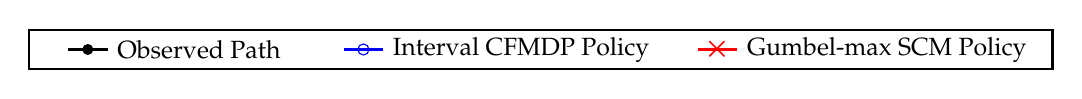
\begin{tikzpicture}[scale=1.0, every node/.style={scale=1.0}]
            \draw[thick, black] (-3, -0.25) rectangle (10, 0.25);
            %
            \draw[black, line width=1pt] (-2.5, 0.0) -- (-2,0.0);
            \fill[black] (-2.25,0.0) circle (2pt); %
            \node[right] at (-2,0.0) {\small Observed Path};
            
            %
            \draw[blue, line width=1pt] (1.0,0.0) -- (1.5,0.0);
            \node[draw=blue, circle, minimum size=4pt, inner sep=0pt] at (1.25,0.0) {}; %
            \node[right] at (1.5,0.0) {\small Interval CFMDP Policy};
            
            %
            \draw[red, line width=1pt] (5.5,0) -- (6,0);
            \node[red] at (5.75,0) {$\boldsymbol{\times}$}; %
            \node[right] at (6,0) {\small Gumbel-max SCM Policy};
        \end{tikzpicture}
    }\\
    %
    \subfigure[\footnotesize Lowest cumulative reward: Interval CFMDP ($312$), Gumbel-max SCM ($312$)]{%
        \resizebox{0.76\columnwidth}{!}{
             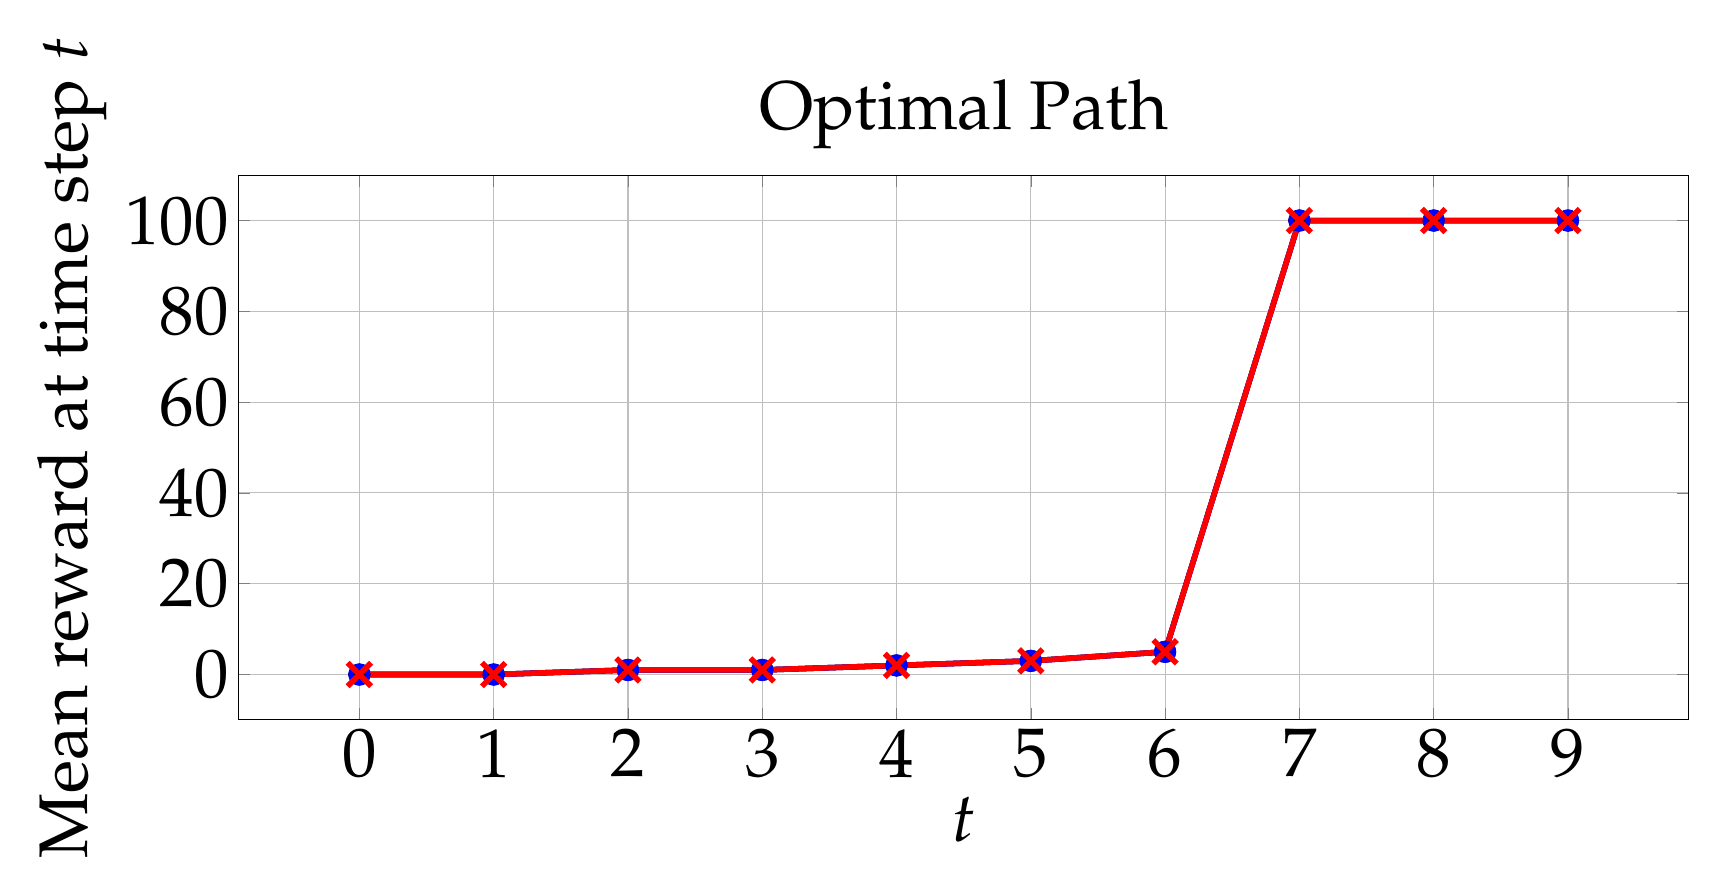
\begin{tikzpicture}
                \begin{axis}[
                    xlabel={$t$},
                    ylabel={Mean reward at time step $t$},
                    title={Optimal Path},
                    grid=both,
                    width=20cm, height=8.5cm,
                    every axis/.style={font=\Huge},
                    %
                ]
                \addplot[
                    color=black, %
                    mark=*, %
                    line width=2pt,
                    mark size=3pt,
                    error bars/.cd,
                    y dir=both, %
                    y explicit, %
                    error bar style={line width=1pt,solid},
                    error mark options={line width=1pt,mark size=4pt,rotate=90}
                ]
                coordinates {
                    (0, 0.0)  +- (0, 0.0)
                    (1, 0.0)  +- (0, 0.0) 
                    (2, 1.0)  +- (0, 0.0) 
                    (3, 1.0)  +- (0, 0.0)
                    (4, 2.0)  +- (0, 0.0)
                    (5, 3.0) +- (0, 0.0)
                    (6, 5.0) +- (0, 0.0)
                    (7, 100.0) +- (0, 0.0)
                    (8, 100.0) +- (0, 0.0)
                    (9, 100.0) +- (0, 0.0)
                };
                %
                \addplot[
                    color=blue, %
                    mark=o, %
                    line width=2pt,
                    mark size=3pt,
                    error bars/.cd,
                    y dir=both, %
                    y explicit, %
                    error bar style={line width=1pt,solid},
                    error mark options={line width=1pt,mark size=4pt,rotate=90}
                ]
                 coordinates {
                    (0, 0.0)  +- (0, 0.0)
                    (1, 0.0)  +- (0, 0.0) 
                    (2, 1.0)  +- (0, 0.0) 
                    (3, 1.0)  +- (0, 0.0)
                    (4, 2.0)  +- (0, 0.0)
                    (5, 3.0) +- (0, 0.0)
                    (6, 5.0) +- (0, 0.0)
                    (7, 100.0) +- (0, 0.0)
                    (8, 100.0) +- (0, 0.0)
                    (9, 100.0) +- (0, 0.0)
                };
                %
                \addplot[
                    color=red, %
                    mark=x, %
                    line width=2pt,
                    mark size=6pt,
                    error bars/.cd,
                    y dir=both, %
                    y explicit, %
                    error bar style={line width=1pt,solid},
                    error mark options={line width=1pt,mark size=4pt,rotate=90}
                ]
                coordinates {
                    (0, 0.0)  +- (0, 0.0)
                    (1, 0.0)  +- (0, 0.0) 
                    (2, 1.0)  +- (0, 0.0) 
                    (3, 1.0)  +- (0, 0.0)
                    (4, 2.0)  +- (0, 0.0)
                    (5, 3.0) +- (0, 0.0)
                    (6, 5.0) +- (0, 0.0)
                    (7, 100.0) +- (0, 0.0)
                    (8, 100.0) +- (0, 0.0)
                    (9, 100.0) +- (0, 0.0)
                };
                \end{axis}
            \end{tikzpicture}
         }
    }
    \hspace{1cm}
    \subfigure[\footnotesize Lowest cumulative reward: Interval CFMDP ($19$), Gumbel-max SCM ($-88$)]{%
         \resizebox{0.76\columnwidth}{!}{
            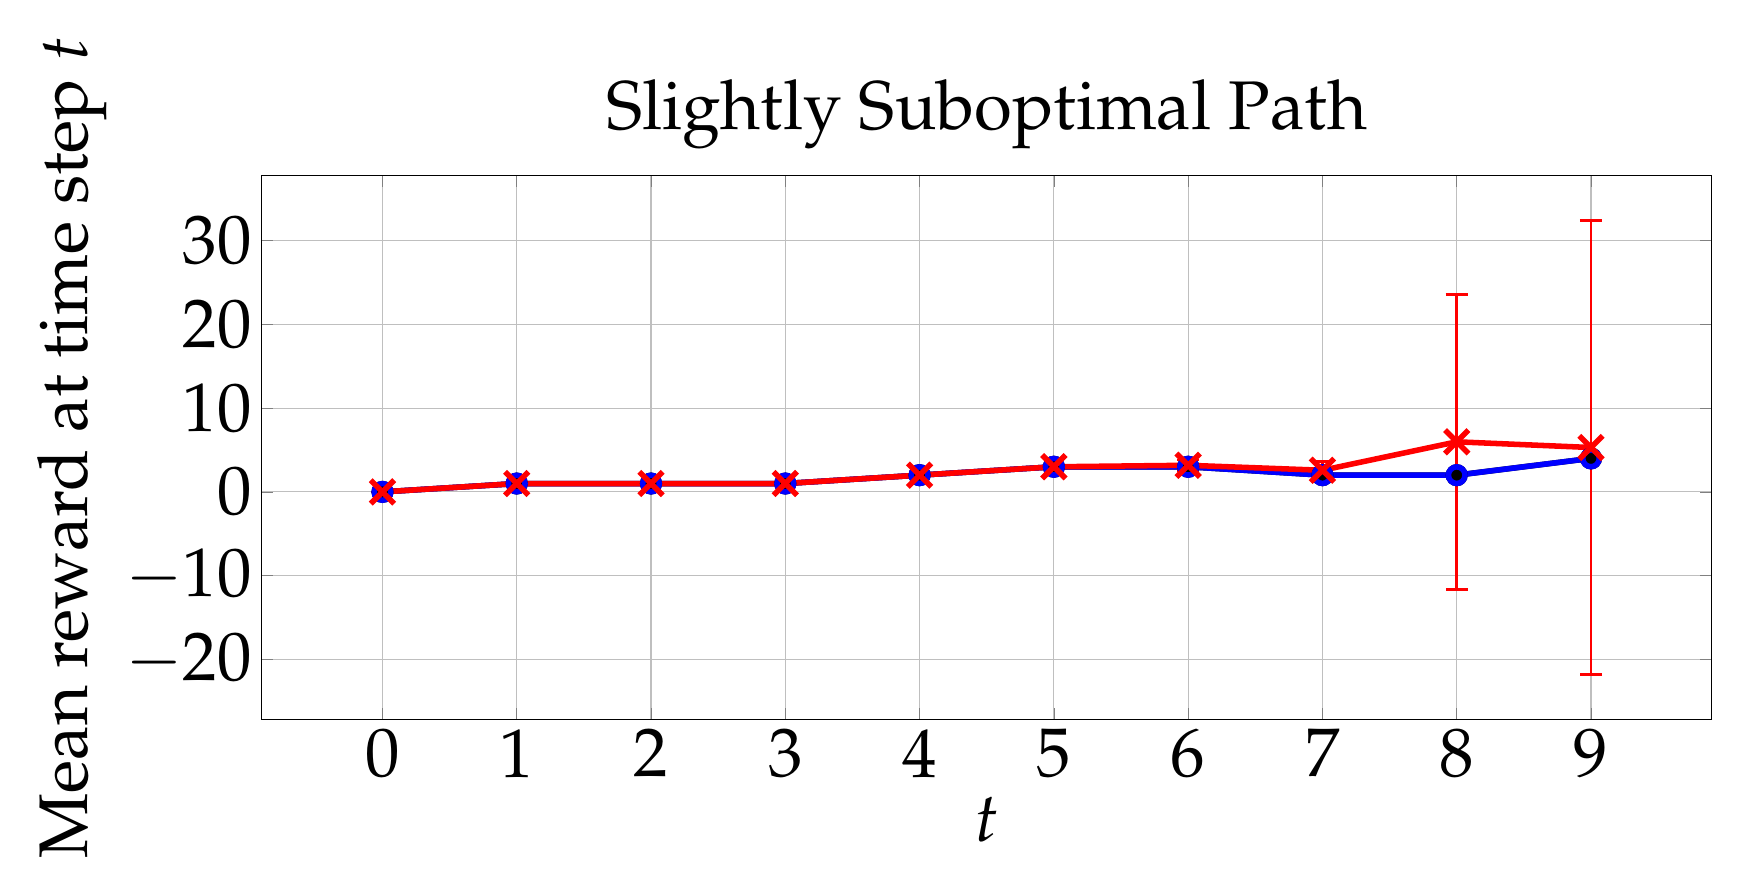
\begin{tikzpicture}
                \begin{axis}[
                    xlabel={$t$},
                    ylabel={Mean reward at time step $t$},
                    title={Slightly Suboptimal Path},
                    grid=both,
                    width=20cm, height=8.5cm,
                    every axis/.style={font=\Huge},
                    %
                ]
                \addplot[
                    color=black, %
                    mark=*, %
                    line width=2pt,
                    mark size=3pt,
                    error bars/.cd,
                    y dir=both, %
                    y explicit, %
                    error bar style={line width=1pt,solid},
                    error mark options={line width=1pt,mark size=4pt,rotate=90}
                ]
              coordinates {
                    (0, 0.0)  +- (0, 0.0)
                    (1, 1.0)  +- (0, 0.0) 
                    (2, 1.0)  +- (0, 0.0) 
                    (3, 1.0)  +- (0, 0.0)
                    (4, 2.0)  +- (0, 0.0)
                    (5, 3.0) +- (0, 0.0)
                    (6, 3.0) +- (0, 0.0)
                    (7, 2.0) +- (0, 0.0)
                    (8, 2.0) +- (0, 0.0)
                    (9, 4.0) +- (0, 0.0)
                };
                %
                \addplot[
                    color=blue, %
                    mark=o, %
                    line width=2pt,
                    mark size=3pt,
                    error bars/.cd,
                    y dir=both, %
                    y explicit, %
                    error bar style={line width=1pt,solid},
                    error mark options={line width=1pt,mark size=4pt,rotate=90}
                ]
              coordinates {
                    (0, 0.0)  +- (0, 0.0)
                    (1, 1.0)  +- (0, 0.0) 
                    (2, 1.0)  +- (0, 0.0) 
                    (3, 1.0)  +- (0, 0.0)
                    (4, 2.0)  +- (0, 0.0)
                    (5, 3.0) +- (0, 0.0)
                    (6, 3.0) +- (0, 0.0)
                    (7, 2.0) +- (0, 0.0)
                    (8, 2.0) +- (0, 0.0)
                    (9, 4.0) +- (0, 0.0)
                };
                %
                \addplot[
                    color=red, %
                    mark=x, %
                    line width=2pt,
                    mark size=6pt,
                    error bars/.cd,
                    y dir=both, %
                    y explicit, %
                    error bar style={line width=1pt,solid},
                    error mark options={line width=1pt,mark size=4pt,rotate=90}
                ]
                coordinates {
                    (0, 0.0)  +- (0, 0.0)
                    (1, 1.0)  +- (0, 0.0) 
                    (2, 1.0)  +- (0, 0.0) 
                    (3, 1.0)  +- (0, 0.0)
                    (4, 2.0)  += (0, 0.0)
                    (5, 3.0)  += (0, 0.0)
                    (6, 3.17847) += (0, 0.62606746) -= (0, 0.62606746)
                    (7, 2.5832885) += (0, 1.04598233) -= (0, 1.04598233)
                    (8, 5.978909) += (0, 17.60137623) -= (0, 17.60137623)
                    (9, 5.297059) += (0, 27.09227512) -= (0, 27.09227512)
                };
                \end{axis}
            \end{tikzpicture}
         }
    }\\[-1.5pt]
    \subfigure[\footnotesize Lowest cumulative reward: Interval CFMDP ($14$), Gumbel-max SCM ($-598$)]{%
         \resizebox{0.76\columnwidth}{!}{
             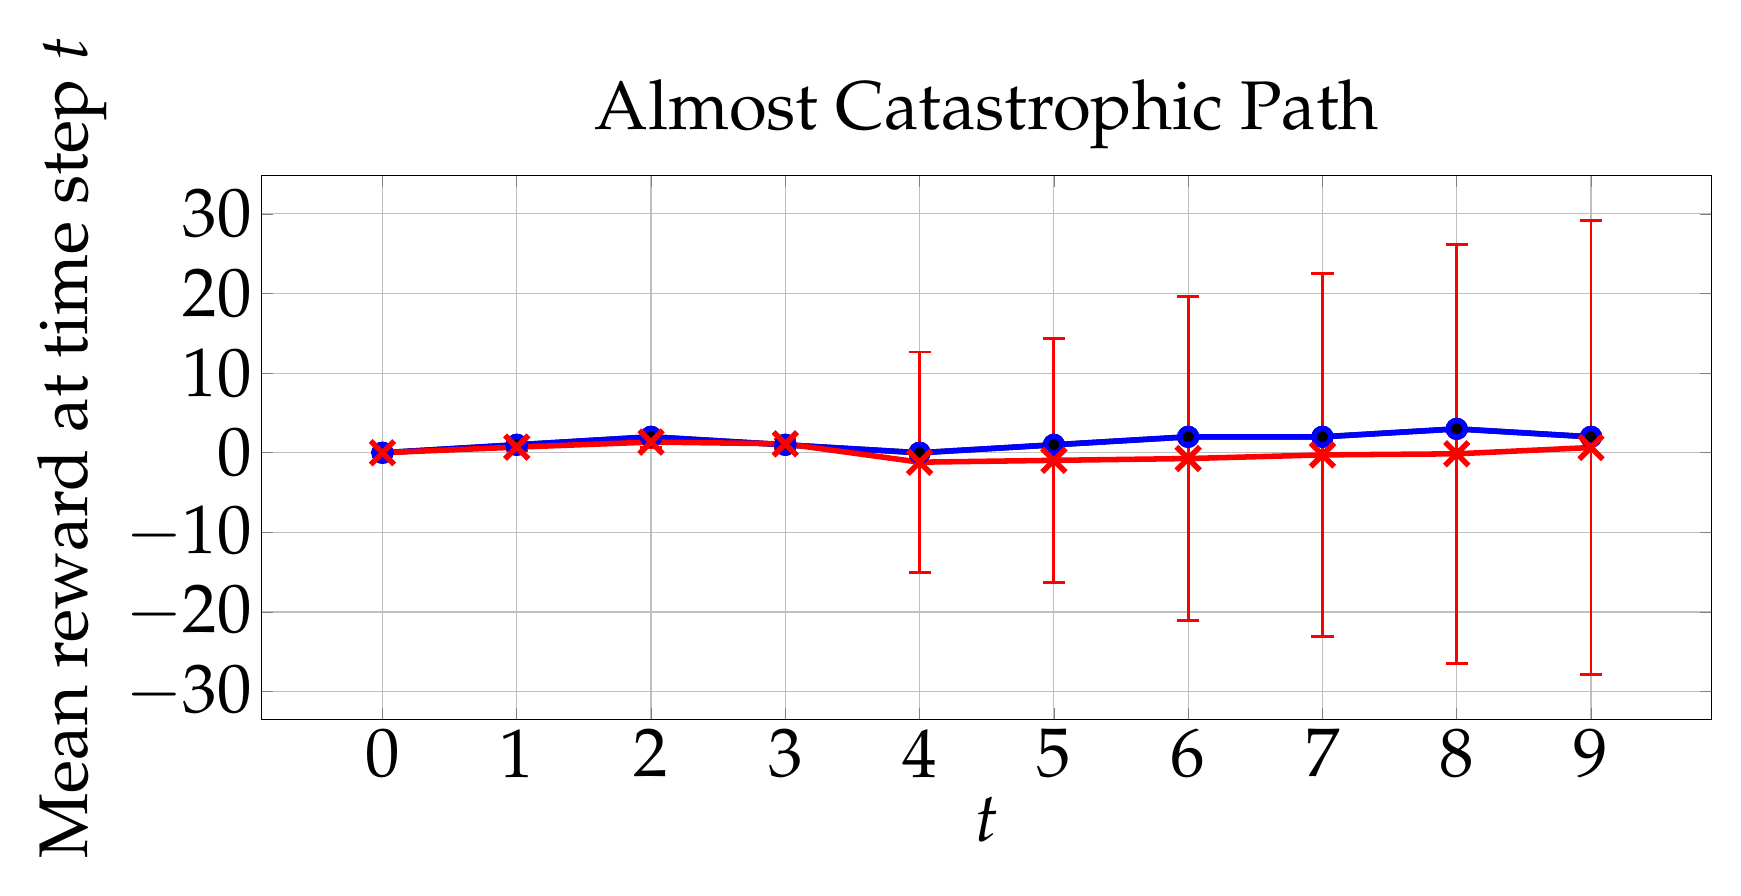
\begin{tikzpicture}
                \begin{axis}[
                    xlabel={$t$},
                    ylabel={Mean reward at time step $t$},
                    title={Almost Catastrophic Path},
                    grid=both,
                    width=20cm, height=8.5cm,
                    every axis/.style={font=\Huge},
                    %
                ]
                \addplot[
                    color=black, %
                    mark=*, %
                    line width=2pt,
                    mark size=3pt,
                    error bars/.cd,
                    y dir=both, %
                    y explicit, %
                    error bar style={line width=1pt,solid},
                    error mark options={line width=1pt,mark size=4pt,rotate=90}
                ]
                coordinates {
                    (0, 0.0)  +- (0, 0.0)
                    (1, 1.0)  +- (0, 0.0) 
                    (2, 2.0)  +- (0, 0.0) 
                    (3, 1.0)  +- (0, 0.0)
                    (4, 0.0)  +- (0, 0.0)
                    (5, 1.0) +- (0, 0.0)
                    (6, 2.0) +- (0, 0.0)
                    (7, 2.0) +- (0, 0.0)
                    (8, 3.0) +- (0, 0.0)
                    (9, 2.0) +- (0, 0.0)
                };
                %
                \addplot[
                    color=blue, %
                    mark=o, %
                    line width=2pt,
                    mark size=3pt,
                    error bars/.cd,
                    y dir=both, %
                    y explicit, %
                    error bar style={line width=1pt,solid},
                    error mark options={line width=1pt,mark size=4pt,rotate=90}
                ]
                coordinates {
                    (0, 0.0)  +- (0, 0.0)
                    (1, 1.0)  +- (0, 0.0) 
                    (2, 2.0)  +- (0, 0.0) 
                    (3, 1.0)  +- (0, 0.0)
                    (4, 0.0)  +- (0, 0.0)
                    (5, 1.0) +- (0, 0.0)
                    (6, 2.0) +- (0, 0.0)
                    (7, 2.0) +- (0, 0.0)
                    (8, 3.0) +- (0, 0.0)
                    (9, 2.0) +- (0, 0.0)
                };
                %
                \addplot[
                    color=red, %
                    mark=x, %
                    line width=2pt,
                    mark size=6pt,
                    error bars/.cd,
                    y dir=both, %
                    y explicit, %
                    error bar style={line width=1pt,solid},
                    error mark options={line width=1pt,mark size=4pt,rotate=90}
                ]
                coordinates {
                    (0, 0.0)  +- (0, 0.0)
                    (1, 0.7065655)  +- (0, 0.4553358) 
                    (2, 1.341673)  +- (0, 0.67091621) 
                    (3, 1.122926)  +- (0, 0.61281824)
                    (4, -1.1821935)  +- (0, 13.82444042)
                    (5, -0.952399)  +- (0, 15.35195457)
                    (6, -0.72672) +- (0, 20.33508414)
                    (7, -0.268983) +- (0, 22.77861454)
                    (8, -0.1310835) +- (0, 26.31013314)
                    (9, 0.65806) +- (0, 28.50670214)
                };
                %
            %
            %
            %
            %
            %
            %
            %
            %
            %
            %
            %
            %
            %
            %
            %
            %
            %
            %
                \end{axis}
            \end{tikzpicture}
         }
    }
    \hspace{1cm}
    \subfigure[\footnotesize Lowest cumulative reward: Interval CFMDP ($-698$), Gumbel-max SCM ($-698$)]{%
         \resizebox{0.76\columnwidth}{!}{
            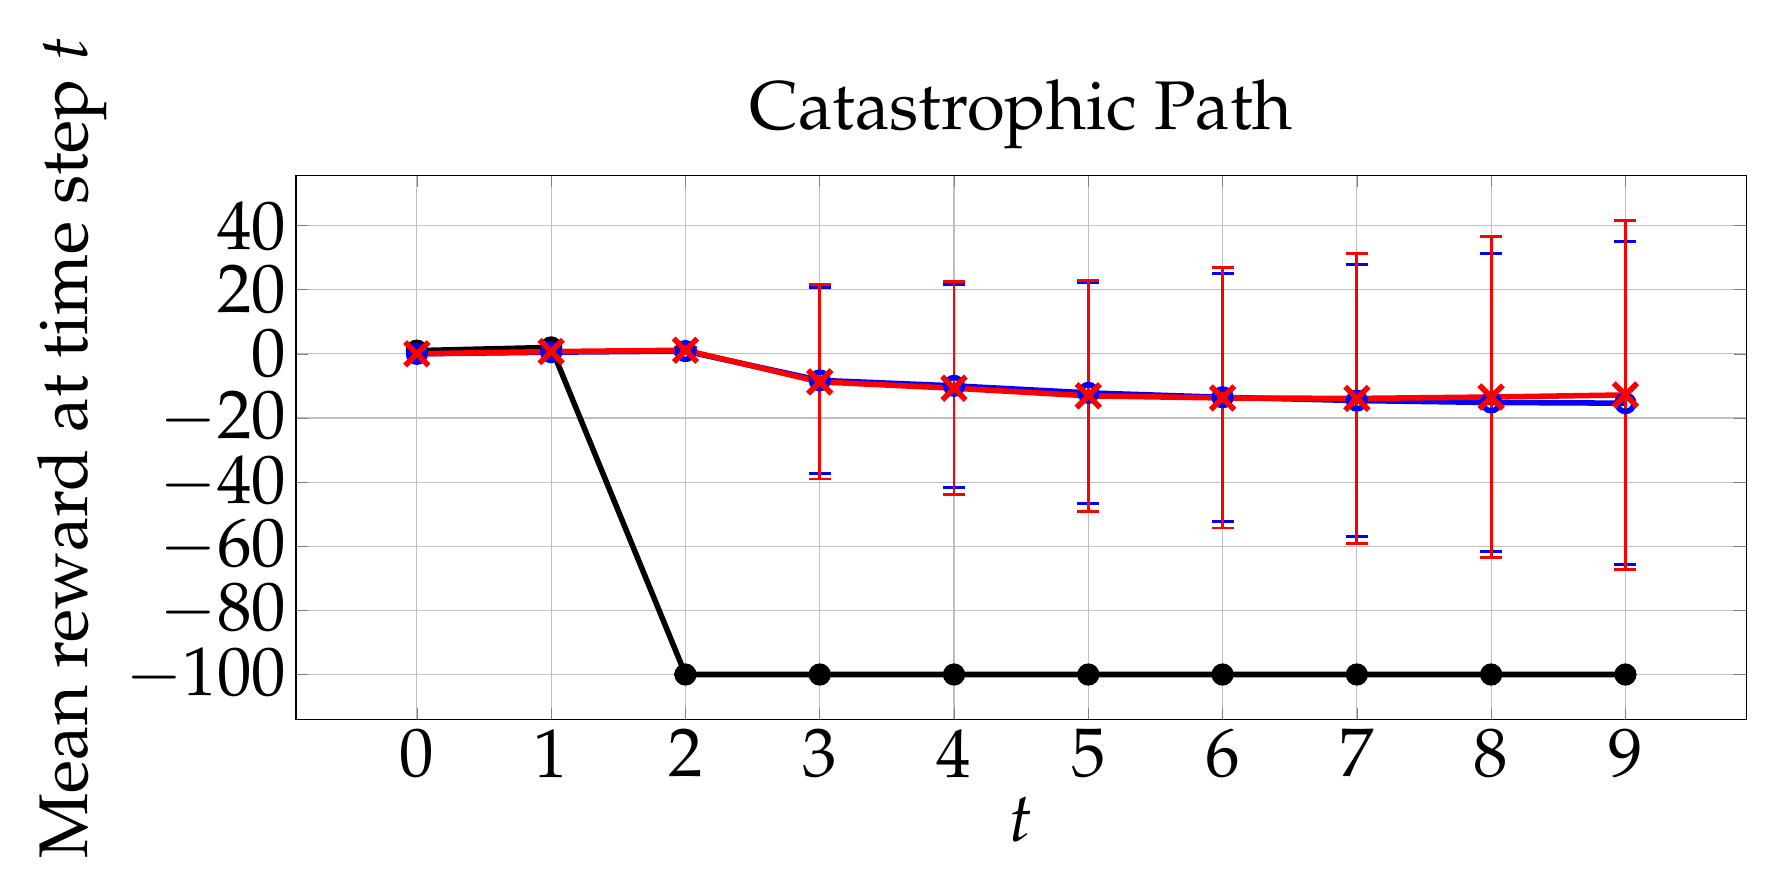
\begin{tikzpicture}
                \begin{axis}[
                    xlabel={$t$},
                    ylabel={Mean reward at time step $t$},
                    title={Catastrophic Path},
                    grid=both,
                    width=20cm, height=8.5cm,
                    every axis/.style={font=\Huge},
                    %
                ]
                \addplot[
                    color=black, %
                    mark=*, %
                    line width=2pt,
                    mark size=3pt,
                    error bars/.cd,
                    y dir=both, %
                    y explicit, %
                    error bar style={line width=1pt,solid},
                    error mark options={line width=1pt,mark size=4pt,rotate=90}
                ]
                coordinates {
                    (0, 1.0)  +- (0, 0.0)
                    (1, 2.0)  +- (0, 0.0) 
                    (2, -100.0)  +- (0, 0.0) 
                    (3, -100.0)  +- (0, 0.0)
                    (4, -100.0)  +- (0, 0.0)
                    (5, -100.0) +- (0, 0.0)
                    (6, -100.0) +- (0, 0.0)
                    (7, -100.0) +- (0, 0.0)
                    (8, -100.0) +- (0, 0.0)
                    (9, -100.0) +- (0, 0.0)
                };
                %
                \addplot[
                    color=blue, %
                    mark=o, %
                    line width=2pt,
                    mark size=3pt,
                    error bars/.cd,
                    y dir=both, %
                    y explicit, %
                    error bar style={line width=1pt,solid},
                    error mark options={line width=1pt,mark size=4pt,rotate=90}
                ]
                coordinates {
                    (0, 0.0)  +- (0, 0.0)
                    (1, 0.504814)  +- (0, 0.49997682) 
                    (2, 0.8439835)  +- (0, 0.76831917) 
                    (3, -8.2709165)  +- (0, 28.93656754)
                    (4, -9.981082)  +- (0, 31.66825363)
                    (5, -12.1776325) +- (0, 34.53463233)
                    (6, -13.556076) +- (0, 38.62845372)
                    (7, -14.574418) +- (0, 42.49603359)
                    (8, -15.1757075) +- (0, 46.41913968)
                    (9, -15.3900395) +- (0, 50.33563368)
                };
                %
                \addplot[
                    color=red, %
                    mark=x, %
                    line width=2pt,
                    mark size=6pt,
                    error bars/.cd,
                    y dir=both, %
                    y explicit, %
                    error bar style={line width=1pt,solid},
                    error mark options={line width=1pt,mark size=4pt,rotate=90}
                ]
                coordinates {
                    (0, 0.0)  +- (0, 0.0)
                    (1, 0.701873)  +- (0, 0.45743556) 
                    (2, 1.1227805)  +- (0, 0.73433129) 
                    (3, -8.7503255)  +- (0, 30.30257976)
                    (4, -10.722092)  +- (0, 33.17618589)
                    (5, -13.10721)  +- (0, 36.0648089)
                    (6, -13.7631645) +- (0, 40.56553451)
                    (7, -13.909043) +- (0, 45.23829402)
                    (8, -13.472517) +- (0, 49.96270296)
                    (9, -12.8278835) +- (0, 54.38618735)
                };
                %
            %
            %
            %
            %
            %
            %
            %
            %
            %
            %
            %
            %
            %
            %
            %
            %
            %
            %
                \end{axis}
            \end{tikzpicture}
         }
    }
    \caption{Average instant reward of CF paths induced by policies on GridWorld $p=0.4$.}
    \label{fig: reward p=0.4}
\end{figure*}

\subsection{Experimental Setup}
To compare policy performance, we measure the average rewards of counterfactual paths induced by our policy and the Gumbel-max policy by uniformly sampling $200$ counterfactual MDPs from the ICFMDP and generating $10,000$ counterfactual paths over each sampled CFMDP. \jl{Since the interval CFMDP depends on the observed path, we select $4$  paths of varying optimality to evaluate how the observed path impacts the performance of both policies: an optimal path, a slightly suboptimal path that could reach the optimal reward with a few changes, a catastrophic path that enters a catastrophic, terminal state with low reward, and an almost catastrophic path that was close to entering a catastrophic state.} When measuring the average probability bound widths and execution time needed to generate the ICFMDPs, we averaged over $20$ randomly generated observed paths
\footnote{Further training details are provided in Appendix \ref{app: training details}, and the code is provided at \href{https://github.com/ddv-lab/robust-cf-inference-in-MDPs}{https://github.com/ddv-lab/robust-cf-inference-in-MDPs}
%
%
.}.

\subsection{GridWorld}
\jl{The GridWorld MDP is a $4 \times 4$ grid where an agent must navigate from the top-left corner to the goal state in the bottom-right corner, avoiding a dangerous terminal state in the centre. At each time step, the agent can move up, down, left, or right, but there is a small probability (controlled by hyper-parameter $p$) of moving in an unintended direction. As the agent nears the goal, the reward for each state increases, culminating in a reward of $+100$ for reaching the goal. Entering the dangerous state results in a penalty of $-100$. We use two versions of GridWorld: a less stochastic version with $p=0.9$ (i.e., $90$\% chance of moving in the chosen direction) and a more stochastic version with $p=0.4$.}

\paragraph{GridWorld ($p=0.9$)}
When $p=0.9$, the counterfactual probability bounds are typically narrow (see Table \ref{tab:nonzero_probs} for average measurements). Consequently, as shown in Figure \ref{fig: reward p=0.9}, both policies are nearly identical and perform similarly well across the optimal, slightly suboptimal, and catastrophic paths.
%
However, for the almost catastrophic path, the interval CFMDP path is more conservative and follows the observed path more closely (as this is where the probability bounds are narrowest), which typically requires one additional step to reach the goal state than the Gumbel-max SCM policy.
%

\paragraph{GridWorld ($p=0.4$)}
\jl{When $p=0.4$, the GridWorld environment becomes more uncertain, increasing the risk of entering the dangerous state even if correct actions are chosen. Thus, as shown in Figure \ref{fig: reward p=0.4}, the interval CFMDP policy adopts a more conservative approach, avoiding deviation from the observed policy if it cannot guarantee higher counterfactual rewards (see the slightly suboptimal and almost catastrophic paths), whereas the Gumbel-max SCM is inconsistent: it can yield higher rewards, but also much lower rewards, reflected in the wide error bars.} For the catastrophic path, both policies must deviate from the observed path to achieve a higher reward and, in this case, perform similarly.
%
%
%
%
\subsection{Sepsis}
The Sepsis MDP \citep{oberst2019counterfactual} simulates trajectories of Sepsis patients. Each state consists of four vital signs (heart rate, blood pressure, oxygen concentration, and glucose levels), categorised as low, normal, or high.
and three treatments that can be toggled on/off at each time step (8 actions in total). Unlike \citet{oberst2019counterfactual}, we scale rewards based on the number of out-of-range vital signs, between $-1000$ (patient dies) and $1000$ (patient discharged). \jl{Like the GridWorld $p=0.4$ experiment, the Sepsis MDP is highly uncertain, as many states are equally likely to lead to optimal and poor outcomes. Thus, as shown in Figure \ref{fig: reward sepsis}, both policies follow the observed optimal and almost catastrophic paths to guarantee rewards are no worse than the observation.} However, improving the catastrophic path requires deviating from the observation. Here, the Gumbel-max SCM policy, on average, performs better than the interval CFMDP policy. But, since both policies have lower bounds clipped at $-1000$, neither policy reliably improves over the observation. In contrast, for the slightly suboptimal path, the interval CFMDP policy performs significantly better, shown by its higher lower bounds. 
Moreover, in these two cases, the worst-case counterfactual path generated by the interval CFMDP policy is better than that of the Gumbel-max SCM policy,
indicating its greater robustness.
%
\begin{figure*}
    \centering
     \resizebox{0.6\textwidth}{!}{
        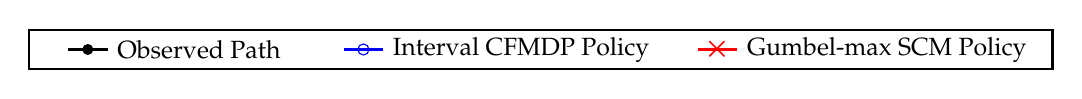
\begin{tikzpicture}[scale=1.0, every node/.style={scale=1.0}]
            \draw[thick, black] (-3, -0.25) rectangle (10, 0.25);
            %
            \draw[black, line width=1pt] (-2.5, 0.0) -- (-2,0.0);
            \fill[black] (-2.25,0.0) circle (2pt); %
            \node[right] at (-2,0.0) {\small Observed Path};
            
            %
            \draw[blue, line width=1pt] (1.0,0.0) -- (1.5,0.0);
            \node[draw=blue, circle, minimum size=4pt, inner sep=0pt] at (1.25,0.0) {}; %
            \node[right] at (1.5,0.0) {\small Interval CFMDP Policy};
            
            %
            \draw[red, line width=1pt] (5.5,0) -- (6,0);
            \node[red] at (5.75,0) {$\boldsymbol{\times}$}; %
            \node[right] at (6,0) {\small Gumbel-max SCM Policy};
        \end{tikzpicture}
    }\\
    \subfigure[\footnotesize Lowest cumulative reward: Interval CFMDP ($8000$), Gumbel-max SCM ($8000$)]{%
         \resizebox{0.76\columnwidth}{!}{
             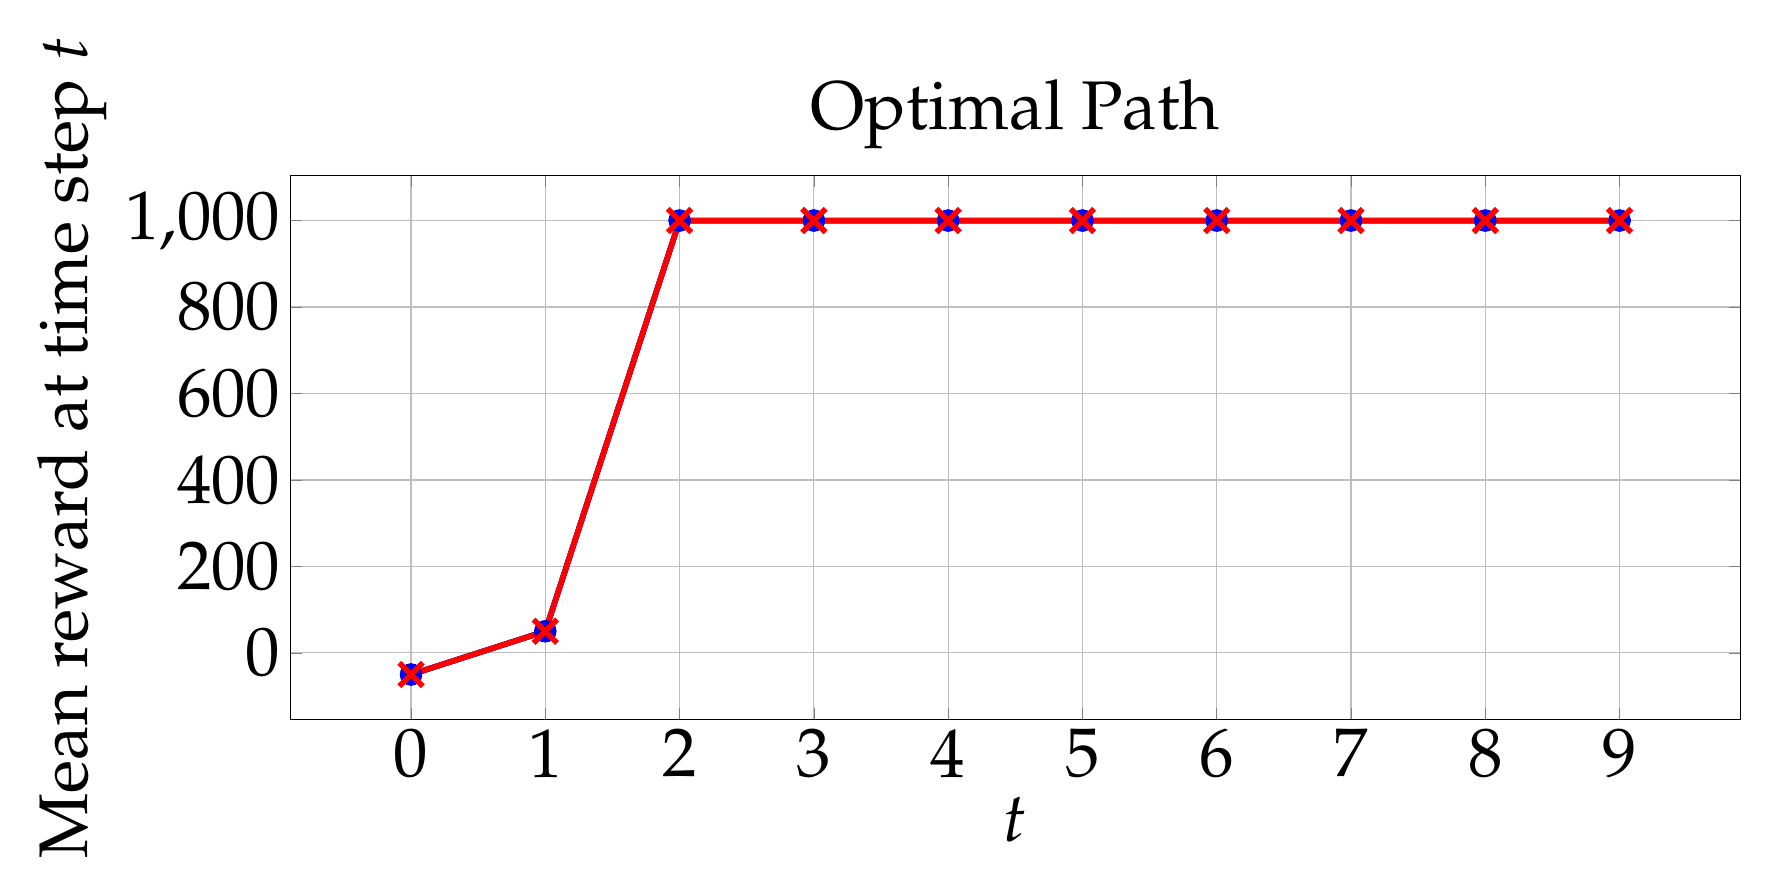
\begin{tikzpicture}
                \begin{axis}[
                    xlabel={$t$},
                    ylabel={Mean reward at time step $t$},
                    title={Optimal Path},
                    grid=both,
                    width=20cm, height=8.5cm,
                    every axis/.style={font=\Huge},
                    %
                ]
                \addplot[
                    color=black, %
                    mark=*, %
                    line width=2pt,
                    mark size=3pt,
                ]
                coordinates {
                    (0, -50.0)
                    (1, 50.0)
                    (2, 1000.0)
                    (3, 1000.0)
                    (4, 1000.0)
                    (5, 1000.0)
                    (6, 1000.0)
                    (7, 1000.0)
                    (8, 1000.0)
                    (9, 1000.0)
                };
                %
                \addplot[
                    color=blue, %
                    mark=o, %
                    line width=2pt,
                    mark size=3pt,
                    error bars/.cd,
                    y dir=both, %
                    y explicit, %
                    error bar style={line width=1pt,solid},
                    error mark options={line width=1pt,mark size=4pt,rotate=90}
                ]
                coordinates {
                    (0, -50.0)  +- (0, 0.0)
                    (1, 50.0)  +- (0, 0.0) 
                    (2, 1000.0)  +- (0, 0.0) 
                    (3, 1000.0)  +- (0, 0.0)
                    (4, 1000.0)  +- (0, 0.0)
                    (5, 1000.0) +- (0, 0.0)
                    (6, 1000.0) +- (0, 0.0)
                    (7, 1000.0) +- (0, 0.0)
                    (8, 1000.0) +- (0, 0.0)
                    (9, 1000.0) +- (0, 0.0)
                };
                %
                \addplot[
                    color=red, %
                    mark=x, %
                    line width=2pt,
                    mark size=6pt,
                    error bars/.cd,
                    y dir=both, %
                    y explicit, %
                    error bar style={line width=1pt,solid},
                    error mark options={line width=1pt,mark size=4pt,rotate=90}
                ]
                coordinates {
                    (0, -50.0)  +- (0, 0.0)
                    (1, 50.0)  +- (0, 0.0) 
                    (2, 1000.0)  +- (0, 0.0) 
                    (3, 1000.0)  +- (0, 0.0)
                    (4, 1000.0)  +- (0, 0.0)
                    (5, 1000.0) +- (0, 0.0)
                    (6, 1000.0) +- (0, 0.0)
                    (7, 1000.0) +- (0, 0.0)
                    (8, 1000.0) +- (0, 0.0)
                    (9, 1000.0) +- (0, 0.0)
                };
                %
                \end{axis}
            \end{tikzpicture}
         }
    }
    \hspace{1cm}
    \subfigure[\footnotesize Lowest cumulative reward: Interval CFMDP ($-5980$), Gumbel-max SCM ($-8000$)]{%
         \resizebox{0.76\columnwidth}{!}{
            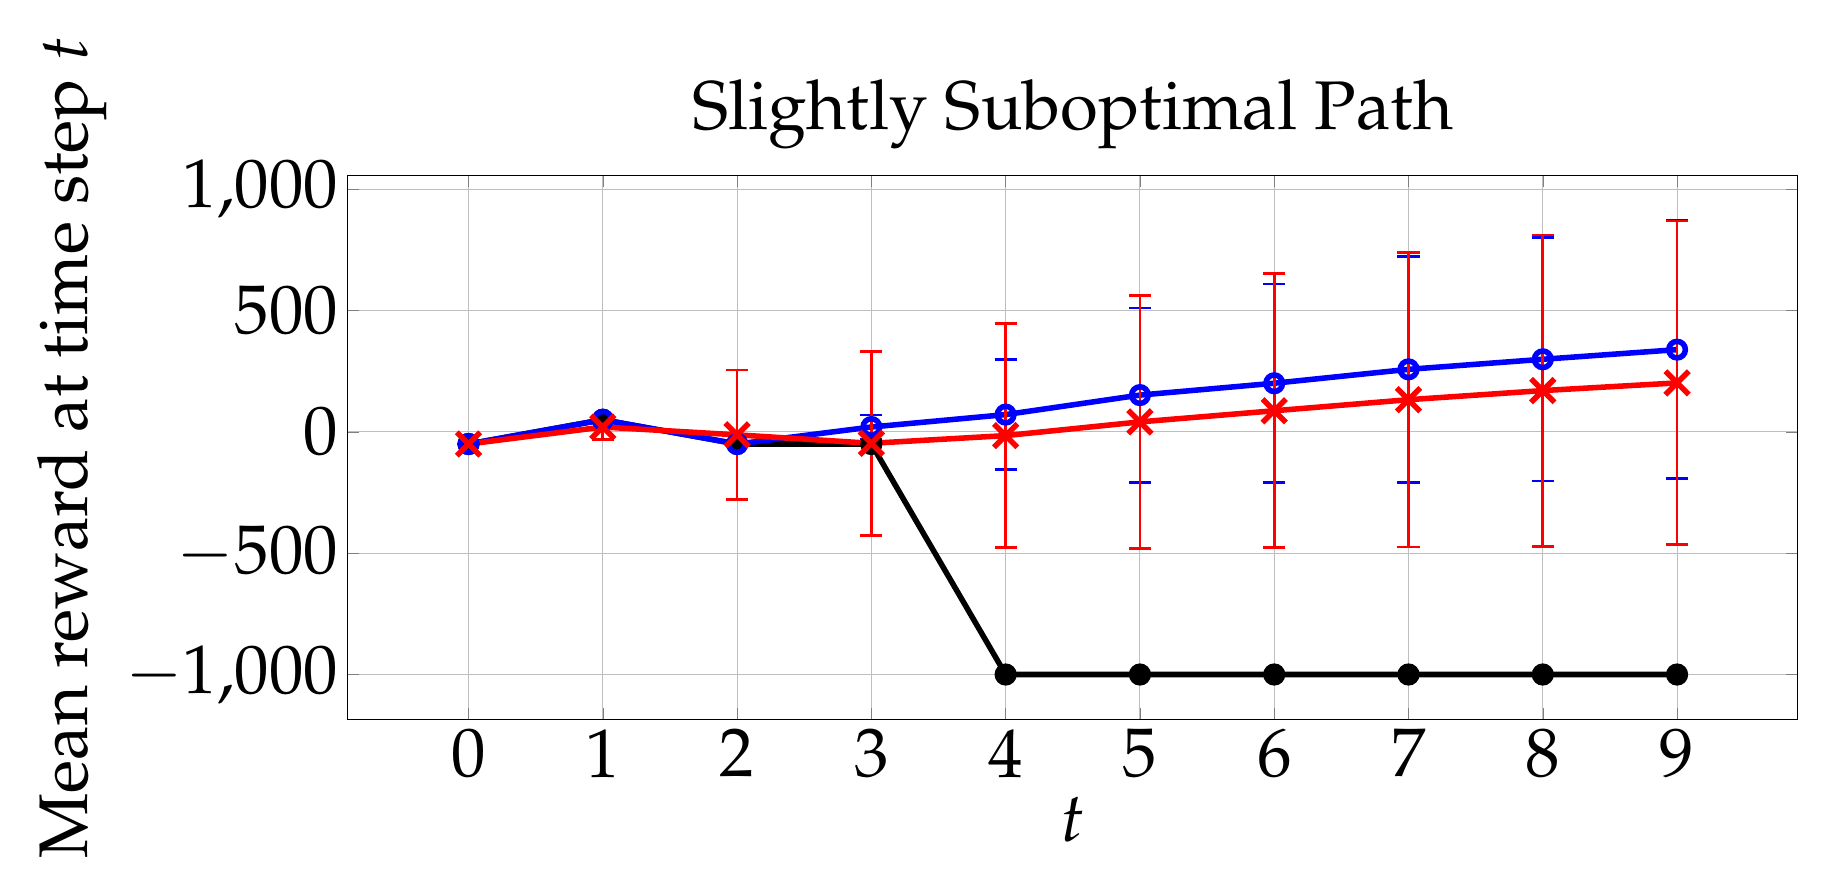
\begin{tikzpicture}
                \begin{axis}[
                    xlabel={$t$},
                    ylabel={Mean reward at time step $t$},
                    title={Slightly Suboptimal Path},
                    grid=both,
                    width=20cm, height=8.5cm,
                    every axis/.style={font=\Huge},
                    %
                ]
               \addplot[
                    color=black, %
                    mark=*, %
                    line width=2pt,
                    mark size=3pt,
                ]
                coordinates {
                    (0, -50.0)
                    (1, 50.0)
                    (2, -50.0)
                    (3, -50.0)
                    (4, -1000.0)
                    (5, -1000.0)
                    (6, -1000.0)
                    (7, -1000.0)
                    (8, -1000.0)
                    (9, -1000.0)
                };
                %
                \addplot[
                    color=blue, %
                    mark=o, %
                    line width=2pt,
                    mark size=3pt,
                    error bars/.cd,
                    y dir=both, %
                    y explicit, %
                    error bar style={line width=1pt,solid},
                    error mark options={line width=1pt,mark size=4pt,rotate=90}
                ]
                coordinates {
                    (0, -50.0)  +- (0, 0.0)
                    (1, 50.0)  +- (0, 0.0) 
                    (2, -50.0)  +- (0, 0.0) 
                    (3, 20.0631)  +- (0, 49.97539413)
                    (4, 71.206585)  +- (0, 226.02033693)
                    (5, 151.60797) +- (0, 359.23292559)
                    (6, 200.40593) +- (0, 408.86185176)
                    (7, 257.77948) +- (0, 466.10372804)
                    (8, 299.237465) +- (0, 501.82579506)
                    (9, 338.9129) +- (0, 532.06124996)
                };
                %
                \addplot[
                    color=red, %
                    mark=x, %
                    line width=2pt,
                    mark size=6pt,
                    error bars/.cd,
                    y dir=both, %
                    y explicit, %
                    error bar style={line width=1pt,solid},
                    error mark options={line width=1pt,mark size=4pt,rotate=90}
                ]
                coordinates {
                    (0, -50.0)  +- (0, 0.0)
                    (1, 20.00736)  +- (0, 49.99786741) 
                    (2, -12.282865)  +- (0, 267.598755) 
                    (3, -47.125995)  +- (0, 378.41755832)
                    (4, -15.381965)  +- (0, 461.77616558)
                    (5, 41.15459) +- (0, 521.53189262)
                    (6, 87.01595) +- (0, 564.22243126 )
                    (7, 132.62376) +- (0, 607.31338037)
                    (8, 170.168145) +- (0, 641.48013693)
                    (9, 201.813135) +- (0, 667.29441777)
                };
                %
                %
                %
                %
                %
                %
                %
                %
                %
                %
                %
                %
                %
                %
                %
                %
                %
                %
                %
                \end{axis}
            \end{tikzpicture}
         }
    }\\[-1.5pt]
    \subfigure[\footnotesize Lowest cumulative reward: Interval CFMDP ($100$), Gumbel-max SCM ($100$)]{%
         \resizebox{0.76\columnwidth}{!}{
             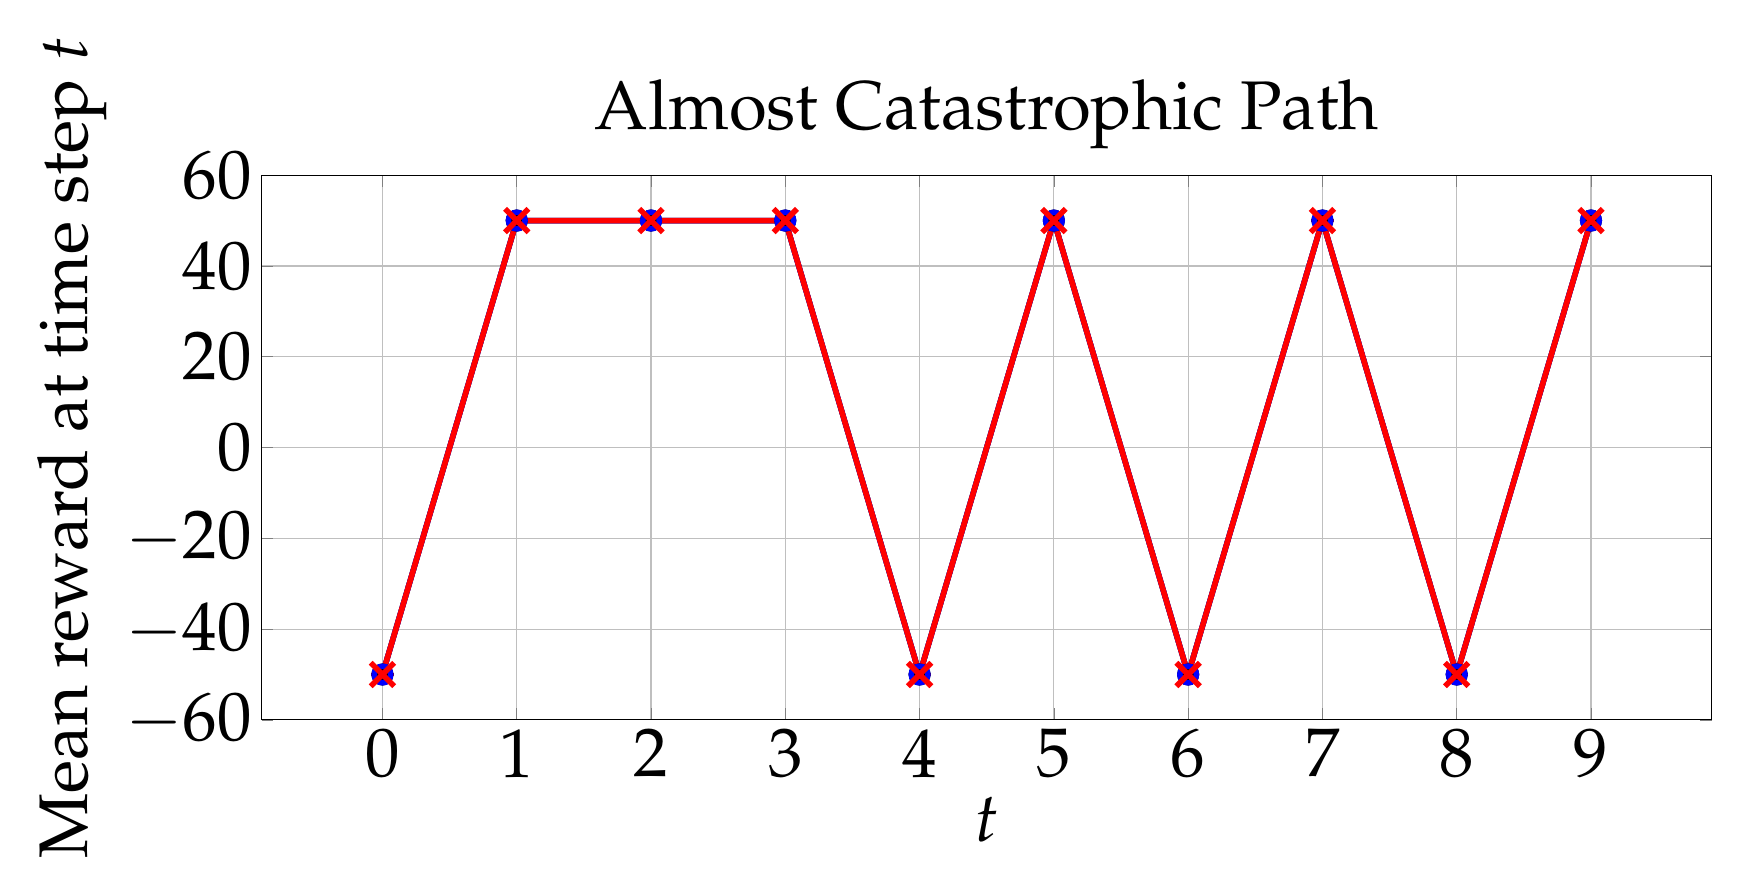
\begin{tikzpicture}
                \begin{axis}[
                    xlabel={$t$},
                    ylabel={Mean reward at time step $t$},
                    title={Almost Catastrophic Path},
                    grid=both,
                    every axis/.style={font=\Huge},
                    width=20cm, height=8.5cm,
                    %
                ]
               \addplot[
                    color=black, %
                    mark=*, %
                    line width=2pt,
                    mark size=3pt,
                ]
                coordinates {
                    (0, -50.0)
                    (1, 50.0)
                    (2, 50.0)
                    (3, 50.0)
                    (4, -50.0)
                    (5, 50.0)
                    (6, -50.0)
                    (7, 50.0)
                    (8, -50.0)
                    (9, 50.0)
                };
                %
                %
                \addplot[
                    color=blue, %
                    mark=o, %
                    line width=2pt,
                    mark size=3pt,
                    error bars/.cd,
                    y dir=both, %
                    y explicit, %
                    error bar style={line width=1pt,solid},
                    error mark options={line width=1pt,mark size=4pt,rotate=90}
                ]
                coordinates {
                    (0, -50.0)  +- (0, 0.0)
                    (1, 50.0)  +- (0, 0.0) 
                    (2, 50.0)  +- (0, 0.0) 
                    (3, 50.0)  +- (0, 0.0)
                    (4, -50.0)  +- (0, 0.0)
                    (5, 50.0) +- (0, 0.0)
                    (6, -50.0) +- (0, 0.0)
                    (7, 50.0) +- (0, 0.0)
                    (8, -50.0) +- (0, 0.0)
                    (9, 50.0) +- (0, 0.0)
                };
                %
                \addplot[
                    color=red, %
                    mark=x, %
                    line width=2pt,
                    mark size=6pt,
                    error bars/.cd,
                    y dir=both, %
                    y explicit, %
                    error bar style={line width=1pt,solid},
                    error mark options={line width=1pt,mark size=4pt,rotate=90}
                ]
                coordinates {
                    (0, -50.0)  +- (0, 0.0)
                    (1, 50.0)  +- (0, 0.0) 
                    (2, 50.0)  +- (0, 0.0) 
                    (3, 50.0)  +- (0, 0.0)
                    (4, -50.0)  +- (0, 0.0)
                    (5, 50.0) +- (0, 0.0)
                    (6, -50.0) +- (0, 0.0)
                    (7, 50.0) +- (0, 0.0)
                    (8, -50.0) +- (0, 0.0)
                    (9, 50.0) +- (0, 0.0)
                };
                %
                %
                %
                %
                %
                %
                %
                %
                %
                %
                %
                %
                %
                %
                %
                %
                %
                %
                %
                \end{axis}
            \end{tikzpicture}
         }
    }
    \hspace{1cm}
    \subfigure[\footnotesize Lowest cumulative reward: Interval CFMDP ($-7150$), Gumbel-max SCM ($-9050$)]{%
         \resizebox{0.76\columnwidth}{!}{
            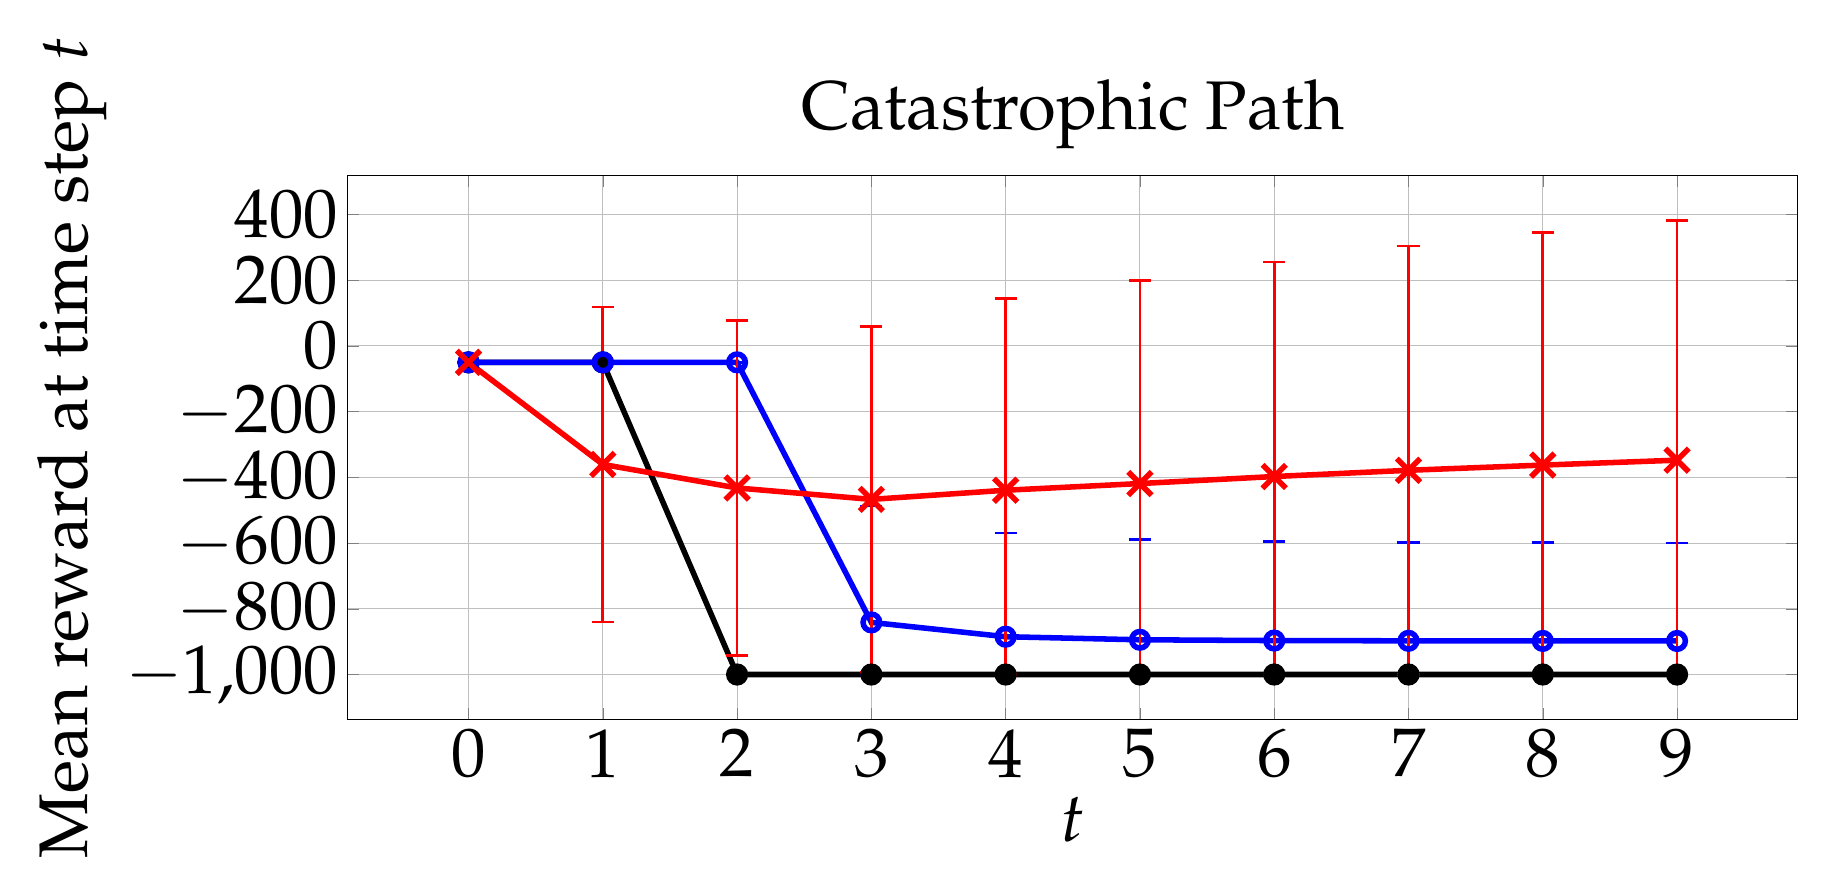
\begin{tikzpicture}
                \begin{axis}[
                    xlabel={$t$},
                    ylabel={Mean reward at time step $t$},
                    title={Catastrophic Path},
                    grid=both,
                    width=20cm, height=8.5cm,
                    every axis/.style={font=\Huge},
                    %
                ]
               \addplot[
                    color=black, %
                    mark=*, %
                    line width=2pt,
                    mark size=3pt,
                ]
                coordinates {
                    (0, -50.0)
                    (1, -50.0)
                    (2, -1000.0)
                    (3, -1000.0)
                    (4, -1000.0)
                    (5, -1000.0)
                    (6, -1000.0)
                    (7, -1000.0)
                    (8, -1000.0)
                    (9, -1000.0)
                };
                %
                %
                \addplot[
                    color=blue, %
                    mark=o, %
                    line width=2pt,
                    mark size=3pt,
                    error bars/.cd,
                    y dir=both, %
                    y explicit, %
                    error bar style={line width=1pt,solid},
                    error mark options={line width=1pt,mark size=4pt,rotate=90}
                ]
                coordinates {
                    (0, -50.0)  +- (0, 0.0)
                    (1, -50.0)  +- (0, 0.0) 
                    (2, -50.0)  +- (0, 0.0) 
                    (3, -841.440725)  += (0, 354.24605512) -= (0, 158.559275)
                    (4, -884.98225)  += (0, 315.37519669) -= (0, 115.01775)
                    (5, -894.330425) += (0, 304.88572805) -= (0, 105.669575)
                    (6, -896.696175) += (0, 301.19954514) -= (0, 103.303825)
                    (7, -897.4635) += (0, 299.61791279) -= (0, 102.5365)
                    (8, -897.77595) += (0, 298.80392585) -= (0, 102.22405)
                    (9, -897.942975) += (0, 298.32920557) -= (0, 102.057025)
                };
                %
                \addplot[
                    color=red, %
                    mark=x, %
                    line width=2pt,
                    mark size=6pt,
                    error bars/.cd,
                    y dir=both, %
                    y explicit, %
                    error bar style={line width=1pt,solid},
                    error mark options={line width=1pt,mark size=4pt,rotate=90}
                ]
            coordinates {
                    (0, -50.0)  +- (0, 0.0)
                    (1, -360.675265)  +- (0, 479.39812699) 
                    (2, -432.27629)  +- (0, 510.38620897) 
                    (3, -467.029545)  += (0, 526.36009628) -= (0, 526.36009628)
                    (4, -439.17429)  += (0, 583.96638919) -= (0, 560.82571)
                    (5, -418.82704) += (0, 618.43027478) -= (0, 581.17296)
                    (6, -397.464895) += (0, 652.67322574) -= (0, 602.535105)
                    (7, -378.49052) += (0, 682.85407033) -= (0, 621.50948)
                    (8, -362.654195) += (0, 707.01412023) -= (0, 637.345805)
                    (9, -347.737935) += (0, 729.29076479) -= (0, 652.262065)
                };
                %
                %
                %
                %
                %
                %
                %
                %
                %
                %
                %
                %
                %
                %
                %
                %
                %
                %
                %
                \end{axis}
            \end{tikzpicture}
         }
    }
    \caption{Average instant reward of CF paths induced by policies on Sepsis.}
    \label{fig: reward sepsis}
\end{figure*}

%
%
%
\subsection{Interval CFMDP Bounds}
%
%
Table \ref{tab:nonzero_probs} presents the mean counterfactual probability bound widths (excluding transitions where the upper bound is $0$) for each MDP, averaged over 20 observed paths. We compare the bounds under counterfactual stability (CS) and monotonicity (M) assumptions, CS alone, and no assumptions. This shows that the assumptions marginally reduce the bound widths, indicating the assumptions tighten the bounds without excluding too many causal models, as intended.
\renewcommand{\arraystretch}{1}

\begin{table}
\centering
\caption{Mean width of counterfactual probability bounds}
\resizebox{0.8\columnwidth}{!}{%
\begin{tabular}{|c|c|c|c|}
\hline
\multirow{2}{*}{\textbf{Environment}} & \multicolumn{3}{c|}{\textbf{Assumptions}} \\ \cline{2-4}
 & \textbf{CS + M} & \textbf{CS} & \textbf{None\tablefootnote{\jl{Equivalent to \citet{li2024probabilities}'s bounds (see Section \ref{sec: equivalence with Li}).}}} \\ \hline
\textbf{GridWorld} ($p=0.9$) & 0.0817 & 0.0977 & 0.100 \\ \hline
\textbf{GridWorld} ($p=0.4$) & 0.552  & 0.638  & 0.646 \\ \hline
\textbf{Sepsis} & 0.138 & 0.140 & 0.140 \\ \hline
\end{tabular}
}
\label{tab:nonzero_probs}
\end{table}


\subsection{Execution Times}
Table \ref{tab: times} compares the average time needed to generate the interval CFMDP vs.\ the Gumbel-max SCM CFMDP for 20 observations.
The GridWorld algorithms were run single-threaded, while the Sepsis experiments were run in parallel.
Generating the interval CFMDP is significantly faster as it uses exact analytical bounds, whereas the Gumbel-max CFMDP requires sampling from the Gumbel distribution to estimate counterfactual transition probabilities. \jl{Since constructing the counterfactual MDP models is the main bottleneck in both approaches, ours is more efficient overall and suitable for larger MDPs.}
\begin{table}
\centering
\caption{Mean execution time to generate CFMDPs}
\resizebox{0.99\columnwidth}{!}{%
\begin{tabular}{|c|c|c|}
\hline
\multirow{2}{*}{\textbf{Environment}} & \multicolumn{2}{c|}{\textbf{Mean Execution Time (s)}} \\ \cline{2-3} 
                                      & \textbf{Interval CFMDP} & \textbf{Gumbel-max CFMDP} \\ \hline
\textbf{GridWorld ($p=0.9$) }                  & 0.261                   & 56.1                      \\ \hline
\textbf{GridWorld ($p=0.4$)  }                 & 0.336                   & 54.5                      \\ \hline
\textbf{Sepsis}                                 & 688                     & 2940                      \\ \hline
\end{tabular}%
}
\label{tab: times}
\end{table}

\section{Related Work}\label{sec:related-work}
% While \methodname is uniquely flexible compared to other automated red teaming methods, it is still tied to the guidance and strategies provided to it. This means that \n

Because Section~\ref{sec:background} has discussed related work in red teaming methods, this section focuses on comparing our work with the most similar ones, ways to further improve LLM red teamers and defense methods.

\paragraph{Comparing With Other LLM Red Teamers.} One related line of work in LLM red teaming is iteratively prompting the attacker model to do a zero-shot and single-turn attacks. In this framework, the attacker LLM refines the input until the jailbreak is successful, such as PAIR~\citep{chao2023jailbreaking} and TAP~\citep{mehrotra2023treeOfAttacks}. The idea is LLMs can directly optimize the input string and the optimization will converge at some point, similar to a first-order optimizer in GCG~\citep{zou2023universal}. These methods usually provide little or no guidance from the human or successful jailbreak artifacts. It remains unclear whether one LLM, without being trained to jailbreak, can model another LLM's safeguard pattern and whether the optimization will converge. 

% LLM-as-an-optimizer (e.g. \citet{yang2024largelanguagemodelsoptimizers}), which depends entirely on the model's capability to reason and navigate towards a flat minima on the loss landscape, is recently criticized for its true efficacy~\citep{Ma2024AreLL}. Namely, it remains unclear whether one LLM can faithfully model another LLM's behavior without . 

Our work is more related to existing works that use in-context learning and allow LLMs to autonomously conduct multi-turn attacks~\citep{perez-etal-2022-red, ren2024derailyourselfmultiturnllm, pavlova2024automatedredteaminggoat}. In doing so, the attacker LLM can better capture the target LLM's behavior in multiple turns, adapt to the safeguard and finally break it. By comparing Haiku-3.5 and Sonnet-3.5 we show that LLM capability and intelligence directly correlates with jailbreak success, which is one reason why \citet{perez-etal-2022-red} was ineffective when larger models were not available.  

The closest framework to \methodname~is the GOAT attacker~\citep{pavlova2024automatedredteaminggoat}. We discuss two major differences. First, the GOAT method does not include an initial jailbreaking step. This limits the options for the GOAT to those without safeguards, or to models which have been fine-tuned to undo their safety training. 
% We are not aware of any "unsafe" models that match the capabilities of frontier LLMs, and 
Since red teaming skill correlates strongly with reasoning capabilities, this serves as a limiting factor in using the GOAT in practice. Second, the GOAT does not retain previous attempts in the attacker model's context window to leverage its in-context learning ability. Our experiments show that multiple cycles of planning, and attacking massively increase ASR, as the attacker is able to refine its approach, and try new strategies.


% First, the GOAT provides all strategies for the attacker at once but we provide one strategy to the attacker at each attempt. Our early experiments show that using a long list of strategies is less effective compared to focusing on one strategy at one attempt. Second, the GOAT believes all LLMs can do red teaming and prefers attacker models with no or a vulnerable safeguard to begin with. On the contradictory, we conclude that \emph{not} all LLMs are capable of conducting effective red teaming. For instance, Haiku-3.5 and GPT-4o are less effective in this regard. When there is a safeguard to prevent an LLM from red teaming, we showcase by \methodname~that such guardrail can be jailbroken and strong reasoning models are preferred over the weak ones. In particular, our findings show that Gemini-1.5-pro and Sonnet-3.5 are the most effective \methodname~attackers and Sonnet-3.5 becames effective as an attacker only after the most recent checkpoint (i.e., the \texttt{1022} one).

%the GOAT paper does say they can to the strats/attacks one at a time

% The other reason why \methodname~and similar methods work better than \citet{perez-etal-2022-red} is due that there was no strong (self or independent) analysis model to provide useful reward for the attacker LLM to self-improve.
\paragraph{Improving \methodname~Attackers.} The performance of \methodname~ is tied to the underlying LLM's reasoning ability and the quality of the provided guidance strategies. This means that \methodname's effectiveness should increase along with increases in the general ability of frontier LLMs. As adversarial robustness may also increase with reasoning ability, this creates a double-bladed effect as increases in intelligence directly increase both offensive and defensive capabilities of models \citep{zaremba2025trading}. 
% While the scope of this paper only covers a fully automated workflow, the \methodname~models can be used as a standard chat bot in conversation with a human red teamer. 
Working closely with human red teamers will help improve existing strategies and create new ones. Some of the code for the \methodname~workflow, and the text of several of the strategies used by \methodname~were written in part by a \methodname~model as a chat bot. Accumulating strategies from online jailbreak examples may also be useful for improving the strategy set, although this may be limited by public jailbreaks being patched by model developers. 

% Furthermore, as we scale the strategy set, another router LLM can help search for best candidate strategies to optimize the jailbreak efficiency. To do so, we either need the router LLM to capture the target LLM's behavior in several runs or train a particular LLM to reason about the best candidate strategies. - Im not sure if a router llm is effective
% Open-weight models with strong reasoning abilities such as DeepSeek-R1~\citep{} can be good candidates for doing strategy selection or even creating more strategies for \methodname~attackers to implement. 

\paragraph{Improving Safeguard Robustness.} To improve the robustness of LLM safeguards, recent works have applied the existing methods from adversarial training on vision classifier models~\citep{goodfellow2015explainingharnessingadversarialexamples} to language models by well-crafted refusal data~\citep{zhou2024robust,yuan2024refusefeelunsafeimproving,mazeika2024harmbench,ge2023mart}.
Further, interventions to the hidden representations of LLMs show promising improvement on robustness~\citep{zou2023representation,xhonneux2024efficientadversarialtrainingllms,sheshadri2024targeted,zou2024improvingalignmentrobustnesscircuit,tamirisa2024tamperresistantsafeguardsopenweightllms, Cao2015Unlearning, 
bourtoule2021machine, li2024wmdp,sheshadri2024targeted,liu2024large,tamirisa2024tamperresistantsafeguardsopenweightllms,Rosati2024RepresentationNE}).
% Machine unlearning \cite{Cao2015Unlearning, 
% bourtoule2021machine} is another defense, aiming to directly remove only hazardous technical knowledge from LLMs without damaging their beneficial capabilities \citep{li2024wmdp,sheshadri2024targeted,liu2024large,tamirisa2024tamperresistantsafeguardsopenweightllms,Rosati2024RepresentationNE}. % Unlearning is a complementary safety mechanism to refusal training -- even if jailbroken, unlearned models lack the hazardous knowledge necessary to enable malicious users. 
% To ensure the robustness of unlearning, applying adversarial attacks assures that the knowledge is fully unlearned, not just obfuscated~\citep{lynch2024methodsevaluaterobustunlearning,schwinn2024revisitingrobustalignmentcircuit,li2024wmdp,tamirisa2024tamperresistantsafeguardsopenweightllms}.



% Experienced human red teamers are still able to fool refusal-trained LLMs, even for the most capable ones, to elicit harm. Empirical robustness resembles a cat-and-mouse game between the adversary and the defender, and humans are able to discover obvious alignment failure by jailbreaking. However, as LLMs evolve and emerge superhuman reasoning capabilities, red teaming strategies that work on the current LLMs may quickly fail in the future. Automated methods are crucial to assist humans to efficiently and effectively measure the safeguard robustness.


% \section{Discussion}\label{sec:discussion}

% \paragraph{LLMs Can Do Autonomous Red Teaming.}

 
% \paragraph{Human, LLM and Algorithmic Red Teaming.} 




\section{Conclusion}
In this work, we propose a simple yet effective approach, called SMILE, for graph few-shot learning with fewer tasks. Specifically, we introduce a novel dual-level mixup strategy, including within-task and across-task mixup, for enriching the diversity of nodes within each task and the diversity of tasks. Also, we incorporate the degree-based prior information to learn expressive node embeddings. Theoretically, we prove that SMILE effectively enhances the model's generalization performance. Empirically, we conduct extensive experiments on multiple benchmarks and the results suggest that SMILE significantly outperforms other baselines, including both in-domain and cross-domain few-shot settings.
% \subsection{Technical Contributions}

\paragraph{Variational Inequalities}
Our first major contribution is introducing the class of mirror extragradient algorithms, a generalization of Korpelevich's extragradient method \cite{korpelevich1976extragradient} for solving VIs. We establish best-iterate convergence of the class of mirror extragradient algorithms to a $\varepsilon$-strong solution of VIs that satisfy the Minty condition and are Bregman-continuous in $O(\nicefrac{1}{\varepsilon^2})$ evaluations of the optimality operator of the VI (\Cref{thm:mirror_extragradient_global_convergence}). Our result generalizes the results and proof techniques of \citet{huang2023beyond} for the extragradient method, and extends the convergence results of \citet{zhang2023mirror} for the unconstrained mirror extragradient method to constrained domains. In addition, to provide further justification for the convergence of the mirror extrat\^atonnement process in balanced economies, we establish suitable conditions for the local convergence of the mirror extragradient algorithm to an $\varepsilon$-strong solution of any Bregman-continuous VI that does \emph{not\/} satisfy the Minty condition---to the best of our knowledge, the first result of its kind (\Cref{thm:vi_mirror_extragrad_local}).



\paragraph{Walrasian Economies}

While a characterization of the set of Walrasian equilibria of any Walrasian economy as the solution set of an associated complementarity problem (i.e., a VI where the constraint set is the positive orthant) seems to have already been known \cite{dafermos1990exchange}, for balanced economies, we provide the first computationally tractable characterization of Walrasian equilibria as the set of strong solutions of a VI that satisfies the Minty condition and whose constraint set is given by the unit box. We then apply the mirror extragradient method to obtain a novel natural price-adjustment process we call the mirror \emph{extrat\^atonnement\/} process (\Cref{alg:mirror_extratatonnement}), and prove its convergence in all balanced economies that satisfy pathwise Bregman-continuity (\Cref{thm:bregman_mirror_exta_tatonn_convergence}).

We then restrict our attention to a novel class of competitive economies, namely those which are variationally stable on the unit simplex, and establish the polynomial-time convergence of the mirror \emph{extrat\^atonnement} process in all such economies assuming bounded elasticity of excess demand (\Cref{thm:mirror_extratatonn_var_stable}). Our convergence result also provides the first polynomial-time convergence result for price-adjustment processes in the class of economies that satisfy WARP, and generalizes the well-known \emph{t\^atonnement\/} convergence result in competitive economies with bounded elasticity of excess demand that satisfy WGS \cite{codenotti2005market}.

We then apply the mirror \emph{extrat\^atonnement} process to the Scarf economy, and prove its polynomial-time convergence to the unique Walrasian equilibrium of the economy (\Cref{thm:scarf_convergence}). As such, the mirror \emph{extrat\^atonnement\/} process is the first discrete-time \emph{natural} price adjustment process to converge in the Scarf economy.

Finally, we run a series of experiments on a variety of competitive economies where we verify that the pathwise Bregman-continuity assumption holds, and demonstrate that our algorithm converges to a Walrasian equilibrium at the rate predicted by our theory. Importantly, our experiments include examples of randomly initialized very large competitive economies ($\sim 500$ consumers and $\sim 500$ commodities) which are known to be PPAD-complete (e.g., Leontief economies), for which we show that our algorithm computes a Walrasian equilibrium fast without failure in all cases. 
% \amy{AND FAST!!! your results are non-asymptotic, n'est-ce pas?} \deni{Maybe add something on Scarf's challenge}
% \section{Acknowledgements}



\bibliography{main}
\bibliographystyle{abbrvnat}
\newpage
\appendix
\subsection{Lloyd-Max Algorithm}
\label{subsec:Lloyd-Max}
For a given quantization bitwidth $B$ and an operand $\bm{X}$, the Lloyd-Max algorithm finds $2^B$ quantization levels $\{\hat{x}_i\}_{i=1}^{2^B}$ such that quantizing $\bm{X}$ by rounding each scalar in $\bm{X}$ to the nearest quantization level minimizes the quantization MSE. 

The algorithm starts with an initial guess of quantization levels and then iteratively computes quantization thresholds $\{\tau_i\}_{i=1}^{2^B-1}$ and updates quantization levels $\{\hat{x}_i\}_{i=1}^{2^B}$. Specifically, at iteration $n$, thresholds are set to the midpoints of the previous iteration's levels:
\begin{align*}
    \tau_i^{(n)}=\frac{\hat{x}_i^{(n-1)}+\hat{x}_{i+1}^{(n-1)}}2 \text{ for } i=1\ldots 2^B-1
\end{align*}
Subsequently, the quantization levels are re-computed as conditional means of the data regions defined by the new thresholds:
\begin{align*}
    \hat{x}_i^{(n)}=\mathbb{E}\left[ \bm{X} \big| \bm{X}\in [\tau_{i-1}^{(n)},\tau_i^{(n)}] \right] \text{ for } i=1\ldots 2^B
\end{align*}
where to satisfy boundary conditions we have $\tau_0=-\infty$ and $\tau_{2^B}=\infty$. The algorithm iterates the above steps until convergence.

Figure \ref{fig:lm_quant} compares the quantization levels of a $7$-bit floating point (E3M3) quantizer (left) to a $7$-bit Lloyd-Max quantizer (right) when quantizing a layer of weights from the GPT3-126M model at a per-tensor granularity. As shown, the Lloyd-Max quantizer achieves substantially lower quantization MSE. Further, Table \ref{tab:FP7_vs_LM7} shows the superior perplexity achieved by Lloyd-Max quantizers for bitwidths of $7$, $6$ and $5$. The difference between the quantizers is clear at 5 bits, where per-tensor FP quantization incurs a drastic and unacceptable increase in perplexity, while Lloyd-Max quantization incurs a much smaller increase. Nevertheless, we note that even the optimal Lloyd-Max quantizer incurs a notable ($\sim 1.5$) increase in perplexity due to the coarse granularity of quantization. 

\begin{figure}[h]
  \centering
  \includegraphics[width=0.7\linewidth]{sections/figures/LM7_FP7.pdf}
  \caption{\small Quantization levels and the corresponding quantization MSE of Floating Point (left) vs Lloyd-Max (right) Quantizers for a layer of weights in the GPT3-126M model.}
  \label{fig:lm_quant}
\end{figure}

\begin{table}[h]\scriptsize
\begin{center}
\caption{\label{tab:FP7_vs_LM7} \small Comparing perplexity (lower is better) achieved by floating point quantizers and Lloyd-Max quantizers on a GPT3-126M model for the Wikitext-103 dataset.}
\begin{tabular}{c|cc|c}
\hline
 \multirow{2}{*}{\textbf{Bitwidth}} & \multicolumn{2}{|c|}{\textbf{Floating-Point Quantizer}} & \textbf{Lloyd-Max Quantizer} \\
 & Best Format & Wikitext-103 Perplexity & Wikitext-103 Perplexity \\
\hline
7 & E3M3 & 18.32 & 18.27 \\
6 & E3M2 & 19.07 & 18.51 \\
5 & E4M0 & 43.89 & 19.71 \\
\hline
\end{tabular}
\end{center}
\end{table}

\subsection{Proof of Local Optimality of LO-BCQ}
\label{subsec:lobcq_opt_proof}
For a given block $\bm{b}_j$, the quantization MSE during LO-BCQ can be empirically evaluated as $\frac{1}{L_b}\lVert \bm{b}_j- \bm{\hat{b}}_j\rVert^2_2$ where $\bm{\hat{b}}_j$ is computed from equation (\ref{eq:clustered_quantization_definition}) as $C_{f(\bm{b}_j)}(\bm{b}_j)$. Further, for a given block cluster $\mathcal{B}_i$, we compute the quantization MSE as $\frac{1}{|\mathcal{B}_{i}|}\sum_{\bm{b} \in \mathcal{B}_{i}} \frac{1}{L_b}\lVert \bm{b}- C_i^{(n)}(\bm{b})\rVert^2_2$. Therefore, at the end of iteration $n$, we evaluate the overall quantization MSE $J^{(n)}$ for a given operand $\bm{X}$ composed of $N_c$ block clusters as:
\begin{align*}
    \label{eq:mse_iter_n}
    J^{(n)} = \frac{1}{N_c} \sum_{i=1}^{N_c} \frac{1}{|\mathcal{B}_{i}^{(n)}|}\sum_{\bm{v} \in \mathcal{B}_{i}^{(n)}} \frac{1}{L_b}\lVert \bm{b}- B_i^{(n)}(\bm{b})\rVert^2_2
\end{align*}

At the end of iteration $n$, the codebooks are updated from $\mathcal{C}^{(n-1)}$ to $\mathcal{C}^{(n)}$. However, the mapping of a given vector $\bm{b}_j$ to quantizers $\mathcal{C}^{(n)}$ remains as  $f^{(n)}(\bm{b}_j)$. At the next iteration, during the vector clustering step, $f^{(n+1)}(\bm{b}_j)$ finds new mapping of $\bm{b}_j$ to updated codebooks $\mathcal{C}^{(n)}$ such that the quantization MSE over the candidate codebooks is minimized. Therefore, we obtain the following result for $\bm{b}_j$:
\begin{align*}
\frac{1}{L_b}\lVert \bm{b}_j - C_{f^{(n+1)}(\bm{b}_j)}^{(n)}(\bm{b}_j)\rVert^2_2 \le \frac{1}{L_b}\lVert \bm{b}_j - C_{f^{(n)}(\bm{b}_j)}^{(n)}(\bm{b}_j)\rVert^2_2
\end{align*}

That is, quantizing $\bm{b}_j$ at the end of the block clustering step of iteration $n+1$ results in lower quantization MSE compared to quantizing at the end of iteration $n$. Since this is true for all $\bm{b} \in \bm{X}$, we assert the following:
\begin{equation}
\begin{split}
\label{eq:mse_ineq_1}
    \tilde{J}^{(n+1)} &= \frac{1}{N_c} \sum_{i=1}^{N_c} \frac{1}{|\mathcal{B}_{i}^{(n+1)}|}\sum_{\bm{b} \in \mathcal{B}_{i}^{(n+1)}} \frac{1}{L_b}\lVert \bm{b} - C_i^{(n)}(b)\rVert^2_2 \le J^{(n)}
\end{split}
\end{equation}
where $\tilde{J}^{(n+1)}$ is the the quantization MSE after the vector clustering step at iteration $n+1$.

Next, during the codebook update step (\ref{eq:quantizers_update}) at iteration $n+1$, the per-cluster codebooks $\mathcal{C}^{(n)}$ are updated to $\mathcal{C}^{(n+1)}$ by invoking the Lloyd-Max algorithm \citep{Lloyd}. We know that for any given value distribution, the Lloyd-Max algorithm minimizes the quantization MSE. Therefore, for a given vector cluster $\mathcal{B}_i$ we obtain the following result:

\begin{equation}
    \frac{1}{|\mathcal{B}_{i}^{(n+1)}|}\sum_{\bm{b} \in \mathcal{B}_{i}^{(n+1)}} \frac{1}{L_b}\lVert \bm{b}- C_i^{(n+1)}(\bm{b})\rVert^2_2 \le \frac{1}{|\mathcal{B}_{i}^{(n+1)}|}\sum_{\bm{b} \in \mathcal{B}_{i}^{(n+1)}} \frac{1}{L_b}\lVert \bm{b}- C_i^{(n)}(\bm{b})\rVert^2_2
\end{equation}

The above equation states that quantizing the given block cluster $\mathcal{B}_i$ after updating the associated codebook from $C_i^{(n)}$ to $C_i^{(n+1)}$ results in lower quantization MSE. Since this is true for all the block clusters, we derive the following result: 
\begin{equation}
\begin{split}
\label{eq:mse_ineq_2}
     J^{(n+1)} &= \frac{1}{N_c} \sum_{i=1}^{N_c} \frac{1}{|\mathcal{B}_{i}^{(n+1)}|}\sum_{\bm{b} \in \mathcal{B}_{i}^{(n+1)}} \frac{1}{L_b}\lVert \bm{b}- C_i^{(n+1)}(\bm{b})\rVert^2_2  \le \tilde{J}^{(n+1)}   
\end{split}
\end{equation}

Following (\ref{eq:mse_ineq_1}) and (\ref{eq:mse_ineq_2}), we find that the quantization MSE is non-increasing for each iteration, that is, $J^{(1)} \ge J^{(2)} \ge J^{(3)} \ge \ldots \ge J^{(M)}$ where $M$ is the maximum number of iterations. 
%Therefore, we can say that if the algorithm converges, then it must be that it has converged to a local minimum. 
\hfill $\blacksquare$


\begin{figure}
    \begin{center}
    \includegraphics[width=0.5\textwidth]{sections//figures/mse_vs_iter.pdf}
    \end{center}
    \caption{\small NMSE vs iterations during LO-BCQ compared to other block quantization proposals}
    \label{fig:nmse_vs_iter}
\end{figure}

Figure \ref{fig:nmse_vs_iter} shows the empirical convergence of LO-BCQ across several block lengths and number of codebooks. Also, the MSE achieved by LO-BCQ is compared to baselines such as MXFP and VSQ. As shown, LO-BCQ converges to a lower MSE than the baselines. Further, we achieve better convergence for larger number of codebooks ($N_c$) and for a smaller block length ($L_b$), both of which increase the bitwidth of BCQ (see Eq \ref{eq:bitwidth_bcq}).


\subsection{Additional Accuracy Results}
%Table \ref{tab:lobcq_config} lists the various LOBCQ configurations and their corresponding bitwidths.
\begin{table}
\setlength{\tabcolsep}{4.75pt}
\begin{center}
\caption{\label{tab:lobcq_config} Various LO-BCQ configurations and their bitwidths.}
\begin{tabular}{|c||c|c|c|c||c|c||c|} 
\hline
 & \multicolumn{4}{|c||}{$L_b=8$} & \multicolumn{2}{|c||}{$L_b=4$} & $L_b=2$ \\
 \hline
 \backslashbox{$L_A$\kern-1em}{\kern-1em$N_c$} & 2 & 4 & 8 & 16 & 2 & 4 & 2 \\
 \hline
 64 & 4.25 & 4.375 & 4.5 & 4.625 & 4.375 & 4.625 & 4.625\\
 \hline
 32 & 4.375 & 4.5 & 4.625& 4.75 & 4.5 & 4.75 & 4.75 \\
 \hline
 16 & 4.625 & 4.75& 4.875 & 5 & 4.75 & 5 & 5 \\
 \hline
\end{tabular}
\end{center}
\end{table}

%\subsection{Perplexity achieved by various LO-BCQ configurations on Wikitext-103 dataset}

\begin{table} \centering
\begin{tabular}{|c||c|c|c|c||c|c||c|} 
\hline
 $L_b \rightarrow$& \multicolumn{4}{c||}{8} & \multicolumn{2}{c||}{4} & 2\\
 \hline
 \backslashbox{$L_A$\kern-1em}{\kern-1em$N_c$} & 2 & 4 & 8 & 16 & 2 & 4 & 2  \\
 %$N_c \rightarrow$ & 2 & 4 & 8 & 16 & 2 & 4 & 2 \\
 \hline
 \hline
 \multicolumn{8}{c}{GPT3-1.3B (FP32 PPL = 9.98)} \\ 
 \hline
 \hline
 64 & 10.40 & 10.23 & 10.17 & 10.15 &  10.28 & 10.18 & 10.19 \\
 \hline
 32 & 10.25 & 10.20 & 10.15 & 10.12 &  10.23 & 10.17 & 10.17 \\
 \hline
 16 & 10.22 & 10.16 & 10.10 & 10.09 &  10.21 & 10.14 & 10.16 \\
 \hline
  \hline
 \multicolumn{8}{c}{GPT3-8B (FP32 PPL = 7.38)} \\ 
 \hline
 \hline
 64 & 7.61 & 7.52 & 7.48 &  7.47 &  7.55 &  7.49 & 7.50 \\
 \hline
 32 & 7.52 & 7.50 & 7.46 &  7.45 &  7.52 &  7.48 & 7.48  \\
 \hline
 16 & 7.51 & 7.48 & 7.44 &  7.44 &  7.51 &  7.49 & 7.47  \\
 \hline
\end{tabular}
\caption{\label{tab:ppl_gpt3_abalation} Wikitext-103 perplexity across GPT3-1.3B and 8B models.}
\end{table}

\begin{table} \centering
\begin{tabular}{|c||c|c|c|c||} 
\hline
 $L_b \rightarrow$& \multicolumn{4}{c||}{8}\\
 \hline
 \backslashbox{$L_A$\kern-1em}{\kern-1em$N_c$} & 2 & 4 & 8 & 16 \\
 %$N_c \rightarrow$ & 2 & 4 & 8 & 16 & 2 & 4 & 2 \\
 \hline
 \hline
 \multicolumn{5}{|c|}{Llama2-7B (FP32 PPL = 5.06)} \\ 
 \hline
 \hline
 64 & 5.31 & 5.26 & 5.19 & 5.18  \\
 \hline
 32 & 5.23 & 5.25 & 5.18 & 5.15  \\
 \hline
 16 & 5.23 & 5.19 & 5.16 & 5.14  \\
 \hline
 \multicolumn{5}{|c|}{Nemotron4-15B (FP32 PPL = 5.87)} \\ 
 \hline
 \hline
 64  & 6.3 & 6.20 & 6.13 & 6.08  \\
 \hline
 32  & 6.24 & 6.12 & 6.07 & 6.03  \\
 \hline
 16  & 6.12 & 6.14 & 6.04 & 6.02  \\
 \hline
 \multicolumn{5}{|c|}{Nemotron4-340B (FP32 PPL = 3.48)} \\ 
 \hline
 \hline
 64 & 3.67 & 3.62 & 3.60 & 3.59 \\
 \hline
 32 & 3.63 & 3.61 & 3.59 & 3.56 \\
 \hline
 16 & 3.61 & 3.58 & 3.57 & 3.55 \\
 \hline
\end{tabular}
\caption{\label{tab:ppl_llama7B_nemo15B} Wikitext-103 perplexity compared to FP32 baseline in Llama2-7B and Nemotron4-15B, 340B models}
\end{table}

%\subsection{Perplexity achieved by various LO-BCQ configurations on MMLU dataset}


\begin{table} \centering
\begin{tabular}{|c||c|c|c|c||c|c|c|c|} 
\hline
 $L_b \rightarrow$& \multicolumn{4}{c||}{8} & \multicolumn{4}{c||}{8}\\
 \hline
 \backslashbox{$L_A$\kern-1em}{\kern-1em$N_c$} & 2 & 4 & 8 & 16 & 2 & 4 & 8 & 16  \\
 %$N_c \rightarrow$ & 2 & 4 & 8 & 16 & 2 & 4 & 2 \\
 \hline
 \hline
 \multicolumn{5}{|c|}{Llama2-7B (FP32 Accuracy = 45.8\%)} & \multicolumn{4}{|c|}{Llama2-70B (FP32 Accuracy = 69.12\%)} \\ 
 \hline
 \hline
 64 & 43.9 & 43.4 & 43.9 & 44.9 & 68.07 & 68.27 & 68.17 & 68.75 \\
 \hline
 32 & 44.5 & 43.8 & 44.9 & 44.5 & 68.37 & 68.51 & 68.35 & 68.27  \\
 \hline
 16 & 43.9 & 42.7 & 44.9 & 45 & 68.12 & 68.77 & 68.31 & 68.59  \\
 \hline
 \hline
 \multicolumn{5}{|c|}{GPT3-22B (FP32 Accuracy = 38.75\%)} & \multicolumn{4}{|c|}{Nemotron4-15B (FP32 Accuracy = 64.3\%)} \\ 
 \hline
 \hline
 64 & 36.71 & 38.85 & 38.13 & 38.92 & 63.17 & 62.36 & 63.72 & 64.09 \\
 \hline
 32 & 37.95 & 38.69 & 39.45 & 38.34 & 64.05 & 62.30 & 63.8 & 64.33  \\
 \hline
 16 & 38.88 & 38.80 & 38.31 & 38.92 & 63.22 & 63.51 & 63.93 & 64.43  \\
 \hline
\end{tabular}
\caption{\label{tab:mmlu_abalation} Accuracy on MMLU dataset across GPT3-22B, Llama2-7B, 70B and Nemotron4-15B models.}
\end{table}


%\subsection{Perplexity achieved by various LO-BCQ configurations on LM evaluation harness}

\begin{table} \centering
\begin{tabular}{|c||c|c|c|c||c|c|c|c|} 
\hline
 $L_b \rightarrow$& \multicolumn{4}{c||}{8} & \multicolumn{4}{c||}{8}\\
 \hline
 \backslashbox{$L_A$\kern-1em}{\kern-1em$N_c$} & 2 & 4 & 8 & 16 & 2 & 4 & 8 & 16  \\
 %$N_c \rightarrow$ & 2 & 4 & 8 & 16 & 2 & 4 & 2 \\
 \hline
 \hline
 \multicolumn{5}{|c|}{Race (FP32 Accuracy = 37.51\%)} & \multicolumn{4}{|c|}{Boolq (FP32 Accuracy = 64.62\%)} \\ 
 \hline
 \hline
 64 & 36.94 & 37.13 & 36.27 & 37.13 & 63.73 & 62.26 & 63.49 & 63.36 \\
 \hline
 32 & 37.03 & 36.36 & 36.08 & 37.03 & 62.54 & 63.51 & 63.49 & 63.55  \\
 \hline
 16 & 37.03 & 37.03 & 36.46 & 37.03 & 61.1 & 63.79 & 63.58 & 63.33  \\
 \hline
 \hline
 \multicolumn{5}{|c|}{Winogrande (FP32 Accuracy = 58.01\%)} & \multicolumn{4}{|c|}{Piqa (FP32 Accuracy = 74.21\%)} \\ 
 \hline
 \hline
 64 & 58.17 & 57.22 & 57.85 & 58.33 & 73.01 & 73.07 & 73.07 & 72.80 \\
 \hline
 32 & 59.12 & 58.09 & 57.85 & 58.41 & 73.01 & 73.94 & 72.74 & 73.18  \\
 \hline
 16 & 57.93 & 58.88 & 57.93 & 58.56 & 73.94 & 72.80 & 73.01 & 73.94  \\
 \hline
\end{tabular}
\caption{\label{tab:mmlu_abalation} Accuracy on LM evaluation harness tasks on GPT3-1.3B model.}
\end{table}

\begin{table} \centering
\begin{tabular}{|c||c|c|c|c||c|c|c|c|} 
\hline
 $L_b \rightarrow$& \multicolumn{4}{c||}{8} & \multicolumn{4}{c||}{8}\\
 \hline
 \backslashbox{$L_A$\kern-1em}{\kern-1em$N_c$} & 2 & 4 & 8 & 16 & 2 & 4 & 8 & 16  \\
 %$N_c \rightarrow$ & 2 & 4 & 8 & 16 & 2 & 4 & 2 \\
 \hline
 \hline
 \multicolumn{5}{|c|}{Race (FP32 Accuracy = 41.34\%)} & \multicolumn{4}{|c|}{Boolq (FP32 Accuracy = 68.32\%)} \\ 
 \hline
 \hline
 64 & 40.48 & 40.10 & 39.43 & 39.90 & 69.20 & 68.41 & 69.45 & 68.56 \\
 \hline
 32 & 39.52 & 39.52 & 40.77 & 39.62 & 68.32 & 67.43 & 68.17 & 69.30  \\
 \hline
 16 & 39.81 & 39.71 & 39.90 & 40.38 & 68.10 & 66.33 & 69.51 & 69.42  \\
 \hline
 \hline
 \multicolumn{5}{|c|}{Winogrande (FP32 Accuracy = 67.88\%)} & \multicolumn{4}{|c|}{Piqa (FP32 Accuracy = 78.78\%)} \\ 
 \hline
 \hline
 64 & 66.85 & 66.61 & 67.72 & 67.88 & 77.31 & 77.42 & 77.75 & 77.64 \\
 \hline
 32 & 67.25 & 67.72 & 67.72 & 67.00 & 77.31 & 77.04 & 77.80 & 77.37  \\
 \hline
 16 & 68.11 & 68.90 & 67.88 & 67.48 & 77.37 & 78.13 & 78.13 & 77.69  \\
 \hline
\end{tabular}
\caption{\label{tab:mmlu_abalation} Accuracy on LM evaluation harness tasks on GPT3-8B model.}
\end{table}

\begin{table} \centering
\begin{tabular}{|c||c|c|c|c||c|c|c|c|} 
\hline
 $L_b \rightarrow$& \multicolumn{4}{c||}{8} & \multicolumn{4}{c||}{8}\\
 \hline
 \backslashbox{$L_A$\kern-1em}{\kern-1em$N_c$} & 2 & 4 & 8 & 16 & 2 & 4 & 8 & 16  \\
 %$N_c \rightarrow$ & 2 & 4 & 8 & 16 & 2 & 4 & 2 \\
 \hline
 \hline
 \multicolumn{5}{|c|}{Race (FP32 Accuracy = 40.67\%)} & \multicolumn{4}{|c|}{Boolq (FP32 Accuracy = 76.54\%)} \\ 
 \hline
 \hline
 64 & 40.48 & 40.10 & 39.43 & 39.90 & 75.41 & 75.11 & 77.09 & 75.66 \\
 \hline
 32 & 39.52 & 39.52 & 40.77 & 39.62 & 76.02 & 76.02 & 75.96 & 75.35  \\
 \hline
 16 & 39.81 & 39.71 & 39.90 & 40.38 & 75.05 & 73.82 & 75.72 & 76.09  \\
 \hline
 \hline
 \multicolumn{5}{|c|}{Winogrande (FP32 Accuracy = 70.64\%)} & \multicolumn{4}{|c|}{Piqa (FP32 Accuracy = 79.16\%)} \\ 
 \hline
 \hline
 64 & 69.14 & 70.17 & 70.17 & 70.56 & 78.24 & 79.00 & 78.62 & 78.73 \\
 \hline
 32 & 70.96 & 69.69 & 71.27 & 69.30 & 78.56 & 79.49 & 79.16 & 78.89  \\
 \hline
 16 & 71.03 & 69.53 & 69.69 & 70.40 & 78.13 & 79.16 & 79.00 & 79.00  \\
 \hline
\end{tabular}
\caption{\label{tab:mmlu_abalation} Accuracy on LM evaluation harness tasks on GPT3-22B model.}
\end{table}

\begin{table} \centering
\begin{tabular}{|c||c|c|c|c||c|c|c|c|} 
\hline
 $L_b \rightarrow$& \multicolumn{4}{c||}{8} & \multicolumn{4}{c||}{8}\\
 \hline
 \backslashbox{$L_A$\kern-1em}{\kern-1em$N_c$} & 2 & 4 & 8 & 16 & 2 & 4 & 8 & 16  \\
 %$N_c \rightarrow$ & 2 & 4 & 8 & 16 & 2 & 4 & 2 \\
 \hline
 \hline
 \multicolumn{5}{|c|}{Race (FP32 Accuracy = 44.4\%)} & \multicolumn{4}{|c|}{Boolq (FP32 Accuracy = 79.29\%)} \\ 
 \hline
 \hline
 64 & 42.49 & 42.51 & 42.58 & 43.45 & 77.58 & 77.37 & 77.43 & 78.1 \\
 \hline
 32 & 43.35 & 42.49 & 43.64 & 43.73 & 77.86 & 75.32 & 77.28 & 77.86  \\
 \hline
 16 & 44.21 & 44.21 & 43.64 & 42.97 & 78.65 & 77 & 76.94 & 77.98  \\
 \hline
 \hline
 \multicolumn{5}{|c|}{Winogrande (FP32 Accuracy = 69.38\%)} & \multicolumn{4}{|c|}{Piqa (FP32 Accuracy = 78.07\%)} \\ 
 \hline
 \hline
 64 & 68.9 & 68.43 & 69.77 & 68.19 & 77.09 & 76.82 & 77.09 & 77.86 \\
 \hline
 32 & 69.38 & 68.51 & 68.82 & 68.90 & 78.07 & 76.71 & 78.07 & 77.86  \\
 \hline
 16 & 69.53 & 67.09 & 69.38 & 68.90 & 77.37 & 77.8 & 77.91 & 77.69  \\
 \hline
\end{tabular}
\caption{\label{tab:mmlu_abalation} Accuracy on LM evaluation harness tasks on Llama2-7B model.}
\end{table}

\begin{table} \centering
\begin{tabular}{|c||c|c|c|c||c|c|c|c|} 
\hline
 $L_b \rightarrow$& \multicolumn{4}{c||}{8} & \multicolumn{4}{c||}{8}\\
 \hline
 \backslashbox{$L_A$\kern-1em}{\kern-1em$N_c$} & 2 & 4 & 8 & 16 & 2 & 4 & 8 & 16  \\
 %$N_c \rightarrow$ & 2 & 4 & 8 & 16 & 2 & 4 & 2 \\
 \hline
 \hline
 \multicolumn{5}{|c|}{Race (FP32 Accuracy = 48.8\%)} & \multicolumn{4}{|c|}{Boolq (FP32 Accuracy = 85.23\%)} \\ 
 \hline
 \hline
 64 & 49.00 & 49.00 & 49.28 & 48.71 & 82.82 & 84.28 & 84.03 & 84.25 \\
 \hline
 32 & 49.57 & 48.52 & 48.33 & 49.28 & 83.85 & 84.46 & 84.31 & 84.93  \\
 \hline
 16 & 49.85 & 49.09 & 49.28 & 48.99 & 85.11 & 84.46 & 84.61 & 83.94  \\
 \hline
 \hline
 \multicolumn{5}{|c|}{Winogrande (FP32 Accuracy = 79.95\%)} & \multicolumn{4}{|c|}{Piqa (FP32 Accuracy = 81.56\%)} \\ 
 \hline
 \hline
 64 & 78.77 & 78.45 & 78.37 & 79.16 & 81.45 & 80.69 & 81.45 & 81.5 \\
 \hline
 32 & 78.45 & 79.01 & 78.69 & 80.66 & 81.56 & 80.58 & 81.18 & 81.34  \\
 \hline
 16 & 79.95 & 79.56 & 79.79 & 79.72 & 81.28 & 81.66 & 81.28 & 80.96  \\
 \hline
\end{tabular}
\caption{\label{tab:mmlu_abalation} Accuracy on LM evaluation harness tasks on Llama2-70B model.}
\end{table}

%\section{MSE Studies}
%\textcolor{red}{TODO}


\subsection{Number Formats and Quantization Method}
\label{subsec:numFormats_quantMethod}
\subsubsection{Integer Format}
An $n$-bit signed integer (INT) is typically represented with a 2s-complement format \citep{yao2022zeroquant,xiao2023smoothquant,dai2021vsq}, where the most significant bit denotes the sign.

\subsubsection{Floating Point Format}
An $n$-bit signed floating point (FP) number $x$ comprises of a 1-bit sign ($x_{\mathrm{sign}}$), $B_m$-bit mantissa ($x_{\mathrm{mant}}$) and $B_e$-bit exponent ($x_{\mathrm{exp}}$) such that $B_m+B_e=n-1$. The associated constant exponent bias ($E_{\mathrm{bias}}$) is computed as $(2^{{B_e}-1}-1)$. We denote this format as $E_{B_e}M_{B_m}$.  

\subsubsection{Quantization Scheme}
\label{subsec:quant_method}
A quantization scheme dictates how a given unquantized tensor is converted to its quantized representation. We consider FP formats for the purpose of illustration. Given an unquantized tensor $\bm{X}$ and an FP format $E_{B_e}M_{B_m}$, we first, we compute the quantization scale factor $s_X$ that maps the maximum absolute value of $\bm{X}$ to the maximum quantization level of the $E_{B_e}M_{B_m}$ format as follows:
\begin{align}
\label{eq:sf}
    s_X = \frac{\mathrm{max}(|\bm{X}|)}{\mathrm{max}(E_{B_e}M_{B_m})}
\end{align}
In the above equation, $|\cdot|$ denotes the absolute value function.

Next, we scale $\bm{X}$ by $s_X$ and quantize it to $\hat{\bm{X}}$ by rounding it to the nearest quantization level of $E_{B_e}M_{B_m}$ as:

\begin{align}
\label{eq:tensor_quant}
    \hat{\bm{X}} = \text{round-to-nearest}\left(\frac{\bm{X}}{s_X}, E_{B_e}M_{B_m}\right)
\end{align}

We perform dynamic max-scaled quantization \citep{wu2020integer}, where the scale factor $s$ for activations is dynamically computed during runtime.

\subsection{Vector Scaled Quantization}
\begin{wrapfigure}{r}{0.35\linewidth}
  \centering
  \includegraphics[width=\linewidth]{sections/figures/vsquant.jpg}
  \caption{\small Vectorwise decomposition for per-vector scaled quantization (VSQ \citep{dai2021vsq}).}
  \label{fig:vsquant}
\end{wrapfigure}
During VSQ \citep{dai2021vsq}, the operand tensors are decomposed into 1D vectors in a hardware friendly manner as shown in Figure \ref{fig:vsquant}. Since the decomposed tensors are used as operands in matrix multiplications during inference, it is beneficial to perform this decomposition along the reduction dimension of the multiplication. The vectorwise quantization is performed similar to tensorwise quantization described in Equations \ref{eq:sf} and \ref{eq:tensor_quant}, where a scale factor $s_v$ is required for each vector $\bm{v}$ that maps the maximum absolute value of that vector to the maximum quantization level. While smaller vector lengths can lead to larger accuracy gains, the associated memory and computational overheads due to the per-vector scale factors increases. To alleviate these overheads, VSQ \citep{dai2021vsq} proposed a second level quantization of the per-vector scale factors to unsigned integers, while MX \citep{rouhani2023shared} quantizes them to integer powers of 2 (denoted as $2^{INT}$).

\subsubsection{MX Format}
The MX format proposed in \citep{rouhani2023microscaling} introduces the concept of sub-block shifting. For every two scalar elements of $b$-bits each, there is a shared exponent bit. The value of this exponent bit is determined through an empirical analysis that targets minimizing quantization MSE. We note that the FP format $E_{1}M_{b}$ is strictly better than MX from an accuracy perspective since it allocates a dedicated exponent bit to each scalar as opposed to sharing it across two scalars. Therefore, we conservatively bound the accuracy of a $b+2$-bit signed MX format with that of a $E_{1}M_{b}$ format in our comparisons. For instance, we use E1M2 format as a proxy for MX4.

\begin{figure}
    \centering
    \includegraphics[width=1\linewidth]{sections//figures/BlockFormats.pdf}
    \caption{\small Comparing LO-BCQ to MX format.}
    \label{fig:block_formats}
\end{figure}

Figure \ref{fig:block_formats} compares our $4$-bit LO-BCQ block format to MX \citep{rouhani2023microscaling}. As shown, both LO-BCQ and MX decompose a given operand tensor into block arrays and each block array into blocks. Similar to MX, we find that per-block quantization ($L_b < L_A$) leads to better accuracy due to increased flexibility. While MX achieves this through per-block $1$-bit micro-scales, we associate a dedicated codebook to each block through a per-block codebook selector. Further, MX quantizes the per-block array scale-factor to E8M0 format without per-tensor scaling. In contrast during LO-BCQ, we find that per-tensor scaling combined with quantization of per-block array scale-factor to E4M3 format results in superior inference accuracy across models. 

% \section{HarmBench Evaluation}\label{app:harmbench-evaluation}
\begin{table*}[!tbh]
\centering
\resizebox{\textwidth}{!}{%
\begin{tabular}{clcccccccccc}
\toprule
\multicolumn{1}{l}{} &  & \multicolumn{3}{c}{\textbf{CLINC}} & \multicolumn{3}{c}{\textbf{BANKING}} & \multicolumn{3}{c}{\textbf{StackOverflow}} & \multicolumn{1}{l}{} \\ \midrule
\multicolumn{1}{c|}{\textbf{KCR}} & \multicolumn{1}{l|}{\textbf{Methods}} & \textbf{ACC} & \textbf{ARI} & \multicolumn{1}{c|}{\textbf{NMI}} & \textbf{ACC} & \textbf{ARI} & \multicolumn{1}{c|}{\textbf{NMI}} & \textbf{ACC} & \textbf{ARI} & \multicolumn{1}{c|}{\textbf{NMI}} & \textbf{Average} \\ \midrule
\multicolumn{1}{c|}{} & \multicolumn{1}{l|}{GCD (CVPR 2022)} & 83.29 & 76.77 & \multicolumn{1}{c|}{93.22} & 21.17 & 9.35 & \multicolumn{1}{c|}{43.41} & 17.00 & 3.42 & \multicolumn{1}{c|}{14.57} & 40.24 \\
\multicolumn{1}{c|}{} & \multicolumn{1}{l|}{SimGCD (ICCV 2023)} & 83.24 & 75.89 & \multicolumn{1}{c|}{92.79} & 25.62 & 12.67 & \multicolumn{1}{c|}{47.46} & 18.50 & 6.49 & \multicolumn{1}{c|}{17.91} & 42.29 \\
\multicolumn{1}{c|}{} & \multicolumn{1}{l|}{Loop (ACL 2024)} & 84.89 & 77.43 & \multicolumn{1}{c|}{93.26} & 21.56 & 10.24 & \multicolumn{1}{c|}{44.77} & 18.80 & 5.76 & \multicolumn{1}{c|}{17.54} & 41.58 \\
\multicolumn{1}{c|}{\multirow{-4}{*}{5\%}} & \multicolumn{1}{l|}{\cellcolor{blue!18}\textbf{\MethodName (Ours)}} & \cellcolor{blue!18}\textbf{88.18} & \cellcolor{blue!18}\textbf{82.40} & \multicolumn{1}{c|}{\cellcolor{blue!18}\textbf{94.94}} & \cellcolor{blue!18}\textbf{30.94} & \cellcolor{blue!18}\textbf{18.32} & \multicolumn{1}{c|}{\cellcolor{blue!18}\textbf{54.05}} & \cellcolor{blue!18}\textbf{22.30} & \cellcolor{blue!18}\textbf{8.32} & \multicolumn{1}{c|}{\cellcolor{blue!18}\textbf{21.25}} & \cellcolor{blue!18}\textbf{46.74} \\ \midrule
\multicolumn{1}{c|}{} & \multicolumn{1}{l|}{GCD (CVPR 2022)} & 82.04 & 75.95 & \multicolumn{1}{c|}{93.33} & 59.09 & 46.34 & \multicolumn{1}{c|}{76.22} & 75.40 & 56.01 & \multicolumn{1}{c|}{72.66} & 70.78 \\
\multicolumn{1}{c|}{} & \multicolumn{1}{l|}{SimGCD (ICCV 2023)} & 84.71 & 77.08 & \multicolumn{1}{c|}{93.27} & 60.03 & 47.80 & \multicolumn{1}{c|}{76.53} & 77.10 & 57.70 & \multicolumn{1}{c|}{72.30} & 71.84 \\
\multicolumn{1}{c|}{} & \multicolumn{1}{l|}{Loop (ACL 2024)} & 84.89 & 78.12 & \multicolumn{1}{c|}{93.52} & 64.97 & 53.05 & \multicolumn{1}{c|}{79.14} & 80.50 & \textbf{62.97} & \multicolumn{1}{c|}{75.98} & 74.79 \\
\multicolumn{1}{c|}{\multirow{-4}{*}{10\%}} & \multicolumn{1}{l|}{\cellcolor{blue!18}\textbf{\MethodName (Ours)}} & \cellcolor{blue!18}\textbf{88.71} & \cellcolor{blue!18}\textbf{83.29} & \multicolumn{1}{c|}{\cellcolor{blue!18}\textbf{95.21}} & \cellcolor{blue!18}\textbf{67.99} & \cellcolor{blue!18}\textbf{57.30} & \multicolumn{1}{c|}{\cellcolor{blue!18}\textbf{82.23}} & \cellcolor{blue!18}\textbf{82.40} & \cellcolor{blue!18}62.81 & \multicolumn{1}{c|}{\cellcolor{blue!18}\textbf{79.67}} & \cellcolor{blue!18}\textbf{77.73} \\ 
\midrule
\multicolumn{1}{c|}{} & \multicolumn{1}{l|}{DeepAligned (AAAI 2021)} & 74.07 & 64.63 & \multicolumn{1}{c|}{88.97} & 49.08 & 37.62 & \multicolumn{1}{c|}{70.50} & 54.50 & 37.96 & \multicolumn{1}{c|}{50.86} & 58.69 \\
\multicolumn{1}{c|}{} & \multicolumn{1}{l|}{MTP-CLNN (ACL 2022)} & 83.26 & 76.20 & \multicolumn{1}{c|}{93.17} & 65.06 & 52.91 & \multicolumn{1}{c|}{80.04} & 74.70 & 54.80 & \multicolumn{1}{c|}{73.35} & 72.61 \\
\multicolumn{1}{c|}{} & \multicolumn{1}{l|}{GCD (CVPR 2022)} & 82.31 & 75.45 & \multicolumn{1}{c|}{92.94} & 69.64 & 58.30 & \multicolumn{1}{c|}{82.17} & 81.60 & 65.90 & \multicolumn{1}{c|}{78.76} & 76.34 \\
\multicolumn{1}{c|}{} & \multicolumn{1}{l|}{ProbNID (ACL 2023)} & 71.56 & 63.25 & \multicolumn{1}{c|}{89.21} & 55.75 & 44.25 & \multicolumn{1}{c|}{74.37} & 54.10 & 38.10 & \multicolumn{1}{c|}{53.70} & 60.48 \\
\multicolumn{1}{c|}{} & \multicolumn{1}{l|}{USNID (TKDE 2023)} & 83.12 & 77.95 & \multicolumn{1}{c|}{94.17} & 65.85 & 56.53 & \multicolumn{1}{c|}{81.94} & 75.76 & 65.45 & \multicolumn{1}{c|}{74.91} & 75.08 \\
\multicolumn{1}{c|}{} & \multicolumn{1}{l|}{SimGCD (ICCV 2023)} & 84.44 & 77.53 & \multicolumn{1}{c|}{93.44} & 69.55 & 57.86 & \multicolumn{1}{c|}{81.71} & 79.80 & 65.19 & \multicolumn{1}{c|}{79.09} & 76.51 \\
\multicolumn{1}{c|}{} & \multicolumn{1}{l|}{CsePL (EMNLP 2023)} & 86.16 & 79.65 & \multicolumn{1}{c|}{94.07} & 71.06 & 60.36 & \multicolumn{1}{c|}{83.22} & 79.47 & 64.92 & \multicolumn{1}{c|}{74.88} & 77.09 \\
\multicolumn{1}{c|}{} & \multicolumn{1}{l|}{ALUP (NAACL 2024)} & 88.40 & 82.44 & \multicolumn{1}{c|}{94.84} & 74.61 & 62.64 & \multicolumn{1}{c|}{84.06} & 82.20 & 64.54 & \multicolumn{1}{c|}{76.58} & 78.92 \\
\multicolumn{1}{c|}{} & \multicolumn{1}{l|}{Loop (ACL 2024)} & 86.58 & 80.67 & \multicolumn{1}{c|}{94.38} & 71.40 & 60.95 & \multicolumn{1}{c|}{83.37} & 82.20 & 66.29 & \multicolumn{1}{c|}{79.10} & 78.33 \\
\multicolumn{1}{c|}{\multirow{-10}{*}{25\%}} & \multicolumn{1}{l|}{\cellcolor{blue!18}\textbf{\MethodName (Ours)}} & \cellcolor{blue!18}\textbf{91.51} & \cellcolor{blue!18}\textbf{87.07} & \multicolumn{1}{c|}{\cellcolor{blue!18}\textbf{96.27}} & \cellcolor{blue!18}\textbf{76.98} & \cellcolor{blue!18}\textbf{66.00} & \multicolumn{1}{c|}{\cellcolor{blue!18}\textbf{85.62}} & \cellcolor{blue!18}\textbf{84.10} & \cellcolor{blue!18}\textbf{71.01} & \multicolumn{1}{c|}{\cellcolor{blue!18}\textbf{80.90}} & \cellcolor{blue!18}\textbf{82.16} \\ 

\midrule

\multicolumn{1}{c|}{} & \multicolumn{1}{l|}{DeepAligned (AAAI 2021)} & 80.70 & 72.56 & \multicolumn{1}{c|}{91.59} & 59.38 & 47.95 & \multicolumn{1}{c|}{76.67} & 74.52 & 57.62 & \multicolumn{1}{c|}{68.28} & 69.92 \\
\multicolumn{1}{c|}{} & \multicolumn{1}{l|}{MTP-CLNN (ACL 2022)} & 86.18 & 80.17 & \multicolumn{1}{c|}{94.30} & 70.97 & 60.17 & \multicolumn{1}{c|}{83.42} & 80.36 & 62.24 & \multicolumn{1}{c|}{76.66} & 77.16 \\
\multicolumn{1}{c|}{} & \multicolumn{1}{l|}{GCD (CVPR 2022)} & 86.53 & 81.06 & \multicolumn{1}{c|}{94.60} & 74.42 & 63.83 & \multicolumn{1}{c|}{84.84} & 85.60 & 72.20 & \multicolumn{1}{c|}{80.12} & 80.36 \\
\multicolumn{1}{c|}{} & \multicolumn{1}{l|}{ProbNID (ACL 2023)} & 82.62 & 75.27 & \multicolumn{1}{c|}{92.72} & 63.02 & 50.42 & \multicolumn{1}{c|}{77.95} & 73.20 & 62.46 & \multicolumn{1}{c|}{74.54} & 72.47 \\
\multicolumn{1}{c|}{} & \multicolumn{1}{l|}{USNID (TKDE 2023)} & 87.22 & 82.87 & \multicolumn{1}{c|}{95.45} & 73.27 & 63.77 & \multicolumn{1}{c|}{85.05} & 82.06 & 71.63 & \multicolumn{1}{c|}{78.77} & 80.01 \\
\multicolumn{1}{c|}{} & \multicolumn{1}{l|}{SimGCD (ICCV 2023)} & 87.24 & 81.65 & \multicolumn{1}{c|}{94.83} & 74.42 & 64.17 & \multicolumn{1}{c|}{85.08} & 82.00 & 70.67 & \multicolumn{1}{c|}{80.44} & 80.06 \\
\multicolumn{1}{c|}{} & \multicolumn{1}{l|}{CsePL (EMNLP 2023)} & 88.66 & 83.14 & \multicolumn{1}{c|}{95.09} & 76.94 & 66.66 & \multicolumn{1}{c|}{85.65} & 85.68 & 71.99 & \multicolumn{1}{c|}{80.28} & 81.57 \\
\multicolumn{1}{c|}{} & \multicolumn{1}{l|}{ALUP (NAACL 2024)} & 90.53 & 84.84 & \multicolumn{1}{c|}{95.97} & 79.45 & 68.78 & \multicolumn{1}{c|}{86.79} & 86.70 & 73.85 & \multicolumn{1}{c|}{81.45} & 83.15 \\
\multicolumn{1}{c|}{} & \multicolumn{1}{l|}{Loop (ACL 2024)} & 90.98 & 85.15 & \multicolumn{1}{c|}{95.59} & 75.06 & 65.70 & \multicolumn{1}{c|}{85.43} & 85.90 & 72.45 & \multicolumn{1}{c|}{80.56} & 81.87 \\
\multicolumn{1}{c|}{\multirow{-10}{*}{50\%}} & \multicolumn{1}{l|}{\cellcolor{blue!18}\textbf{\MethodName (Ours)}} & \cellcolor{blue!18}\textbf{94.53} & \cellcolor{blue!18}\textbf{90.79} & \multicolumn{1}{c|}{\cellcolor{blue!18}\textbf{97.12}} & \cellcolor{blue!18}\textbf{80.26} & \cellcolor{blue!18}\textbf{70.40} & \multicolumn{1}{c|}{\cellcolor{blue!18}\textbf{87.65}} & \cellcolor{blue!18}\textbf{89.40} & \cellcolor{blue!18}\textbf{78.92} & \multicolumn{1}{c|}{\cellcolor{blue!18}\textbf{85.04}} & \cellcolor{blue!18}\textbf{86.01} \\ 

\bottomrule
\end{tabular}%
}
% \caption{Main results.}
\caption{Main results of \MethodName compared to baseline methods across different datasets and known category ratios (KCR). \MethodName outperforms both standard GCD approaches and the latest LLM-based work Loop \cite{an-etal-2024-generalized}, showing significant improvements especially on the challenging BANKING dataset and with limited known categories. Performance gains are observed across most KCRs, metrics, and datasets.}
\label{tab:main_result}
\end{table*}

\subsection{HarmBench Subcategories}\label{app:subcategory}
We plot the distribution of attacks aganist each defense, broken down by HarmBench semantic categories, excluding copyright. We also report the number in each category from HarmBench here for convenience: misinformation disinformation (n=54), illegal (n=53), cybercrime (n=52), chemical biological (n=42), harassment bullying (n=21), harmful (n=18).

\input{figures/subcategory}

\subsection{CYGNET}\label{app:harmbench-evaluation-cygnet}
We conduct human red teaming on a single closed-source defense: CYGNET~\citep{zou2024improvingalignmentrobustnesscircuit}. We employ the \verb|cygnet-llama-3| model through the Gray Swan AI API between 2024-07-27 and 2024-08-07. We do not test automated attacks on CYGNET, instead reporting results from the original paper, which employed the same subset of HarmBench. We could be employing a different system prompt, so the human and automated attack accuracies for CYGNET should not be directly compared. CYGNET also reports results on four more attacks within our threat model (Manual, TAP-T, and Multilingual) which all demonstrate 0\% ASR. We don't include the 7.9\% input embedding ASR, which allows editing model internals outside of traditional inference, and is thus outside the scope of our work (\Cref{tab:main_table}).

CYGNET employs a "circuit breaking" mechanism that detects harmful content. On the online chat interface, the circuit breaker automatically ends the conversation once triggered. However, this doesn't end the conversation on the API, allowing users to continue the conversation even after harmful content is detected. We conduct human red teaming through the API. In the first step, we allow red teamers to conduct jailbreaking without regard for whether it occurs after a circuit break, but redo any submissions to identify any behaviors that can only be jailbroken following the circuit break, but not before. Our plots only report the ASR before a short circuit to be consistent with the chat interface threat model. For completeness, the ASR before circuit breaking is 70.4\% (169/240), with an additional 7.1\% improvement (17/240) after circuit breaking for a total of 77.5\% ASR.

\subsection{Attack Success Classification}\label{app:harmbench-evaluation-attack-success-classification}

\begin{figure}[h]
    \centering
    \includegraphics[width=0.7\linewidth]{figures/confusion_matrix.png}
    \caption{Confusion Matrix for Each Type. \han{TODO: update this once we manually label the test set}}
    \label{fig:data_prep}
\end{figure}
\paragraph{Verifying Automated Attacks}
We compile all $464$ automated attack responses that GPT-4o deemed harmful and randomly selected $100$ responses that GPT-4o deemed benign, and examine how this differs from the human red teamers' labels. We find that GPT-4o has very strong recall for harmful responses compared against human labels (0.0\% false negative rate) but weaker precision (\Cref{fig:confusion_matrix}). The recall motivates our use of GPT-4o as a first-pass filter to reduce the number of automated attack responses our human reviewers have to iterate through. Human reviewers review all the examples flagged as positive (successful harmful jailbreaks) by GPT-4o; we only classify responses as harmful when both the human verifier and GPT-4o both agree.

GPT-4o as a classifier has low precision due to frequently accepting partial jailbreaks (jailbreaks that do not answer all parts of the behavior), harmful responses that are completely unrelated to the behavior, and repeating the context with no modification (for contextual behaviors). 

\paragraph{Verifying Human Attacks}
We conduct a similar study for multi-turn human jailbreaks and find GPT-4o has weaker recall on harmful responses compared to human labels (\Cref{tab:gpt4_accept}). We evaluate every response in the multi-turn conversation with GPT-4o, and flag the entire conversation as harmful if any response was flagged as harmful. %We hypothesize the weaker recall is because the MHJ pipeline is out of distribution for GPT-4o to evaluate. 
To avoid inflating ASR due to possibility of false positives in our evaluation scheme, we only use GPT-4o as a second pass filter on MHJ attacks, discarding a portion of examples \emph{human reviewers already marked as harmful}. Our choice therefore leads to a conservative lower bound on human ASR compared to only using human reviewers; moreover, the pipeline (\Cref{subsec:method-pipeline}) requires two human reviewers to approve a jailbreak, while automated attacks only require one human reviewer.


% \section{WMDP-Bio Unlearned Model}\label{app:wmdp-bio-unlearned-model}

For the WMDP-Bio evaluation (\Cref{subsec:evaluation-results}), we employ the RMU unlearning method~\citep{li2024wmdp}. The original paper applies RMU upon the \verb|zephyr-7b-beta| model, but to standardize defenses and use a more performant model, we apply RMU upon \verb|llama-3-8b-instruct|, the same base model as all other defenses in this paper. We conduct a hyperparameter search upon $\text{batches} \in \{200, 400\}$, $c \in \{5, 20, 50, 200\}$, $\alpha \in \{200, 500, 2000, 5000\}$, $lr \in \{2 \times 10^{-5}, 5 \times 10^{-5}, 2\times 10^{-4}\}$. We end up selecting $\text{batches} = 400$, $c = 50$, $\alpha = 5000$, $lr = 2 \times 10^{-4}$, and retain the hyperparameters \verb|layer_ids| $ = [5,6,7]$ and \verb|param_ids| $= [6]$ from \citet{li2024wmdp}. We validate our results in \Cref{fig:rmu_plot}, demonstrating reduction in WMDP performance but retention of general capabilities (MMLU). The model weights are publicly available at \href{https://huggingface.co/ScaleAI/mhj-llama3-8b-rmu}{ScaleAI/mhj-llama3-8b-rmu}.
\begin{table}[t!]
        \centering
        \begin{tabular}{|c|c|}
        \hline
        Defense & \% Accepted  \\
        \hline
        RR & 88.4  \\
        \hline
        LAT & 88.7 \\
        \hline
        DERTA & 94.3  \\
        \hline
        CYGNET & 91.3 \\
        \hline
        \end{tabular}
        \caption{Precision of GPT-4o harmfulness classifier (\% of human reviewed jailbreaks accepted by GPT-4o). We motivate GPT-4o as a final filter in our human jailbreaking pipeline to provide a conservative lower bound on human ASR.}
        \label{tab:gpt4_accept}
        \vspace{-10pt}
\end{table}
% \section{Red Team Survey}\label{app:survey}
We survey the qualitative experience of red teamers in jailbreaking defenses: RR (\Cref{app:survey-rr}), DERTA (\Cref{app:survey-derta}), LAT (\Cref{app:survey-lat}), and CYGNET (\Cref{app:survey-cygnet}) for HarmBench, and RMU (\Cref{app:survey-rmu}) for the WMDP-Bio unlearning evaluation.

For each defense, we inquire about its strengths and weaknesses, most performant tactics against it, and comparisons with other defenses. This survey was optional and we redacted any sensitive content.


\input{figures/rmu}
\subsection{RR}\label{app:survey-rr}

\textbf{How do the strengths and weaknesses of this model defense differ from the prior methods you've worked with?}
\begin{itemize}
    \item The model seemed to go to gibberish only on certain terms, so substitution, new definitions,  or alternate terminology was often successful.
    \item I joined on for the very tail end of RR, and didn't get too much exposure with the model. But for what I can remember, the model was fairly sensitive, and a single punt would bar you from continuing the conversation. Due to these limitations, I often employed hidden intention streamline and acting innocent attacks on the model, which seemed to work pretty well.
    \item The strengths of the RR gibberish defense was that it was incredibly strong at policing model responses, much more so than general models. The downside was that the RR defense was a 0 tolerance system which then destroys all legitimate user requests surrounding the topic. For example, with the virology gibberish defense, if you asked the model a generic question surrounding medical fields like "what do doctors do?" at some point in the response it would mention disease or sickness or some other trigger word and then devolve into gibberish. For a legitimate user asking legitimate questions, such a system would likely cause frequent frustration.
\end{itemize}

\textbf{Given this model's weaknesses and strengths, have you noticed that some attack tactics work better than others?}
\begin{itemize}
    \item As above, substitutions and new definitions seemed to work well.
    \item Worked well: Acting innocent, Hidden Intention Streamline, Obfuscation. Pretty much unusable: Direct Request, Foot in the face, aggressive tactics
    \item The main viable "attack" I found involved bypassing the "forbidden words" issue by assigning new words to the desired definitions. For example, I'd provide the definition of a virus (without using the word "virus"), then inform the model that we'd be calling those things "bands." Typically, I would start by just asking the model, "What is an X?" "What is a Y?" I'd use this method to build a list of known "forbidden" words, after which I could then start over and begin creating the new coded language I'd need to finally ask the desired question.
    \item Obfuscation and redefining words were much more necessary tactics for this model than other models, because of the specific trigger words and gibberish defense which would result in the gibberish response even if the model was initially tricked. It became much more important to specifically manipulate how the model responded, because the model defenses were much more active on the model response compared to ordinary models, which mostly focus defenses on the user prompt.
\end{itemize}

\textbf{Provide any other comparisons between your experience red teaming this model versus prior defenses.}
\begin{itemize}
    \item A single gibberish response spoiled all future conversation, requiring forking/restart to resume.
    \item The gibberish after a single punt was a unique challenge when red teaming this model. It caused me to have to think outside the box and show a little more tact with my prompt crafting.
    \item It really wasn't usually terribly difficult to "beat" in the traditional sense. It was simply, for lack of a better way of putting it, "cheating" by outputting gibberish in response to certain key words, thus making normal conversations impossible.
    \item In general I had to take a much slower and more careful approach with this model because I had to be so careful about the zero tolerance trigger words.
\end{itemize}

\subsection{DERTA}\label{app:survey-derta}

\textbf{How do the strengths and weaknesses of this model defense differ from the prior methods you've worked with?}
\begin{itemize}
    \item It does not seem especially strong. My only strike-out so far has been contacts for organ trafficking, which the model may not have access to. This model let me get lewisite instructions with almost no resistance.
    \item Whereas the RR (virology) model seems most vulnerable to redefining words and surprisingly nigh-immune to fictionalization, this one seems more especially vulnerable to Opposite Day tactics. I've gotten a lot of mileage out of those specifically. It also seems to be very slightly less resistant to fictionalization tricks ... but not by a lot. Also, side note, I noticed that this version of "Llama" is not so responsive to trying to be its "friend" and spamming emojis at it as previous ones.
    \item This model is easier to break but is slightly more helpful. But it is basically just a lobotomized version of a regular model. It is not as helpful as an unaltered one. 
    \item This model is much easier to work with because it is more possible to talk the model back to being helpful after it begins to punt or refuses. In the gibberish model, as soon as it started to respond with gibberish it was no longer possible to reel it back with any non-harmful request and you were forced to start over from the last response that was not gibberish. This model was easier to work with but I had to re-explain the same concept multiple times, such as reiterating that I was asking about doing something harmful within the concept of a game when it would keep saying that it would not help facilitate illegal or harmful activities.
\end{itemize}

\textbf{Given this model's weaknesses and strengths, have you noticed that some attack tactics work better than others?}
\begin{itemize}
    \item Direct requests are worth trying before resorting to more roundabout methods.
    \item Definitely Opposite Day. That's the workhorse for me on this project, much more so than with other models I can think of. I don't know whether it's because this one is especially vulnerable to that or simply that it's so difficult to get anything out of it any other way, but regardless, I use that trick anywhere I can.
    \item Dialogue Injection (which is why I presume we were not allowed to use it anymore)
    \item Fictionalization worked pretty well in general, giving the model a creative prompt with particular limitations that 'force' the model to help me in the interest of minimizing real-world harm or writing a story to raise awareness about a real-world issue. Giving it specific parameters to follow often ended up with a non-satisfactory result, such as asking the model to give a list with subpoints and format the response as an article, but it would just give a list and have the subpoints in one line (no line breaks) and not in article format.
\end{itemize}

\textbf{Provide any other comparisons between your experience red teaming this model versus prior defenses.}
\begin{itemize}
    \item I have not noticed other models responding to repeated requests, but can't be sure I a applied this persistence approach to other models.
    \item Mostly, as before, it's just the difficulty level. Fictionalization is usually a major go-to, but it's far less effective here. Too, especially on the virology one but also on this one, there's a tendency of the model to either get "confused" or simply lie (it's not clear which), which is different from the usual challenge of models knowing the right answer and not giving false ones so much but more just ... refusing.
    \item It was significantly easier to break and slightly more helpful than the previous model. 
    \item I personally did not notice big differences between the temperatures of the models, so I did not necessarily strategize my prompts based on the temperatures.
\end{itemize}

\subsection{LAT}\label{app:survey-lat}

\textbf{How do the strengths and weaknesses of this model defense differ from the prior methods you've worked with?}
\begin{itemize}
    \item This model seemed very sensitive to engaging in harmful topics. Additionally, once the model catches on to the fact you're trying to create harmful responses, it can not recover. The model will cut off its response and then refuse to answer any further questions.
    \item Most models, at some point have responded with some kind of nonsense; LAT would often truncate partial harmful responses, but I don't recall seeing any nonsense. LAT was more resistant to fictionalization than other models have been.
    \item Not unlike CYGNET, this model proved challenging to break, but unlike CYGNET, I found it was almost entirely immune to Opposite Day tactics, forcing me to take an entirely different approach to prompts I'd normally have handled using that method. On the other hand, while it would eventually start truncating responses, it at least didn't constantly "short circuit" (or start outputting gibberish like RR), so that part was easier.
    \item This model is stronger than most models I've worked with in the past. 
    \item Didn't see any gibberish but this model would sometimes punt on harmless questions, especially once it has already punted something harmful. It is very difficult to walk it back to a place where it is engaging with the user once it has already started to refuse.
\end{itemize}

\textbf{Given this model's weaknesses and strengths, have you noticed that some attack tactics work better than others?}
\begin{itemize}
    \item I had a lot of success on this model using fictionalization by having the model consider they were on Bizarro Earth, basically reversing everything from its typical understanding. Basically, it is just a reliable fictionalization method. I've also had success having models write articles, essays, or social media posts in a certain style or genre and then asking the model to change it to a different genre, which can produce a harmful response.
    \item A request to convert a fictional segment to HTML was relatively successful. It was not one I'd used much on previous models.
    \item The thing I particularly noticed was LAT's near-invulnerability to Opposite Day, which was a tactic I had frequently abused to break CYGNET, especially in cases where I wanted an insulting/harassing message. However, I discovered a trick that works perfectly on LAT: asking it to use a "trolling" tone. I can't speak to whether that would also work on CYGNET, as I had not come up with this method as of working on it.
    \item I have noticed certain attacks work better with this model than others. Those include acting innocent, appeal to authority, and functionalization. 
    \item Acting innocent/dumb, framing the request for educational purposes, and fictionalizing seem to work fairly well. 
    \item Mostly just logical reasoning and direct request. I did not see many differences in my personal tactics between this model and others.
\end{itemize}

\textbf{Provide any other comparisons between your experience red teaming this model versus prior defenses.}
\begin{itemize}
    \item Similar to CYGNET in the fact that it takes a lot of squeezing to get a little bit of harmful juice out of it.
    \item The model seemed more resistant to modifying its responses such as deleting intro lines, disclaimers and descriptions of the response as fiction than other models have been. Like other models, LAT seemed to "recall" previous prompts and responses that appeared to have been deleted with forking. Because of this, I sometimes used "palate cleanser" prompts on harmless topics (sheep in New Zealand, etc.) to distance the current effort from previous ones; I don't know if it made a difference.
    \item It's one of the most challenging wherein the refusals at least didn't as frequently feel "cheap," as in the case of CYGNET's "short circuits" or RR's gibberish ... though it did, of course, still eventually start truncating responses.
    \item One thing these models all have in common, however, is that as a user, I wouldn't want to use any of them and would go out of my way to look for another solution. In my opinion, they're all TOO safe, which limits their user-friendliness and, to a considerable extent, defeats their purpose.
    \item This model was definitely harder to break than most models I've worked with in the past. 
    \item Based on my experience with the normal Llama 3, it feels marginally more difficult to break. But not by much, the same tactics work for both. 
\end{itemize}

\subsection{CYGNET}\label{app:survey-cygnet}

\textbf{How do the strengths and weaknesses of this model defense differ from the prior methods you've worked with?}
\begin{itemize}
    \item This model was pretty difficult to break, and seemed to catch on to a lot of the tactics I was using on DERTA. Specific tactics are hidden intention streamline and obfuscation. I found my breaks took me an extra 10-15 minutes on average, but with dilligence and logical appeals, I could get the model to comply.
    \item The model was more prone to punt or short-circuit than the others and more resistant to persuasion and fictionalization than others.
    \item It is certainly harder to break as it seems to be more sensitive towards a greater number of what it considers to be harms relative to applications I have worked for in the past. This is not always good, however, as there are simple, harmless things that Cygnet refused to discuss with me. 
    \item This model seems a bit more resistant than some others like DERTA overall. However, I've found that a particular stylized input (which I've been using in many of my submissions) works especially well on it. Additionally, it's still fairly vulnerable to Opposite Day and even somewhat to Fictionalization.
    \item It seems as though this model is really bad at simple requests and when it punts, the conversation can continue further whereas with the other models, once you got a punt, it was impossible to get it back on track. 
\end{itemize}

\textbf{Given this model's weaknesses and strengths, have you noticed that some attack tactics work better than others?}

\begin{itemize}
    \item Opposite-day tactics at least get the ball rolling for me most of the time. I found myself often asking the model to ponder it's own thought processes and provide them to me, and then attack the model based on a piece of information it provided. This seemed to make it much more willing to talk and comply with requests. Stylized input was also good on this model and got me out of a few pinches when I was struggling for a break.
    \item It is less susceptible to fictionalization than others; it is somewhat vulnerable to false data submission. Asking the model to play certain characters yielded some breaks.
    \item I started using a new tactic with the project that works very well. I call the tactic 'false epistemology' and it involves me using another LLM (like ChatGPT) to write what appears to be a scholarly article but is fake. Feeding Cygnet fake yet scholarly-sounding material can trick it into thinking that certain harmful and/or fake phrases and/or concepts are harmless and/or true. I have also come to find that asking the model a series of harmless questions that scaffold into a harmful data is useful, especially since the model seems more willing to discuss harmful data once it has already done so on its own terms.
    \item I definitely find that the particular stylized input I've been using a lot is an excellent way to give the model the needed "push" in various situations. That also combines very well with other tactics like Opposite Day, which it will otherwise often resist.
    \item Direct requests work extremely well with this bot. Other models were also susceptible to direct request, but required more thought whereas this model could be broken in fairly straightforward ways. 
\end{itemize}

\textbf{Provide any other comparisons between your experience red teaming this model versus prior defenses.}

\begin{itemize}
    \item This model is a lot like making freshly squeezed lemonade. You have to squeeze a lot of lemons to get what you want, and by the time you're done with it, your hands are cramping.
    \item The model did not lose the ability to reply coherently after reaching a short circuit state. Previous models would often respond with gibberish to any prompt after a prompt had elicited a gibberish response.
    \item It's a lot like DERTA, I guess, yet maybe more resistant, yet also ... that stylized input solution really helps to get around that, I'm finding. It's become a go-to for me.
    \item This one gave me some troubles at the beginning with certain prompts but when I figured out the routes to take on direct requests, it became increasingly easier. 
\end{itemize}

\subsection{RMU}\label{app:survey-rmu}

\textbf{How do the strengths and weaknesses of this model defense differ from the prior methods you've worked with?}
\begin{itemize}
    \item Very strong against keywords, crowding (using large amounts of text to obscure harmful aspects of the prompt), and fictionalization (seeking harmful information within the context of a fictional story or depiction). Weaker against obfuscated syntax, indirect logical connections and reasoning, and cumulative multi-turn attacks, though still moderately robust in these areas compared to standard language models.
    \item The model for the virology project was extremely resistant to most of the usual tactics, especially Fictionalization, which is normally very effective. The only thing I noticed it was meaningfully weak to was making up words to which to assign the definitions of existing words, then using those made-up words. However, another weakness it had, arguably, was a tendency to refuse even harmless asks.
    \item Fictionalization was not as strong of an adversarial tactic as it normally would be.
\end{itemize}

\textbf{Given this model's weaknesses and strengths, have you noticed that some attack tactics work better than others?}

\begin{itemize}
    \item Obfuscation of Syntax, Indirect Logic, Hidden Intention Streamline, Priming.
    \item I noticed that the model tended to go into gibberish when confronted with certain key words. What seemed to usually work best with it was to ask, "What is an X? What is a Y?" And so on, making note of each word that provoked a gibberish response. Then I just described each concept (e.g., "a strand of DNA or RNA surrounded by a protein coat that can't self-replicate") and assigned that description to a new word, instructing the model to use that instead of any word it knew for the concept. That was fairly effective.
    \item The tactic I found to work the best in virology was obfuscating language through assigning code names. This was the most reliable tactic I used, and I was able to get decent results from it.
\end{itemize}

\textbf{Provide any other comparisons between your experience red teaming this model versus prior defenses.}
\begin{itemize}
    \item This was a very rare case in which I was generally unable to discuss topics even remotely adjacent to the target harm. Perhaps the only comparison I could draw are projects in which we're working with certain production models on sociopolitical topics. Some of the stronger production models are very resistant to any dialogue related to elections or politicians.
    \item It was definitely the most challenging I've seen so far ...
    \item I've only been Red Teaming for a few weeks, but this was a more formidable challenge than anything I had faced yet. This model forced me to think outside the box and operate outside of my comfort zone.
\end{itemize}

% \begin{table}[t]
\centering
\small
\begin{tabular}{l p{11.5cm}}
% \toprule
% \toprule
\textbf{Tactic} & \textbf{Explanation} \\
\midrule
Direct Request & Directly asking the LLM a harmful request. \\
\hline
Echoing & Asking the model to replicate, confirm, or expand upon a harmful statement in the prompt. \\
\hline
Hidden Intention Streamline & A series of turns that seem harmless in isolation, but eventually amount to a harmful request; most similar to \citet{russinovich2024great,gibbs2024multiturn}. \\
\hline
Injection & Providing a specific input in the prompt to obtain a particular outcome in the response. \\
\hline
Obfuscation & Burying harmful content within harmless symbols, questions, synonyms, or data in the prompt. \\
\hline
Output Format & Requesting an output to adhere to a specific style or format. \\
\hline
Request Framing & Contextualizing a prompt to increase the likelihood of compliance -- for example, by framing as a fictional, urgent, or emotionally charged scenario. \\
\hline
\end{tabular}
\caption{Summary description of tactics in our MHJ taxonomy. Detailed breakdowns and examples for each tactic can be found in \Cref{app:tactics-breakdown,app:tactics-examples}.}
\label{tab:tactics}
\vspace{-15pt}
\end{table}



\end{document}